\documentclass[10pt]{article}
\usepackage[margin=2.2cm]{geometry}
\usepackage{booktabs,longtable,graphicx,array}
\usepackage[hidelinks]{hyperref}
\setlength{\tabcolsep}{4pt}
\newcommand{\stackcell}[1]{\begin{tabular}[t]{@{}l@{}}#1\end{tabular}}
\title{tropical: Knapsack}
\date{2026-10-25T04:14:48}
\begin{document}
\maketitle

\section{Key results}
This report covers 240 runs (5 seeds; 0 diverged) under frozen hash \texttt{057e46d824d4}.
\paragraph{Where to look.} The headline metric is \texttt{ood\_len\_f1} (higher is better).
\autoref{fig:ood_len_f1} plots it against \texttt{fishr\_lambda}.
\autoref{tab:summary-ood_len_f1} gives every cell's mean with its 95\% bootstrap CI.
\autoref{tab:control-ood_len_f1} compares each level with the control.
\autoref{tab:trend-ood_len_f1} gives the trend.
\autoref{tab:paired-ood_len_f1} gives the paired contrasts.
Its tests take the parametric path: values away from the metric bounds.
Cells are compared within a seed: a seed index fixes the data and the initialization.
Comparisons are marked significant at $p < 0.05$ after the stated correction.

\subsection{\texttt{ood\_len\_f1}}
\begin{figure}[tbp]
\centering
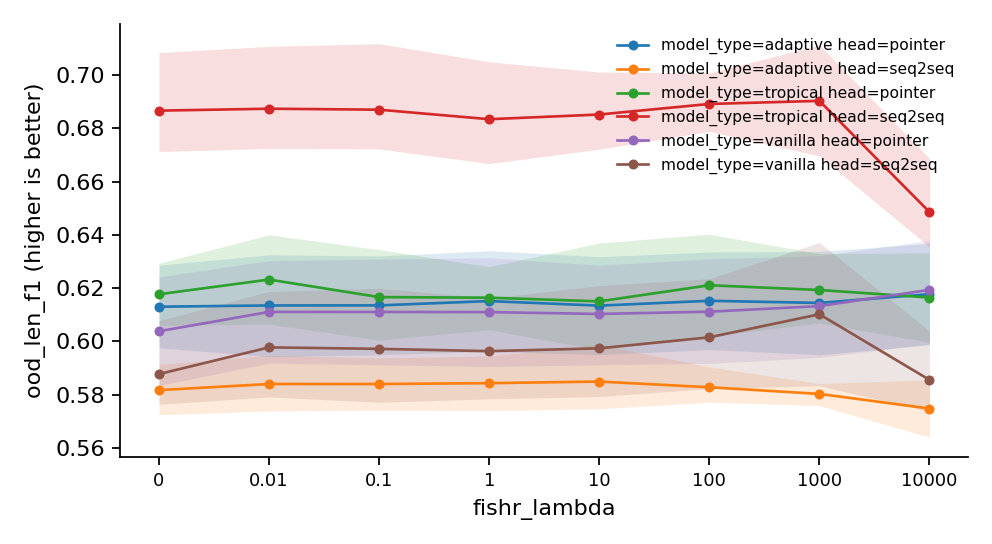
\includegraphics[width=\textwidth]{metric_ood_len_f1.png}
\caption{\texttt{ood\_len\_f1} against \texttt{fishr\_lambda}: the mean over seeds with a 95\% bootstrap CI, one line per combination of the other factors.}
\label{fig:ood_len_f1}
\end{figure}

{\small
\begin{longtable}{lllrlrrr}
\caption{\texttt{ood\_len\_f1} per cell: mean, 95\% bootstrap CI, SD, seeds, diverged runs.}\label{tab:summary-ood_len_f1}\\
\toprule
\texttt{model\_type} & \texttt{head} & \texttt{fishr\_lambda} & mean & 95\% CI & SD & $n$ & div.\\
\midrule
\endhead
adaptive & pointer & 0 & 0.6131 & [0.598, 0.629] & 0.0198 & 5 & 0\\
adaptive & pointer & 0.01 & 0.6135 & [0.594, 0.633] & 0.0252 & 5 & 0\\
adaptive & pointer & 0.1 & 0.6135 & [0.595, 0.632] & 0.0244 & 5 & 0\\
adaptive & pointer & 1 & 0.6152 & [0.596, 0.634] & 0.0241 & 5 & 0\\
adaptive & pointer & 10 & 0.6135 & [0.595, 0.632] & 0.0246 & 5 & 0\\
adaptive & pointer & 100 & 0.6153 & [0.597, 0.634] & 0.0234 & 5 & 0\\
adaptive & pointer & 1000 & 0.6145 & [0.595, 0.634] & 0.025 & 5 & 0\\
adaptive & pointer & 1e+04 & 0.6178 & [0.599, 0.637] & 0.024 & 5 & 0\\
adaptive & seq2seq & 0 & 0.5818 & [0.573, 0.591] & 0.0127 & 5 & 0\\
adaptive & seq2seq & 0.01 & 0.5841 & [0.574, 0.595] & 0.0143 & 5 & 0\\
adaptive & seq2seq & 0.1 & 0.584 & [0.574, 0.594] & 0.013 & 5 & 0\\
adaptive & seq2seq & 1 & 0.5844 & [0.574, 0.595] & 0.0138 & 5 & 0\\
adaptive & seq2seq & 10 & 0.585 & [0.575, 0.599] & 0.0152 & 5 & 0\\
adaptive & seq2seq & 100 & 0.5828 & [0.577, 0.59] & 0.00899 & 5 & 0\\
adaptive & seq2seq & 1000 & 0.5803 & [0.576, 0.584] & 0.00514 & 5 & 0\\
adaptive & seq2seq & 1e+04 & 0.5748 & [0.564, 0.586] & 0.014 & 5 & 0\\
tropical & pointer & 0 & 0.6177 & [0.606, 0.629] & 0.0158 & 5 & 0\\
tropical & pointer & 0.01 & 0.6232 & [0.607, 0.64] & 0.0219 & 5 & 0\\
tropical & pointer & 0.1 & 0.6167 & [0.601, 0.634] & 0.0215 & 5 & 0\\
tropical & pointer & 1 & 0.6164 & [0.604, 0.628] & 0.0155 & 5 & 0\\
tropical & pointer & 10 & 0.6151 & [0.597, 0.637] & 0.0262 & 5 & 0\\
tropical & pointer & 100 & 0.6211 & [0.602, 0.64] & 0.0253 & 5 & 0\\
tropical & pointer & 1000 & 0.6193 & [0.607, 0.633] & 0.016 & 5 & 0\\
tropical & pointer & 1e+04 & 0.6165 & [0.6, 0.633] & 0.0212 & 5 & 0\\
tropical & seq2seq & 0 & 0.6866 & [0.671, 0.708] & 0.025 & 5 & 0\\
tropical & seq2seq & 0.01 & 0.6873 & [0.672, 0.711] & 0.0256 & 5 & 0\\
tropical & seq2seq & 0.1 & 0.687 & [0.672, 0.712] & 0.0272 & 5 & 0\\
tropical & seq2seq & 1 & 0.6834 & [0.667, 0.705] & 0.0251 & 5 & 0\\
tropical & seq2seq & 10 & 0.6852 & [0.672, 0.701] & 0.0197 & 5 & 0\\
tropical & seq2seq & 100 & 0.6891 & [0.679, 0.701] & 0.0133 & 5 & 0\\
tropical & seq2seq & 1000 & 0.6903 & [0.67, 0.711] & 0.0264 & 5 & 0\\
tropical & seq2seq & 1e+04 & 0.6486 & [0.636, 0.669] & 0.0219 & 5 & 0\\
vanilla & pointer & 0 & 0.6038 & [0.583, 0.624] & 0.0273 & 5 & 0\\
vanilla & pointer & 0.01 & 0.6111 & [0.592, 0.63] & 0.0247 & 5 & 0\\
vanilla & pointer & 0.1 & 0.6111 & [0.591, 0.631] & 0.0255 & 5 & 0\\
vanilla & pointer & 1 & 0.611 & [0.591, 0.631] & 0.0259 & 5 & 0\\
vanilla & pointer & 10 & 0.6103 & [0.591, 0.629] & 0.0246 & 5 & 0\\
vanilla & pointer & 100 & 0.6112 & [0.592, 0.631] & 0.0252 & 5 & 0\\
vanilla & pointer & 1000 & 0.6133 & [0.594, 0.632] & 0.0243 & 5 & 0\\
vanilla & pointer & 1e+04 & 0.6194 & [0.599, 0.638] & 0.024 & 5 & 0\\
vanilla & seq2seq & 0 & 0.5878 & [0.576, 0.608] & 0.0221 & 5 & 0\\
vanilla & seq2seq & 0.01 & 0.5978 & [0.579, 0.619] & 0.0255 & 5 & 0\\
vanilla & seq2seq & 0.1 & 0.5972 & [0.577, 0.62] & 0.0273 & 5 & 0\\
vanilla & seq2seq & 1 & 0.5964 & [0.578, 0.616] & 0.0246 & 5 & 0\\
vanilla & seq2seq & 10 & 0.5974 & [0.579, 0.621] & 0.0264 & 5 & 0\\
vanilla & seq2seq & 100 & 0.6016 & [0.582, 0.624] & 0.0264 & 5 & 0\\
vanilla & seq2seq & 1000 & 0.6102 & [0.583, 0.637] & 0.0365 & 5 & 0\\
vanilla & seq2seq & 1e+04 & 0.5856 & [0.574, 0.604] & 0.0203 & 5 & 0\\
\bottomrule
\end{longtable}
}

{\small
\begin{longtable}{lllrrrl}
\caption{\texttt{ood\_len\_f1}: each level of \texttt{fishr\_lambda} against its control (0), within each combination of the other factors. parametric: Dunnett vs control.}\label{tab:control-ood_len_f1}\\
\toprule
\texttt{model\_type} & \texttt{head} & \texttt{fishr\_lambda} & difference & 95\% CI & $p$ & \\
\midrule
\endhead
adaptive & pointer & 0.01 & $4.704\times10^{-4}$ & [-0.0412, 0.0421] & 1.0000 & \\
adaptive & pointer & 0.1 & $4.955\times10^{-4}$ & [-0.0412, 0.0422] & 1.0000 & \\
adaptive & pointer & 1 & 0.002111 & [-0.0396, 0.0438] & 1.0000 & \\
adaptive & pointer & 10 & $4.038\times10^{-4}$ & [-0.0413, 0.0421] & 1.0000 & \\
adaptive & pointer & 100 & 0.002215 & [-0.0395, 0.0439] & 1.0000 & \\
adaptive & pointer & 1000 & 0.00142 & [-0.0402, 0.0431] & 1.0000 & \\
adaptive & pointer & 1e+04 & 0.004714 & [-0.037, 0.0464] & 0.9998 & \\
adaptive & seq2seq & 0.01 & 0.0023 & [-0.0196, 0.0242] & 0.9998 & \\
adaptive & seq2seq & 0.1 & 0.002296 & [-0.0196, 0.0242] & 0.9999 & \\
adaptive & seq2seq & 1 & 0.00262 & [-0.0193, 0.0245] & 0.9996 & \\
adaptive & seq2seq & 10 & 0.003213 & [-0.0187, 0.0251] & 0.9987 & \\
adaptive & seq2seq & 100 & 0.001079 & [-0.0208, 0.023] & 1.0000 & \\
adaptive & seq2seq & 1000 & -0.001416 & [-0.0233, 0.0205] & 1.0000 & \\
adaptive & seq2seq & 1e+04 & -0.006909 & [-0.0288, 0.015] & 0.9169 & \\
tropical & pointer & 0.01 & 0.005519 & [-0.0308, 0.0418] & 0.9984 & \\
tropical & pointer & 0.1 & -0.001068 & [-0.0374, 0.0353] & 1.0000 & \\
tropical & pointer & 1 & -0.001279 & [-0.0376, 0.035] & 1.0000 & \\
tropical & pointer & 10 & -0.002667 & [-0.039, 0.0337] & 1.0000 & \\
tropical & pointer & 100 & 0.003386 & [-0.0329, 0.0397] & 0.9999 & \\
tropical & pointer & 1000 & 0.001607 & [-0.0347, 0.0379] & 1.0000 & \\
tropical & pointer & 1e+04 & -0.001233 & [-0.0376, 0.0351] & 1.0000 & \\
tropical & seq2seq & 0.01 & $7.157\times10^{-4}$ & [-0.0402, 0.0416] & 1.0000 & \\
tropical & seq2seq & 0.1 & $3.535\times10^{-4}$ & [-0.0406, 0.0413] & 1.0000 & \\
tropical & seq2seq & 1 & -0.003218 & [-0.0442, 0.0377] & 1.0000 & \\
tropical & seq2seq & 10 & -0.001459 & [-0.0424, 0.0395] & 1.0000 & \\
tropical & seq2seq & 100 & 0.0025 & [-0.0384, 0.0434] & 1.0000 & \\
tropical & seq2seq & 1000 & 0.003661 & [-0.0373, 0.0446] & 0.9999 & \\
tropical & seq2seq & 1e+04 & -0.03806 & [-0.079, 0.00288] & 0.0770 & \\
vanilla & pointer & 0.01 & 0.007255 & [-0.0368, 0.0513] & 0.9974 & \\
vanilla & pointer & 0.1 & 0.007237 & [-0.0368, 0.0513] & 0.9974 & \\
vanilla & pointer & 1 & 0.007177 & [-0.0369, 0.0512] & 0.9975 & \\
vanilla & pointer & 10 & 0.006489 & [-0.0376, 0.0505] & 0.9987 & \\
vanilla & pointer & 100 & 0.007339 & [-0.0367, 0.0514] & 0.9972 & \\
vanilla & pointer & 1000 & 0.009424 & [-0.0346, 0.0535] & 0.9879 & \\
vanilla & pointer & 1e+04 & 0.01554 & [-0.0285, 0.0596] & 0.8684 & \\
vanilla & seq2seq & 0.01 & 0.01002 & [-0.0363, 0.0564] & 0.9872 & \\
vanilla & seq2seq & 0.1 & 0.009458 & [-0.0369, 0.0558] & 0.9907 & \\
vanilla & seq2seq & 1 & 0.008603 & [-0.0377, 0.055] & 0.9946 & \\
vanilla & seq2seq & 10 & 0.00966 & [-0.0367, 0.056] & 0.9896 & \\
vanilla & seq2seq & 100 & 0.01379 & [-0.0326, 0.0601] & 0.9358 & \\
vanilla & seq2seq & 1000 & 0.02244 & [-0.0239, 0.0688] & 0.6321 & \\
vanilla & seq2seq & 1e+04 & -0.002174 & [-0.0485, 0.0442] & 1.0000 & \\
\bottomrule
\end{longtable}
}

{\small
\begin{longtable}{llrrrrr}
\caption{\texttt{ood\_len\_f1} against log10 \texttt{fishr\_lambda}: parametric: OLS slope t-test, seed-bootstrap CI, with the Jonckheere--Terpstra ordered-trend $\tau$ and $p$.}\label{tab:trend-ood_len_f1}\\
\toprule
\texttt{model\_type} & \texttt{head} & estimate & 95\% CI & $p$ & JT $\tau$ & JT $p$\\
\midrule
\endhead
adaptive & pointer & $5.244\times10^{-4}$ & [$-3.53\times10^{-5}$, 0.00148] & 0.7842 & 0.0514 & 0.7075\\
adaptive & seq2seq & -0.001307 & [-0.00387, 0.00102] & 0.1962 & -0.0629 & 0.6395\\
tropical & pointer & $-3.658\times10^{-4}$ & [$-9.31\times10^{-4}$, $3.80\times10^{-4}$] & 0.8293 & -0.00571 & 0.9794\\
tropical & seq2seq & -0.003714 & [-0.00604, -0.00124] & 0.0808 & -0.143 & 0.2897\\
vanilla & pointer & 0.00105 & [$3.87\times10^{-4}$, 0.00189] & 0.5936 & 0.109 & 0.4181\\
vanilla & seq2seq & $-1.934\times10^{-4}$ & [$-5.01\times10^{-4}$, $1.13\times10^{-4}$] & 0.9302 & 0.0362 & 0.7964\\
\bottomrule
\end{longtable}
}

{\small
\begin{longtable}{lrrrl}
\caption{\texttt{ood\_len\_f1}: paired contrasts by seed, Holm-corrected across the cells. parametric: paired t-test by seed, Holm.}\label{tab:paired-ood_len_f1}\\
\toprule
contrast (within) & difference & 95\% CI & $p$ & \\
\midrule
\endhead
\stackcell{model\_type: tropical - vanilla\\\footnotesize head=pointer fishr\_lambda=0 } & 0.01387 & [-0.0164, 0.0441] & 1.0000 & \\
\stackcell{model\_type: tropical - vanilla\\\footnotesize head=pointer fishr\_lambda=0.01 } & 0.01214 & [-0.00917, 0.0334] & 1.0000 & \\
\stackcell{model\_type: tropical - vanilla\\\footnotesize head=pointer fishr\_lambda=0.1 } & 0.005568 & [-0.0228, 0.0339] & 1.0000 & \\
\stackcell{model\_type: tropical - vanilla\\\footnotesize head=pointer fishr\_lambda=1 } & 0.005418 & [-0.0188, 0.0297] & 1.0000 & \\
\stackcell{model\_type: tropical - vanilla\\\footnotesize head=pointer fishr\_lambda=10 } & 0.004717 & [-0.0232, 0.0327] & 1.0000 & \\
\stackcell{model\_type: tropical - vanilla\\\footnotesize head=pointer fishr\_lambda=100 } & 0.00992 & [-0.018, 0.0379] & 1.0000 & \\
\stackcell{model\_type: tropical - vanilla\\\footnotesize head=pointer fishr\_lambda=1000 } & 0.006056 & [-0.0139, 0.026] & 1.0000 & \\
\stackcell{model\_type: tropical - vanilla\\\footnotesize head=pointer fishr\_lambda=1e+04 } & -0.002901 & [-0.0255, 0.0197] & 1.0000 & \\
\stackcell{model\_type: tropical - vanilla\\\footnotesize head=seq2seq fishr\_lambda=0 } & 0.09885 & [0.0491, 0.149] & 0.0790 & \\
\stackcell{model\_type: tropical - vanilla\\\footnotesize head=seq2seq fishr\_lambda=0.01 } & 0.08955 & [0.0369, 0.142] & 0.1282 & \\
\stackcell{model\_type: tropical - vanilla\\\footnotesize head=seq2seq fishr\_lambda=0.1 } & 0.08975 & [0.0337, 0.146] & 0.1351 & \\
\stackcell{model\_type: tropical - vanilla\\\footnotesize head=seq2seq fishr\_lambda=1 } & 0.08703 & [0.0284, 0.146] & 0.1511 & \\
\stackcell{model\_type: tropical - vanilla\\\footnotesize head=seq2seq fishr\_lambda=10 } & 0.08773 & [0.0358, 0.14] & 0.1282 & \\
\stackcell{model\_type: tropical - vanilla\\\footnotesize head=seq2seq fishr\_lambda=100 } & 0.08756 & [0.0447, 0.13] & 0.0761 & \\
\stackcell{model\_type: tropical - vanilla\\\footnotesize head=seq2seq fishr\_lambda=1000 } & 0.08007 & [0.0134, 0.147] & 0.2611 & \\
\stackcell{model\_type: tropical - vanilla\\\footnotesize head=seq2seq fishr\_lambda=1e+04 } & 0.06297 & [0.0213, 0.105] & 0.1511 & \\
\stackcell{model\_type: adaptive - vanilla\\\footnotesize head=pointer fishr\_lambda=0 } & 0.009205 & [-0.00937, 0.0278] & 1.0000 & \\
\stackcell{model\_type: adaptive - vanilla\\\footnotesize head=pointer fishr\_lambda=0.01 } & 0.00242 & [$-3.62\times10^{-4}$, 0.0052] & 0.9509 & \\
\stackcell{model\_type: adaptive - vanilla\\\footnotesize head=pointer fishr\_lambda=0.1 } & 0.002463 & [$-7.97\times10^{-4}$, 0.00572] & 1.0000 & \\
\stackcell{model\_type: adaptive - vanilla\\\footnotesize head=pointer fishr\_lambda=1 } & 0.004139 & [0.00103, 0.00725] & 0.3133 & \\
\stackcell{model\_type: adaptive - vanilla\\\footnotesize head=pointer fishr\_lambda=10 } & 0.003119 & [$3.15\times10^{-4}$, 0.00592] & 0.5129 & \\
\stackcell{model\_type: adaptive - vanilla\\\footnotesize head=pointer fishr\_lambda=100 } & 0.004081 & [0.0017, 0.00646] & 0.1417 & \\
\stackcell{model\_type: adaptive - vanilla\\\footnotesize head=pointer fishr\_lambda=1000 } & 0.0012 & [-0.00371, 0.00611] & 1.0000 & \\
\stackcell{model\_type: adaptive - vanilla\\\footnotesize head=pointer fishr\_lambda=1e+04 } & -0.001622 & [-0.00446, 0.00121] & 1.0000 & \\
\stackcell{model\_type: adaptive - vanilla\\\footnotesize head=seq2seq fishr\_lambda=0 } & -0.006026 & [-0.0262, 0.0141] & 1.0000 & \\
\stackcell{model\_type: adaptive - vanilla\\\footnotesize head=seq2seq fishr\_lambda=0.01 } & -0.01374 & [-0.0423, 0.0148] & 1.0000 & \\
\stackcell{model\_type: adaptive - vanilla\\\footnotesize head=seq2seq fishr\_lambda=0.1 } & -0.01319 & [-0.0443, 0.0179] & 1.0000 & \\
\stackcell{model\_type: adaptive - vanilla\\\footnotesize head=seq2seq fishr\_lambda=1 } & -0.01201 & [-0.0379, 0.0139] & 1.0000 & \\
\stackcell{model\_type: adaptive - vanilla\\\footnotesize head=seq2seq fishr\_lambda=10 } & -0.01247 & [-0.035, 0.01] & 1.0000 & \\
\stackcell{model\_type: adaptive - vanilla\\\footnotesize head=seq2seq fishr\_lambda=100 } & -0.01874 & [-0.0449, 0.00742] & 1.0000 & \\
\stackcell{model\_type: adaptive - vanilla\\\footnotesize head=seq2seq fishr\_lambda=1000 } & -0.02989 & [-0.0762, 0.0165] & 1.0000 & \\
\stackcell{model\_type: adaptive - vanilla\\\footnotesize head=seq2seq fishr\_lambda=1e+04 } & -0.01076 & [-0.046, 0.0244] & 1.0000 & \\
\stackcell{head: pointer - seq2seq\\\footnotesize model\_type=adaptive fishr\_lambda=0 } & 0.0313 & [0.00424, 0.0584] & 0.4884 & \\
\stackcell{head: pointer - seq2seq\\\footnotesize model\_type=adaptive fishr\_lambda=0.01 } & 0.02947 & [-0.00502, 0.064] & 0.7317 & \\
\stackcell{head: pointer - seq2seq\\\footnotesize model\_type=adaptive fishr\_lambda=0.1 } & 0.0295 & [-0.00418, 0.0632] & 0.7317 & \\
\stackcell{head: pointer - seq2seq\\\footnotesize model\_type=adaptive fishr\_lambda=1 } & 0.03079 & [-0.00336, 0.0649] & 0.7317 & \\
\stackcell{head: pointer - seq2seq\\\footnotesize model\_type=adaptive fishr\_lambda=10 } & 0.02849 & [-0.00317, 0.0602] & 0.7317 & \\
\stackcell{head: pointer - seq2seq\\\footnotesize model\_type=adaptive fishr\_lambda=100 } & 0.03244 & [0.005, 0.0599] & 0.4869 & \\
\stackcell{head: pointer - seq2seq\\\footnotesize model\_type=adaptive fishr\_lambda=1000 } & 0.03414 & [-0.00227, 0.0705] & 0.7181 & \\
\stackcell{head: pointer - seq2seq\\\footnotesize model\_type=adaptive fishr\_lambda=1e+04 } & 0.04293 & [0.00424, 0.0816] & 0.5167 & \\
\stackcell{head: pointer - seq2seq\\\footnotesize model\_type=tropical fishr\_lambda=0 } & -0.06891 & [-0.0986, -0.0392] & 0.0654 & \\
\stackcell{head: pointer - seq2seq\\\footnotesize model\_type=tropical fishr\_lambda=0.01 } & -0.0641 & [-0.0981, -0.0301] & 0.1211 & \\
\stackcell{head: pointer - seq2seq\\\footnotesize model\_type=tropical fishr\_lambda=0.1 } & -0.07033 & [-0.104, -0.0366] & 0.0888 & \\
\stackcell{head: pointer - seq2seq\\\footnotesize model\_type=tropical fishr\_lambda=1 } & -0.06697 & [-0.0971, -0.0369] & 0.0733 & \\
\stackcell{head: pointer - seq2seq\\\footnotesize model\_type=tropical fishr\_lambda=10 } & -0.07012 & [-0.0974, -0.0429] & 0.0487 & *\\
\stackcell{head: pointer - seq2seq\\\footnotesize model\_type=tropical fishr\_lambda=100 } & -0.06802 & [-0.0952, -0.0409] & 0.0517 & \\
\stackcell{head: pointer - seq2seq\\\footnotesize model\_type=tropical fishr\_lambda=1000 } & -0.07096 & [-0.118, -0.0237] & 0.2536 & \\
\stackcell{head: pointer - seq2seq\\\footnotesize model\_type=tropical fishr\_lambda=1e+04 } & -0.03208 & [-0.0621, -0.00204] & 0.5375 & \\
\stackcell{head: pointer - seq2seq\\\footnotesize model\_type=vanilla fishr\_lambda=0 } & 0.01607 & [-0.00908, 0.0412] & 1.0000 & \\
\stackcell{head: pointer - seq2seq\\\footnotesize model\_type=vanilla fishr\_lambda=0.01 } & 0.01331 & [-0.0219, 0.0485] & 1.0000 & \\
\stackcell{head: pointer - seq2seq\\\footnotesize model\_type=vanilla fishr\_lambda=0.1 } & 0.01385 & [-0.023, 0.0507] & 1.0000 & \\
\stackcell{head: pointer - seq2seq\\\footnotesize model\_type=vanilla fishr\_lambda=1 } & 0.01465 & [-0.0225, 0.0518] & 1.0000 & \\
\stackcell{head: pointer - seq2seq\\\footnotesize model\_type=vanilla fishr\_lambda=10 } & 0.0129 & [-0.0211, 0.0469] & 1.0000 & \\
\stackcell{head: pointer - seq2seq\\\footnotesize model\_type=vanilla fishr\_lambda=100 } & 0.009619 & [-0.0298, 0.0491] & 1.0000 & \\
\stackcell{head: pointer - seq2seq\\\footnotesize model\_type=vanilla fishr\_lambda=1000 } & 0.003052 & [-0.0492, 0.0553] & 1.0000 & \\
\stackcell{head: pointer - seq2seq\\\footnotesize model\_type=vanilla fishr\_lambda=1e+04 } & 0.03379 & [0.00843, 0.0591] & 0.3545 & \\
\bottomrule
\end{longtable}
}

\clearpage
\appendix
\section{Other metrics}
\subsection{\texttt{ood\_len\_exact}}
\begin{figure}[tbp]
\centering
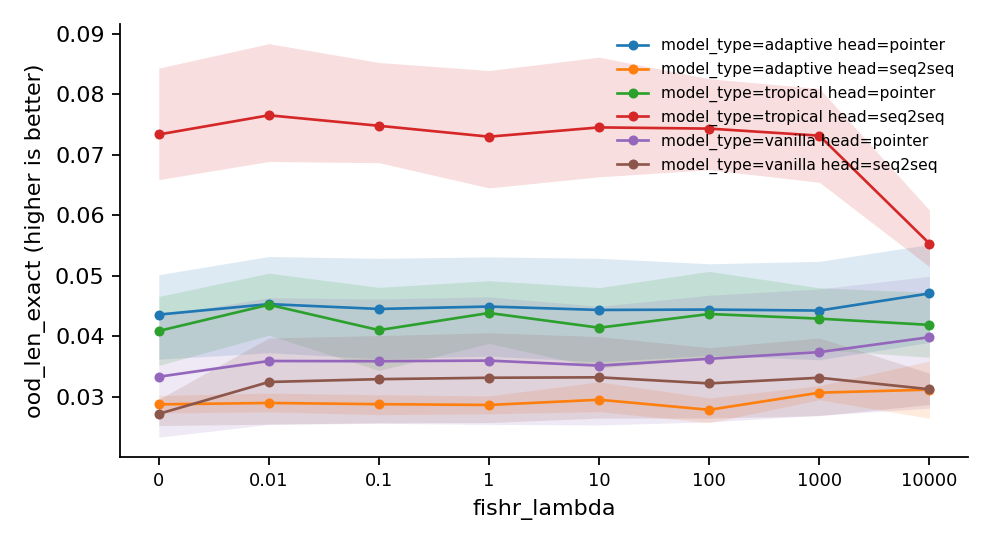
\includegraphics[width=\textwidth]{metric_ood_len_exact.png}
\caption{\texttt{ood\_len\_exact} against \texttt{fishr\_lambda}: the mean over seeds with a 95\% bootstrap CI, one line per combination of the other factors.}
\label{fig:ood_len_exact}
\end{figure}

{\small
\begin{longtable}{lllrlrrr}
\caption{\texttt{ood\_len\_exact} per cell: mean, 95\% bootstrap CI, SD, seeds, diverged runs.}\label{tab:summary-ood_len_exact}\\
\toprule
\texttt{model\_type} & \texttt{head} & \texttt{fishr\_lambda} & mean & 95\% CI & SD & $n$ & div.\\
\midrule
\endhead
adaptive & pointer & 0 & 0.0436 & [0.0362, 0.0502] & 0.00887 & 5 & 0\\
adaptive & pointer & 0.01 & 0.04533 & [0.0373, 0.0532] & 0.0105 & 5 & 0\\
adaptive & pointer & 0.1 & 0.04453 & [0.0363, 0.0529] & 0.0106 & 5 & 0\\
adaptive & pointer & 1 & 0.04493 & [0.0367, 0.0531] & 0.0107 & 5 & 0\\
adaptive & pointer & 10 & 0.04437 & [0.0358, 0.0529] & 0.0109 & 5 & 0\\
adaptive & pointer & 100 & 0.04443 & [0.0369, 0.052] & 0.00975 & 5 & 0\\
adaptive & pointer & 1000 & 0.04427 & [0.0361, 0.0524] & 0.0104 & 5 & 0\\
adaptive & pointer & 1e+04 & 0.0471 & [0.039, 0.0552] & 0.0103 & 5 & 0\\
adaptive & seq2seq & 0 & 0.02877 & [0.0273, 0.0302] & 0.00187 & 5 & 0\\
adaptive & seq2seq & 0.01 & 0.029 & [0.0275, 0.0306] & 0.00197 & 5 & 0\\
adaptive & seq2seq & 0.1 & 0.0288 & [0.0271, 0.0304] & 0.00213 & 5 & 0\\
adaptive & seq2seq & 1 & 0.02867 & [0.0272, 0.0302] & 0.00193 & 5 & 0\\
adaptive & seq2seq & 10 & 0.02953 & [0.0276, 0.0325] & 0.00324 & 5 & 0\\
adaptive & seq2seq & 100 & 0.02787 & [0.0257, 0.0298] & 0.00259 & 5 & 0\\
adaptive & seq2seq & 1000 & 0.0307 & [0.0295, 0.0319] & 0.0015 & 5 & 0\\
adaptive & seq2seq & 1e+04 & 0.0312 & [0.0265, 0.0359] & 0.00615 & 5 & 0\\
tropical & pointer & 0 & 0.0409 & [0.0352, 0.0466] & 0.00734 & 5 & 0\\
tropical & pointer & 0.01 & 0.04523 & [0.0402, 0.0504] & 0.00673 & 5 & 0\\
tropical & pointer & 0.1 & 0.04103 & [0.0344, 0.0481] & 0.00885 & 5 & 0\\
tropical & pointer & 1 & 0.04387 & [0.0388, 0.0492] & 0.00661 & 5 & 0\\
tropical & pointer & 10 & 0.04143 & [0.0348, 0.0481] & 0.00833 & 5 & 0\\
tropical & pointer & 100 & 0.0437 & [0.0363, 0.0507] & 0.00918 & 5 & 0\\
tropical & pointer & 1000 & 0.04293 & [0.0378, 0.048] & 0.00669 & 5 & 0\\
tropical & pointer & 1e+04 & 0.0419 & [0.0365, 0.0473] & 0.00729 & 5 & 0\\
tropical & seq2seq & 0 & 0.07337 & [0.0659, 0.0843] & 0.0124 & 5 & 0\\
tropical & seq2seq & 0.01 & 0.07653 & [0.0689, 0.0884] & 0.0135 & 5 & 0\\
tropical & seq2seq & 0.1 & 0.0748 & [0.0687, 0.0853] & 0.0118 & 5 & 0\\
tropical & seq2seq & 1 & 0.073 & [0.0645, 0.0839] & 0.0131 & 5 & 0\\
tropical & seq2seq & 10 & 0.07453 & [0.0664, 0.0861] & 0.0129 & 5 & 0\\
tropical & seq2seq & 100 & 0.07433 & [0.0675, 0.0826] & 0.00937 & 5 & 0\\
tropical & seq2seq & 1000 & 0.07317 & [0.0655, 0.081] & 0.0103 & 5 & 0\\
tropical & seq2seq & 1e+04 & 0.05533 & [0.0515, 0.0609] & 0.00623 & 5 & 0\\
vanilla & pointer & 0 & 0.03333 & [0.0233, 0.0434] & 0.0135 & 5 & 0\\
vanilla & pointer & 0.01 & 0.03593 & [0.0255, 0.0464] & 0.0135 & 5 & 0\\
vanilla & pointer & 0.1 & 0.0359 & [0.0256, 0.0462] & 0.0134 & 5 & 0\\
vanilla & pointer & 1 & 0.036 & [0.0255, 0.0465] & 0.0137 & 5 & 0\\
vanilla & pointer & 10 & 0.03517 & [0.0254, 0.045] & 0.0131 & 5 & 0\\
vanilla & pointer & 100 & 0.0363 & [0.0259, 0.0468] & 0.0134 & 5 & 0\\
vanilla & pointer & 1000 & 0.0374 & [0.027, 0.0478] & 0.0136 & 5 & 0\\
vanilla & pointer & 1e+04 & 0.03987 & [0.0281, 0.0499] & 0.0138 & 5 & 0\\
vanilla & seq2seq & 0 & 0.0272 & [0.0253, 0.0296] & 0.00273 & 5 & 0\\
vanilla & seq2seq & 0.01 & 0.03247 & [0.0255, 0.0397] & 0.00919 & 5 & 0\\
vanilla & seq2seq & 0.1 & 0.03293 & [0.0257, 0.0401] & 0.00946 & 5 & 0\\
vanilla & seq2seq & 1 & 0.03317 & [0.0258, 0.0406] & 0.00968 & 5 & 0\\
vanilla & seq2seq & 10 & 0.03323 & [0.0265, 0.04] & 0.0087 & 5 & 0\\
vanilla & seq2seq & 100 & 0.03223 & [0.0265, 0.0381] & 0.00749 & 5 & 0\\
vanilla & seq2seq & 1000 & 0.03317 & [0.0269, 0.0397] & 0.0083 & 5 & 0\\
vanilla & seq2seq & 1e+04 & 0.03127 & [0.0287, 0.0339] & 0.00367 & 5 & 0\\
\bottomrule
\end{longtable}
}

{\small
\begin{longtable}{lllrrrl}
\caption{\texttt{ood\_len\_exact}: each level of \texttt{fishr\_lambda} against its control (0), within each combination of the other factors. parametric: Dunnett vs control.}\label{tab:control-ood_len_exact}\\
\toprule
\texttt{model\_type} & \texttt{head} & \texttt{fishr\_lambda} & difference & 95\% CI & $p$ & \\
\midrule
\endhead
adaptive & pointer & 0.01 & 0.001733 & [-0.0162, 0.0197] & 0.9999 & \\
adaptive & pointer & 0.1 & $9.333\times10^{-4}$ & [-0.017, 0.0189] & 1.0000 & \\
adaptive & pointer & 1 & 0.001333 & [-0.0166, 0.0193] & 1.0000 & \\
adaptive & pointer & 10 & $7.667\times10^{-4}$ & [-0.0172, 0.0187] & 1.0000 & \\
adaptive & pointer & 100 & $8.333\times10^{-4}$ & [-0.0171, 0.0188] & 1.0000 & \\
adaptive & pointer & 1000 & $6.667\times10^{-4}$ & [-0.0173, 0.0186] & 1.0000 & \\
adaptive & pointer & 1e+04 & 0.0035 & [-0.0144, 0.0214] & 0.9928 & \\
adaptive & seq2seq & 0.01 & $2.333\times10^{-4}$ & [-0.00504, 0.00551] & 1.0000 & \\
adaptive & seq2seq & 0.1 & $3.333\times10^{-5}$ & [-0.00524, 0.00531] & 1.0000 & \\
adaptive & seq2seq & 1 & $-1.000\times10^{-4}$ & [-0.00537, 0.00517] & 1.0000 & \\
adaptive & seq2seq & 10 & $7.667\times10^{-4}$ & [-0.00451, 0.00604] & 0.9988 & \\
adaptive & seq2seq & 100 & $-9.000\times10^{-4}$ & [-0.00617, 0.00437] & 0.9967 & \\
adaptive & seq2seq & 1000 & 0.001933 & [-0.00334, 0.00721] & 0.8474 & \\
adaptive & seq2seq & 1e+04 & 0.002433 & [-0.00284, 0.00771] & 0.6768 & \\
tropical & pointer & 0.01 & 0.004333 & [-0.00909, 0.0178] & 0.9082 & \\
tropical & pointer & 0.1 & $1.333\times10^{-4}$ & [-0.0133, 0.0136] & 1.0000 & \\
tropical & pointer & 1 & 0.002967 & [-0.0105, 0.0164] & 0.9856 & \\
tropical & pointer & 10 & $5.333\times10^{-4}$ & [-0.0129, 0.014] & 1.0000 & \\
tropical & pointer & 100 & 0.0028 & [-0.0106, 0.0162] & 0.9895 & \\
tropical & pointer & 1000 & 0.002033 & [-0.0114, 0.0155] & 0.9984 & \\
tropical & pointer & 1e+04 & 0.001 & [-0.0124, 0.0144] & 1.0000 & \\
tropical & seq2seq & 0.01 & 0.003167 & [-0.0168, 0.0231] & 0.9979 & \\
tropical & seq2seq & 0.1 & 0.001433 & [-0.0185, 0.0214] & 1.0000 & \\
tropical & seq2seq & 1 & $-3.667\times10^{-4}$ & [-0.0203, 0.0196] & 1.0000 & \\
tropical & seq2seq & 10 & 0.001167 & [-0.0188, 0.0211] & 1.0000 & \\
tropical & seq2seq & 100 & $9.667\times10^{-4}$ & [-0.019, 0.0209] & 1.0000 & \\
tropical & seq2seq & 1000 & $-2.000\times10^{-4}$ & [-0.0202, 0.0198] & 1.0000 & \\
tropical & seq2seq & 1e+04 & -0.01803 & [-0.038, 0.00195] & 0.0904 & \\
vanilla & pointer & 0.01 & 0.0026 & [-0.021, 0.0262] & 0.9998 & \\
vanilla & pointer & 0.1 & 0.002567 & [-0.021, 0.0262] & 0.9998 & \\
vanilla & pointer & 1 & 0.002667 & [-0.0209, 0.0263] & 0.9998 & \\
vanilla & pointer & 10 & 0.001833 & [-0.0218, 0.0254] & 1.0000 & \\
vanilla & pointer & 100 & 0.002967 & [-0.0206, 0.0266] & 0.9995 & \\
vanilla & pointer & 1000 & 0.004067 & [-0.0195, 0.0277] & 0.9965 & \\
vanilla & pointer & 1e+04 & 0.006533 & [-0.0171, 0.0301] & 0.9540 & \\
vanilla & seq2seq & 0.01 & 0.005267 & [-0.00839, 0.0189] & 0.8167 & \\
vanilla & seq2seq & 0.1 & 0.005733 & [-0.00793, 0.0194] & 0.7565 & \\
vanilla & seq2seq & 1 & 0.005967 & [-0.00769, 0.0196] & 0.7243 & \\
vanilla & seq2seq & 10 & 0.006033 & [-0.00763, 0.0197] & 0.7150 & \\
vanilla & seq2seq & 100 & 0.005033 & [-0.00863, 0.0187] & 0.8445 & \\
vanilla & seq2seq & 1000 & 0.005967 & [-0.00769, 0.0196] & 0.7243 & \\
vanilla & seq2seq & 1e+04 & 0.004067 & [-0.00959, 0.0177] & 0.9357 & \\
\bottomrule
\end{longtable}
}

{\small
\begin{longtable}{llrrrrr}
\caption{\texttt{ood\_len\_exact} against log10 \texttt{fishr\_lambda}: parametric: OLS slope t-test, seed-bootstrap CI, with the Jonckheere--Terpstra ordered-trend $\tau$ and $p$.}\label{tab:trend-ood_len_exact}\\
\toprule
\texttt{model\_type} & \texttt{head} & estimate & 95\% CI & $p$ & JT $\tau$ & JT $p$\\
\midrule
\endhead
adaptive & pointer & $1.524\times10^{-4}$ & [$-2.26\times10^{-4}$, $5.17\times10^{-4}$] & 0.8531 & -0.0133 & 0.9224\\
adaptive & seq2seq & $3.429\times10^{-4}$ & [$-2.38\times10^{-4}$, $8.18\times10^{-4}$] & 0.1898 & 0.0705 & 0.6169\\
tropical & pointer & $-2.274\times10^{-4}$ & [$-5.62\times10^{-4}$, $1.67\times10^{-4}$] & 0.7131 & -0.0552 & 0.6689\\
tropical & seq2seq & -0.00234 & [-0.0036, -0.0013] & 0.0223 & -0.278 & 0.0410\\
vanilla & pointer & $5.393\times10^{-4}$ & [$2.43\times10^{-4}$, $9.45\times10^{-4}$] & 0.6126 & 0.0971 & 0.4719\\
vanilla & seq2seq & $-1.452\times10^{-4}$ & [$-8.81\times10^{-4}$, $4.36\times10^{-4}$] & 0.8240 & 0.061 & 0.6559\\
\bottomrule
\end{longtable}
}

{\small
\begin{longtable}{lrrrl}
\caption{\texttt{ood\_len\_exact}: paired contrasts by seed, Holm-corrected across the cells. parametric: paired t-test by seed, Holm.}\label{tab:paired-ood_len_exact}\\
\toprule
contrast (within) & difference & 95\% CI & $p$ & \\
\midrule
\endhead
\stackcell{model\_type: tropical - vanilla\\\footnotesize head=pointer fishr\_lambda=0 } & 0.007567 & [-0.0133, 0.0284] & 1.0000 & \\
\stackcell{model\_type: tropical - vanilla\\\footnotesize head=pointer fishr\_lambda=0.01 } & 0.0093 & [-0.00944, 0.028] & 1.0000 & \\
\stackcell{model\_type: tropical - vanilla\\\footnotesize head=pointer fishr\_lambda=0.1 } & 0.005133 & [-0.0171, 0.0273] & 1.0000 & \\
\stackcell{model\_type: tropical - vanilla\\\footnotesize head=pointer fishr\_lambda=1 } & 0.007867 & [-0.0139, 0.0296] & 1.0000 & \\
\stackcell{model\_type: tropical - vanilla\\\footnotesize head=pointer fishr\_lambda=10 } & 0.006267 & [-0.0149, 0.0275] & 1.0000 & \\
\stackcell{model\_type: tropical - vanilla\\\footnotesize head=pointer fishr\_lambda=100 } & 0.0074 & [-0.0137, 0.0285] & 1.0000 & \\
\stackcell{model\_type: tropical - vanilla\\\footnotesize head=pointer fishr\_lambda=1000 } & 0.005533 & [-0.0139, 0.0249] & 1.0000 & \\
\stackcell{model\_type: tropical - vanilla\\\footnotesize head=pointer fishr\_lambda=1e+04 } & 0.002033 & [-0.0204, 0.0245] & 1.0000 & \\
\stackcell{model\_type: tropical - vanilla\\\footnotesize head=seq2seq fishr\_lambda=0 } & 0.04617 & [0.0291, 0.0632] & 0.0268 & *\\
\stackcell{model\_type: tropical - vanilla\\\footnotesize head=seq2seq fishr\_lambda=0.01 } & 0.04407 & [0.0191, 0.069] & 0.0886 & \\
\stackcell{model\_type: tropical - vanilla\\\footnotesize head=seq2seq fishr\_lambda=0.1 } & 0.04187 & [0.0196, 0.0642] & 0.0840 & \\
\stackcell{model\_type: tropical - vanilla\\\footnotesize head=seq2seq fishr\_lambda=1 } & 0.03983 & [0.013, 0.0667] & 0.1318 & \\
\stackcell{model\_type: tropical - vanilla\\\footnotesize head=seq2seq fishr\_lambda=10 } & 0.0413 & [0.0171, 0.0655] & 0.0900 & \\
\stackcell{model\_type: tropical - vanilla\\\footnotesize head=seq2seq fishr\_lambda=100 } & 0.0421 & [0.0232, 0.061] & 0.0486 & *\\
\stackcell{model\_type: tropical - vanilla\\\footnotesize head=seq2seq fishr\_lambda=1000 } & 0.04 & [0.0186, 0.0614] & 0.0840 & \\
\stackcell{model\_type: tropical - vanilla\\\footnotesize head=seq2seq fishr\_lambda=1e+04 } & 0.02407 & [0.014, 0.0341] & 0.0400 & *\\
\stackcell{model\_type: adaptive - vanilla\\\footnotesize head=pointer fishr\_lambda=0 } & 0.01027 & [-0.00237, 0.0229] & 0.7845 & \\
\stackcell{model\_type: adaptive - vanilla\\\footnotesize head=pointer fishr\_lambda=0.01 } & 0.0094 & [0.0045, 0.0143] & 0.0956 & \\
\stackcell{model\_type: adaptive - vanilla\\\footnotesize head=pointer fishr\_lambda=0.1 } & 0.008633 & [0.00327, 0.014] & 0.1660 & \\
\stackcell{model\_type: adaptive - vanilla\\\footnotesize head=pointer fishr\_lambda=1 } & 0.008933 & [0.00245, 0.0154] & 0.2246 & \\
\stackcell{model\_type: adaptive - vanilla\\\footnotesize head=pointer fishr\_lambda=10 } & 0.0092 & [0.00286, 0.0155] & 0.2048 & \\
\stackcell{model\_type: adaptive - vanilla\\\footnotesize head=pointer fishr\_lambda=100 } & 0.008133 & [0.00279, 0.0135] & 0.1882 & \\
\stackcell{model\_type: adaptive - vanilla\\\footnotesize head=pointer fishr\_lambda=1000 } & 0.006867 & [$6.30\times10^{-4}$, 0.0131] & 0.3777 & \\
\stackcell{model\_type: adaptive - vanilla\\\footnotesize head=pointer fishr\_lambda=1e+04 } & 0.007233 & [0.00112, 0.0133] & 0.3331 & \\
\stackcell{model\_type: adaptive - vanilla\\\footnotesize head=seq2seq fishr\_lambda=0 } & 0.001567 & [$-8.49\times10^{-4}$, 0.00398] & 1.0000 & \\
\stackcell{model\_type: adaptive - vanilla\\\footnotesize head=seq2seq fishr\_lambda=0.01 } & -0.003467 & [-0.0143, 0.00734] & 1.0000 & \\
\stackcell{model\_type: adaptive - vanilla\\\footnotesize head=seq2seq fishr\_lambda=0.1 } & -0.004133 & [-0.0155, 0.00725] & 1.0000 & \\
\stackcell{model\_type: adaptive - vanilla\\\footnotesize head=seq2seq fishr\_lambda=1 } & -0.0045 & [-0.016, 0.007] & 1.0000 & \\
\stackcell{model\_type: adaptive - vanilla\\\footnotesize head=seq2seq fishr\_lambda=10 } & -0.0037 & [-0.0137, 0.00631] & 1.0000 & \\
\stackcell{model\_type: adaptive - vanilla\\\footnotesize head=seq2seq fishr\_lambda=100 } & -0.004367 & [-0.0135, 0.0048] & 1.0000 & \\
\stackcell{model\_type: adaptive - vanilla\\\footnotesize head=seq2seq fishr\_lambda=1000 } & -0.002467 & [-0.0136, 0.0087] & 1.0000 & \\
\stackcell{model\_type: adaptive - vanilla\\\footnotesize head=seq2seq fishr\_lambda=1e+04 } & $-6.667\times10^{-5}$ & [-0.011, 0.0108] & 1.0000 & \\
\stackcell{head: pointer - seq2seq\\\footnotesize model\_type=adaptive fishr\_lambda=0 } & 0.01483 & [0.00448, 0.0252] & 0.2555 & \\
\stackcell{head: pointer - seq2seq\\\footnotesize model\_type=adaptive fishr\_lambda=0.01 } & 0.01633 & [0.00503, 0.0276] & 0.2555 & \\
\stackcell{head: pointer - seq2seq\\\footnotesize model\_type=adaptive fishr\_lambda=0.1 } & 0.01573 & [0.00425, 0.0272] & 0.2664 & \\
\stackcell{head: pointer - seq2seq\\\footnotesize model\_type=adaptive fishr\_lambda=1 } & 0.01627 & [0.00413, 0.0284] & 0.2664 & \\
\stackcell{head: pointer - seq2seq\\\footnotesize model\_type=adaptive fishr\_lambda=10 } & 0.01483 & [0.00349, 0.0262] & 0.2664 & \\
\stackcell{head: pointer - seq2seq\\\footnotesize model\_type=adaptive fishr\_lambda=100 } & 0.01657 & [0.00673, 0.0264] & 0.1992 & \\
\stackcell{head: pointer - seq2seq\\\footnotesize model\_type=adaptive fishr\_lambda=1000 } & 0.01357 & [$-8.19\times10^{-4}$, 0.028] & 0.5810 & \\
\stackcell{head: pointer - seq2seq\\\footnotesize model\_type=adaptive fishr\_lambda=1e+04 } & 0.0159 & [$8.74\times10^{-4}$, 0.0309] & 0.4673 & \\
\stackcell{head: pointer - seq2seq\\\footnotesize model\_type=tropical fishr\_lambda=0 } & -0.03247 & [-0.0531, -0.0118] & 0.2277 & \\
\stackcell{head: pointer - seq2seq\\\footnotesize model\_type=tropical fishr\_lambda=0.01 } & -0.0313 & [-0.0515, -0.0111] & 0.2277 & \\
\stackcell{head: pointer - seq2seq\\\footnotesize model\_type=tropical fishr\_lambda=0.1 } & -0.03377 & [-0.0544, -0.0131] & 0.2093 & \\
\stackcell{head: pointer - seq2seq\\\footnotesize model\_type=tropical fishr\_lambda=1 } & -0.02913 & [-0.0479, -0.0103] & 0.2277 & \\
\stackcell{head: pointer - seq2seq\\\footnotesize model\_type=tropical fishr\_lambda=10 } & -0.0331 & [-0.0522, -0.014] & 0.1904 & \\
\stackcell{head: pointer - seq2seq\\\footnotesize model\_type=tropical fishr\_lambda=100 } & -0.03063 & [-0.0471, -0.0142] & 0.1607 & \\
\stackcell{head: pointer - seq2seq\\\footnotesize model\_type=tropical fishr\_lambda=1000 } & -0.03023 & [-0.0469, -0.0136] & 0.1682 & \\
\stackcell{head: pointer - seq2seq\\\footnotesize model\_type=tropical fishr\_lambda=1e+04 } & -0.01343 & [-0.0276, $7.40\times10^{-4}$] & 0.5810 & \\
\stackcell{head: pointer - seq2seq\\\footnotesize model\_type=vanilla fishr\_lambda=0 } & 0.006133 & [-0.00832, 0.0206] & 1.0000 & \\
\stackcell{head: pointer - seq2seq\\\footnotesize model\_type=vanilla fishr\_lambda=0.01 } & 0.003467 & [-0.0159, 0.0228] & 1.0000 & \\
\stackcell{head: pointer - seq2seq\\\footnotesize model\_type=vanilla fishr\_lambda=0.1 } & 0.002967 & [-0.0158, 0.0217] & 1.0000 & \\
\stackcell{head: pointer - seq2seq\\\footnotesize model\_type=vanilla fishr\_lambda=1 } & 0.002833 & [-0.0165, 0.0222] & 1.0000 & \\
\stackcell{head: pointer - seq2seq\\\footnotesize model\_type=vanilla fishr\_lambda=10 } & 0.001933 & [-0.0155, 0.0193] & 1.0000 & \\
\stackcell{head: pointer - seq2seq\\\footnotesize model\_type=vanilla fishr\_lambda=100 } & 0.004067 & [-0.0148, 0.023] & 1.0000 & \\
\stackcell{head: pointer - seq2seq\\\footnotesize model\_type=vanilla fishr\_lambda=1000 } & 0.004233 & [-0.015, 0.0234] & 1.0000 & \\
\stackcell{head: pointer - seq2seq\\\footnotesize model\_type=vanilla fishr\_lambda=1e+04 } & 0.0086 & [-0.00717, 0.0244] & 1.0000 & \\
\bottomrule
\end{longtable}
}

\subsection{\texttt{ood\_val\_f1}}
\begin{figure}[tbp]
\centering
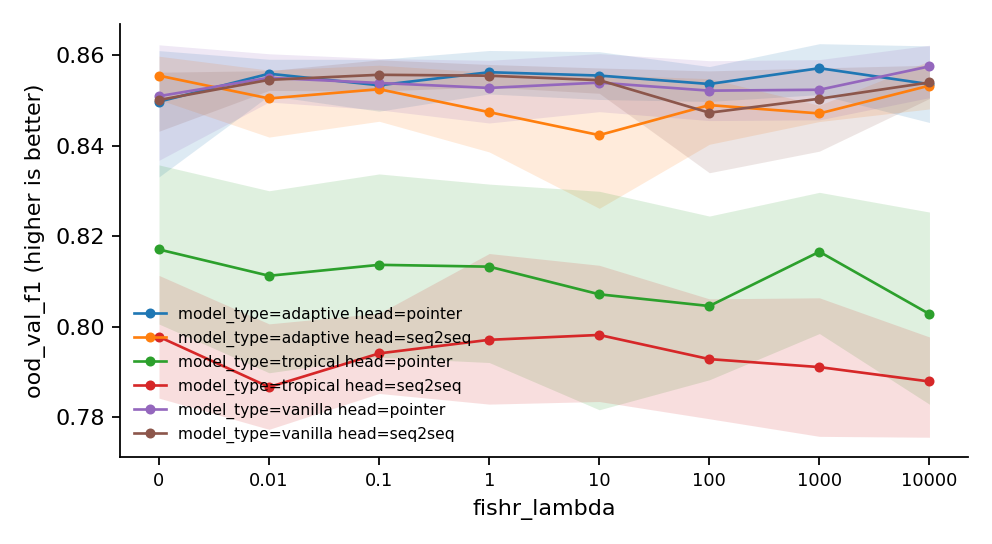
\includegraphics[width=\textwidth]{metric_ood_val_f1.png}
\caption{\texttt{ood\_val\_f1} against \texttt{fishr\_lambda}: the mean over seeds with a 95\% bootstrap CI, one line per combination of the other factors.}
\label{fig:ood_val_f1}
\end{figure}

{\small
\begin{longtable}{lllrlrrr}
\caption{\texttt{ood\_val\_f1} per cell: mean, 95\% bootstrap CI, SD, seeds, diverged runs.}\label{tab:summary-ood_val_f1}\\
\toprule
\texttt{model\_type} & \texttt{head} & \texttt{fishr\_lambda} & mean & 95\% CI & SD & $n$ & div.\\
\midrule
\endhead
adaptive & pointer & 0 & 0.8498 & [0.833, 0.861] & 0.0172 & 5 & 0\\
adaptive & pointer & 0.01 & 0.8559 & [0.851, 0.859] & 0.00539 & 5 & 0\\
adaptive & pointer & 0.1 & 0.8534 & [0.848, 0.859] & 0.00739 & 5 & 0\\
adaptive & pointer & 1 & 0.8563 & [0.851, 0.861] & 0.0062 & 5 & 0\\
adaptive & pointer & 10 & 0.8555 & [0.85, 0.861] & 0.00677 & 5 & 0\\
adaptive & pointer & 100 & 0.8537 & [0.85, 0.858] & 0.00514 & 5 & 0\\
adaptive & pointer & 1000 & 0.8572 & [0.851, 0.863] & 0.00768 & 5 & 0\\
adaptive & pointer & 1e+04 & 0.8536 & [0.845, 0.862] & 0.0115 & 5 & 0\\
adaptive & seq2seq & 0 & 0.8555 & [0.85, 0.86] & 0.00636 & 5 & 0\\
adaptive & seq2seq & 0.01 & 0.8505 & [0.842, 0.857] & 0.0101 & 5 & 0\\
adaptive & seq2seq & 0.1 & 0.8525 & [0.845, 0.858] & 0.00829 & 5 & 0\\
adaptive & seq2seq & 1 & 0.8474 & [0.839, 0.856] & 0.0118 & 5 & 0\\
adaptive & seq2seq & 10 & 0.8424 & [0.826, 0.856] & 0.0202 & 5 & 0\\
adaptive & seq2seq & 100 & 0.849 & [0.84, 0.855] & 0.00972 & 5 & 0\\
adaptive & seq2seq & 1000 & 0.8472 & [0.845, 0.849] & 0.0024 & 5 & 0\\
adaptive & seq2seq & 1e+04 & 0.8533 & [0.848, 0.859] & 0.00696 & 5 & 0\\
tropical & pointer & 0 & 0.8171 & [0.801, 0.836] & 0.0222 & 5 & 0\\
tropical & pointer & 0.01 & 0.8112 & [0.79, 0.83] & 0.0261 & 5 & 0\\
tropical & pointer & 0.1 & 0.8137 & [0.793, 0.834] & 0.026 & 5 & 0\\
tropical & pointer & 1 & 0.8133 & [0.792, 0.832] & 0.0254 & 5 & 0\\
tropical & pointer & 10 & 0.8071 & [0.782, 0.83] & 0.0307 & 5 & 0\\
tropical & pointer & 100 & 0.8046 & [0.788, 0.824] & 0.0236 & 5 & 0\\
tropical & pointer & 1000 & 0.8166 & [0.798, 0.83] & 0.0209 & 5 & 0\\
tropical & pointer & 1e+04 & 0.8028 & [0.783, 0.825] & 0.0285 & 5 & 0\\
tropical & seq2seq & 0 & 0.7977 & [0.784, 0.811] & 0.0182 & 5 & 0\\
tropical & seq2seq & 0.01 & 0.7866 & [0.777, 0.801] & 0.0159 & 5 & 0\\
tropical & seq2seq & 0.1 & 0.7941 & [0.785, 0.803] & 0.0111 & 5 & 0\\
tropical & seq2seq & 1 & 0.7971 & [0.783, 0.816] & 0.0221 & 5 & 0\\
tropical & seq2seq & 10 & 0.7982 & [0.783, 0.814] & 0.0197 & 5 & 0\\
tropical & seq2seq & 100 & 0.7928 & [0.78, 0.806] & 0.0175 & 5 & 0\\
tropical & seq2seq & 1000 & 0.791 & [0.776, 0.806] & 0.0201 & 5 & 0\\
tropical & seq2seq & 1e+04 & 0.7879 & [0.776, 0.798] & 0.0137 & 5 & 0\\
vanilla & pointer & 0 & 0.851 & [0.837, 0.862] & 0.0166 & 5 & 0\\
vanilla & pointer & 0.01 & 0.855 & [0.85, 0.86] & 0.0071 & 5 & 0\\
vanilla & pointer & 0.1 & 0.8539 & [0.848, 0.859] & 0.00777 & 5 & 0\\
vanilla & pointer & 1 & 0.8528 & [0.845, 0.859] & 0.00857 & 5 & 0\\
vanilla & pointer & 10 & 0.854 & [0.848, 0.86] & 0.00852 & 5 & 0\\
vanilla & pointer & 100 & 0.8522 & [0.846, 0.859] & 0.00868 & 5 & 0\\
vanilla & pointer & 1000 & 0.8524 & [0.846, 0.859] & 0.00882 & 5 & 0\\
vanilla & pointer & 1e+04 & 0.8576 & [0.851, 0.862] & 0.00779 & 5 & 0\\
vanilla & seq2seq & 0 & 0.8501 & [0.843, 0.856] & 0.00851 & 5 & 0\\
vanilla & seq2seq & 0.01 & 0.8546 & [0.852, 0.857] & 0.00284 & 5 & 0\\
vanilla & seq2seq & 0.1 & 0.8557 & [0.852, 0.859] & 0.00434 & 5 & 0\\
vanilla & seq2seq & 1 & 0.8555 & [0.853, 0.858] & 0.00326 & 5 & 0\\
vanilla & seq2seq & 10 & 0.8545 & [0.852, 0.857] & 0.00338 & 5 & 0\\
vanilla & seq2seq & 100 & 0.8473 & [0.834, 0.857] & 0.0154 & 5 & 0\\
vanilla & seq2seq & 1000 & 0.8504 & [0.839, 0.857] & 0.0123 & 5 & 0\\
vanilla & seq2seq & 1e+04 & 0.854 & [0.85, 0.858] & 0.0047 & 5 & 0\\
\bottomrule
\end{longtable}
}

{\small
\begin{longtable}{lllrrrl}
\caption{\texttt{ood\_val\_f1}: each level of \texttt{fishr\_lambda} against its control (0), within each combination of the other factors. parametric: Dunnett vs control.}\label{tab:control-ood_val_f1}\\
\toprule
\texttt{model\_type} & \texttt{head} & \texttt{fishr\_lambda} & difference & 95\% CI & $p$ & \\
\midrule
\endhead
adaptive & pointer & 0.01 & 0.006186 & [-0.00995, 0.0223] & 0.8205 & \\
adaptive & pointer & 0.1 & 0.003626 & [-0.0125, 0.0198] & 0.9842 & \\
adaptive & pointer & 1 & 0.006519 & [-0.00962, 0.0227] & 0.7850 & \\
adaptive & pointer & 10 & 0.005776 & [-0.0104, 0.0219] & 0.8607 & \\
adaptive & pointer & 100 & 0.003906 & [-0.0122, 0.02] & 0.9765 & \\
adaptive & pointer & 1000 & 0.007405 & [-0.00873, 0.0235] & 0.6818 & \\
adaptive & pointer & 1e+04 & 0.003867 & [-0.0123, 0.02] & 0.9778 & \\
adaptive & seq2seq & 0.01 & -0.005045 & [-0.0237, 0.0136] & 0.9585 & \\
adaptive & seq2seq & 0.1 & -0.002996 & [-0.0216, 0.0156] & 0.9977 & \\
adaptive & seq2seq & 1 & -0.008075 & [-0.0267, 0.0105] & 0.7298 & \\
adaptive & seq2seq & 10 & -0.01315 & [-0.0318, 0.00546] & 0.2583 & \\
adaptive & seq2seq & 100 & -0.006514 & [-0.0251, 0.0121] & 0.8722 & \\
adaptive & seq2seq & 1000 & -0.008361 & [-0.027, 0.0102] & 0.7004 & \\
adaptive & seq2seq & 1e+04 & -0.002203 & [-0.0208, 0.0164] & 0.9997 & \\
tropical & pointer & 0.01 & -0.00582 & [-0.0506, 0.0389] & 0.9994 & \\
tropical & pointer & 0.1 & -0.003398 & [-0.0481, 0.0413] & 1.0000 & \\
tropical & pointer & 1 & -0.0038 & [-0.0485, 0.0409] & 1.0000 & \\
tropical & pointer & 10 & -0.009917 & [-0.0546, 0.0348] & 0.9853 & \\
tropical & pointer & 100 & -0.01251 & [-0.0572, 0.0322] & 0.9518 & \\
tropical & pointer & 1000 & $-5.000\times10^{-4}$ & [-0.0452, 0.0442] & 1.0000 & \\
tropical & pointer & 1e+04 & -0.01429 & [-0.059, 0.0304] & 0.9122 & \\
tropical & seq2seq & 0.01 & -0.01112 & [-0.0419, 0.0197] & 0.8557 & \\
tropical & seq2seq & 0.1 & -0.003676 & [-0.0345, 0.0271] & 0.9997 & \\
tropical & seq2seq & 1 & $-6.708\times10^{-4}$ & [-0.0315, 0.0301] & 1.0000 & \\
tropical & seq2seq & 10 & $4.043\times10^{-4}$ & [-0.0304, 0.0312] & 1.0000 & \\
tropical & seq2seq & 100 & -0.004937 & [-0.0357, 0.0259] & 0.9978 & \\
tropical & seq2seq & 1000 & -0.006704 & [-0.0375, 0.0241] & 0.9867 & \\
tropical & seq2seq & 1e+04 & -0.009891 & [-0.0407, 0.0209] & 0.9101 & \\
vanilla & pointer & 0.01 & 0.004062 & [-0.0128, 0.0209] & 0.9771 & \\
vanilla & pointer & 0.1 & 0.002917 & [-0.0139, 0.0198] & 0.9965 & \\
vanilla & pointer & 1 & 0.00182 & [-0.015, 0.0187] & 0.9998 & \\
vanilla & pointer & 10 & 0.002992 & [-0.0139, 0.0199] & 0.9959 & \\
vanilla & pointer & 100 & 0.001215 & [-0.0156, 0.0181] & 1.0000 & \\
vanilla & pointer & 1000 & 0.001418 & [-0.0154, 0.0183] & 1.0000 & \\
vanilla & pointer & 1e+04 & 0.006583 & [-0.0103, 0.0234] & 0.8086 & \\
vanilla & seq2seq & 0.01 & 0.004462 & [-0.00978, 0.0187] & 0.9191 & \\
vanilla & seq2seq & 0.1 & 0.005581 & [-0.00866, 0.0198] & 0.8060 & \\
vanilla & seq2seq & 1 & 0.005373 & [-0.00887, 0.0196] & 0.8303 & \\
vanilla & seq2seq & 10 & 0.004395 & [-0.00984, 0.0186] & 0.9244 & \\
vanilla & seq2seq & 100 & -0.00281 & [-0.017, 0.0114] & 0.9923 & \\
vanilla & seq2seq & 1000 & $2.845\times10^{-4}$ & [-0.014, 0.0145] & 1.0000 & \\
vanilla & seq2seq & 1e+04 & 0.003896 & [-0.0103, 0.0181] & 0.9567 & \\
\bottomrule
\end{longtable}
}

{\small
\begin{longtable}{llrrrrr}
\caption{\texttt{ood\_val\_f1} against log10 \texttt{fishr\_lambda}: parametric: OLS slope t-test, seed-bootstrap CI, with the Jonckheere--Terpstra ordered-trend $\tau$ and $p$.}\label{tab:trend-ood_val_f1}\\
\toprule
\texttt{model\_type} & \texttt{head} & estimate & 95\% CI & $p$ & JT $\tau$ & JT $p$\\
\midrule
\endhead
adaptive & pointer & $-7.179\times10^{-5}$ & [$-7.42\times10^{-4}$, $7.15\times10^{-4}$] & 0.9039 & -0.0019 & 1.0000\\
adaptive & seq2seq & $-2.291\times10^{-5}$ & [$-8.70\times10^{-4}$, $9.73\times10^{-4}$] & 0.9802 & -0.0743 & 0.5815\\
tropical & pointer & -0.001012 & [-0.00314, $4.09\times10^{-4}$] & 0.6271 & -0.0819 & 0.5483\\
tropical & seq2seq & $-2.368\times10^{-4}$ & [-0.00151, 0.00148] & 0.8676 & -0.0438 & 0.7620\\
vanilla & pointer & $1.414\times10^{-4}$ & [$-7.56\times10^{-4}$, 0.00101] & 0.8305 & 0.0514 & 0.7113\\
vanilla & seq2seq & $-7.312\times10^{-4}$ & [-0.00195, $6.20\times10^{-5}$] & 0.2806 & -0.0819 & 0.5595\\
\bottomrule
\end{longtable}
}

{\small
\begin{longtable}{lrrrl}
\caption{\texttt{ood\_val\_f1}: paired contrasts by seed, Holm-corrected across the cells. parametric: paired t-test by seed, Holm.}\label{tab:paired-ood_val_f1}\\
\toprule
contrast (within) & difference & 95\% CI & $p$ & \\
\midrule
\endhead
\stackcell{model\_type: tropical - vanilla\\\footnotesize head=pointer fishr\_lambda=0 } & -0.03392 & [-0.0818, 0.014] & 0.2017 & \\
\stackcell{model\_type: tropical - vanilla\\\footnotesize head=pointer fishr\_lambda=0.01 } & -0.0438 & [-0.0835, -0.00405] & 0.2017 & \\
\stackcell{model\_type: tropical - vanilla\\\footnotesize head=pointer fishr\_lambda=0.1 } & -0.04023 & [-0.0805, $-6.05\times10^{-6}$] & 0.2017 & \\
\stackcell{model\_type: tropical - vanilla\\\footnotesize head=pointer fishr\_lambda=1 } & -0.03954 & [-0.0783, $-8.07\times10^{-4}$] & 0.2017 & \\
\stackcell{model\_type: tropical - vanilla\\\footnotesize head=pointer fishr\_lambda=10 } & -0.04683 & [-0.0918, -0.00183] & 0.2017 & \\
\stackcell{model\_type: tropical - vanilla\\\footnotesize head=pointer fishr\_lambda=100 } & -0.04764 & [-0.0856, -0.0097] & 0.2017 & \\
\stackcell{model\_type: tropical - vanilla\\\footnotesize head=pointer fishr\_lambda=1000 } & -0.03583 & [-0.067, -0.00471] & 0.2017 & \\
\stackcell{model\_type: tropical - vanilla\\\footnotesize head=pointer fishr\_lambda=1e+04 } & -0.05479 & [-0.0992, -0.0103] & 0.2017 & \\
\stackcell{model\_type: tropical - vanilla\\\footnotesize head=seq2seq fishr\_lambda=0 } & -0.05238 & [-0.0749, -0.0298] & 0.0356 & *\\
\stackcell{model\_type: tropical - vanilla\\\footnotesize head=seq2seq fishr\_lambda=0.01 } & -0.06796 & [-0.0871, -0.0488] & 0.0083 & *\\
\stackcell{model\_type: tropical - vanilla\\\footnotesize head=seq2seq fishr\_lambda=0.1 } & -0.06164 & [-0.0726, -0.0507] & 0.0015 & *\\
\stackcell{model\_type: tropical - vanilla\\\footnotesize head=seq2seq fishr\_lambda=1 } & -0.05842 & [-0.0871, -0.0297] & 0.0482 & *\\
\stackcell{model\_type: tropical - vanilla\\\footnotesize head=seq2seq fishr\_lambda=10 } & -0.05637 & [-0.0809, -0.0318] & 0.0356 & *\\
\stackcell{model\_type: tropical - vanilla\\\footnotesize head=seq2seq fishr\_lambda=100 } & -0.05451 & [-0.0859, -0.0231] & 0.0767 & \\
\stackcell{model\_type: tropical - vanilla\\\footnotesize head=seq2seq fishr\_lambda=1000 } & -0.05937 & [-0.0842, -0.0346] & 0.0346 & *\\
\stackcell{model\_type: tropical - vanilla\\\footnotesize head=seq2seq fishr\_lambda=1e+04 } & -0.06616 & [-0.0835, -0.0488] & 0.0068 & *\\
\stackcell{model\_type: adaptive - vanilla\\\footnotesize head=pointer fishr\_lambda=0 } & -0.001221 & [-0.0338, 0.0314] & 1.0000 & \\
\stackcell{model\_type: adaptive - vanilla\\\footnotesize head=pointer fishr\_lambda=0.01 } & $9.024\times10^{-4}$ & [-0.0122, 0.014] & 1.0000 & \\
\stackcell{model\_type: adaptive - vanilla\\\footnotesize head=pointer fishr\_lambda=0.1 } & $-5.121\times10^{-4}$ & [-0.0134, 0.0124] & 1.0000 & \\
\stackcell{model\_type: adaptive - vanilla\\\footnotesize head=pointer fishr\_lambda=1 } & 0.003477 & [-0.00864, 0.0156] & 1.0000 & \\
\stackcell{model\_type: adaptive - vanilla\\\footnotesize head=pointer fishr\_lambda=10 } & 0.001563 & [-0.00649, 0.00962] & 1.0000 & \\
\stackcell{model\_type: adaptive - vanilla\\\footnotesize head=pointer fishr\_lambda=100 } & 0.00147 & [-0.00949, 0.0124] & 1.0000 & \\
\stackcell{model\_type: adaptive - vanilla\\\footnotesize head=pointer fishr\_lambda=1000 } & 0.004766 & [-0.00924, 0.0188] & 1.0000 & \\
\stackcell{model\_type: adaptive - vanilla\\\footnotesize head=pointer fishr\_lambda=1e+04 } & -0.003937 & [-0.0184, 0.0106] & 1.0000 & \\
\stackcell{model\_type: adaptive - vanilla\\\footnotesize head=seq2seq fishr\_lambda=0 } & 0.005388 & [-0.0124, 0.0231] & 1.0000 & \\
\stackcell{model\_type: adaptive - vanilla\\\footnotesize head=seq2seq fishr\_lambda=0.01 } & -0.004119 & [-0.0173, 0.00909] & 1.0000 & \\
\stackcell{model\_type: adaptive - vanilla\\\footnotesize head=seq2seq fishr\_lambda=0.1 } & -0.00319 & [-0.0159, 0.00954] & 1.0000 & \\
\stackcell{model\_type: adaptive - vanilla\\\footnotesize head=seq2seq fishr\_lambda=1 } & -0.00806 & [-0.0239, 0.00775] & 1.0000 & \\
\stackcell{model\_type: adaptive - vanilla\\\footnotesize head=seq2seq fishr\_lambda=10 } & -0.01216 & [-0.0378, 0.0135] & 1.0000 & \\
\stackcell{model\_type: adaptive - vanilla\\\footnotesize head=seq2seq fishr\_lambda=100 } & 0.001684 & [-0.0246, 0.028] & 1.0000 & \\
\stackcell{model\_type: adaptive - vanilla\\\footnotesize head=seq2seq fishr\_lambda=1000 } & -0.003257 & [-0.0189, 0.0124] & 1.0000 & \\
\stackcell{model\_type: adaptive - vanilla\\\footnotesize head=seq2seq fishr\_lambda=1e+04 } & $-7.115\times10^{-4}$ & [-0.00886, 0.00744] & 1.0000 & \\
\stackcell{head: pointer - seq2seq\\\footnotesize model\_type=adaptive fishr\_lambda=0 } & -0.005756 & [-0.0311, 0.0196] & 1.0000 & \\
\stackcell{head: pointer - seq2seq\\\footnotesize model\_type=adaptive fishr\_lambda=0.01 } & 0.005475 & [-0.0105, 0.0214] & 1.0000 & \\
\stackcell{head: pointer - seq2seq\\\footnotesize model\_type=adaptive fishr\_lambda=0.1 } & $8.667\times10^{-4}$ & [-0.0142, 0.0159] & 1.0000 & \\
\stackcell{head: pointer - seq2seq\\\footnotesize model\_type=adaptive fishr\_lambda=1 } & 0.008838 & [-0.00708, 0.0248] & 1.0000 & \\
\stackcell{head: pointer - seq2seq\\\footnotesize model\_type=adaptive fishr\_lambda=10 } & 0.01317 & [-0.0153, 0.0416] & 1.0000 & \\
\stackcell{head: pointer - seq2seq\\\footnotesize model\_type=adaptive fishr\_lambda=100 } & 0.004664 & [-0.0111, 0.0205] & 1.0000 & \\
\stackcell{head: pointer - seq2seq\\\footnotesize model\_type=adaptive fishr\_lambda=1000 } & 0.01001 & [$-6.13\times10^{-4}$, 0.0206] & 1.0000 & \\
\stackcell{head: pointer - seq2seq\\\footnotesize model\_type=adaptive fishr\_lambda=1e+04 } & $3.147\times10^{-4}$ & [-0.011, 0.0116] & 1.0000 & \\
\stackcell{head: pointer - seq2seq\\\footnotesize model\_type=tropical fishr\_lambda=0 } & 0.01931 & [-0.026, 0.0646] & 1.0000 & \\
\stackcell{head: pointer - seq2seq\\\footnotesize model\_type=tropical fishr\_lambda=0.01 } & 0.02462 & [-0.0142, 0.0635] & 1.0000 & \\
\stackcell{head: pointer - seq2seq\\\footnotesize model\_type=tropical fishr\_lambda=0.1 } & 0.01959 & [-0.0167, 0.0558] & 1.0000 & \\
\stackcell{head: pointer - seq2seq\\\footnotesize model\_type=tropical fishr\_lambda=1 } & 0.01618 & [-0.0396, 0.072] & 1.0000 & \\
\stackcell{head: pointer - seq2seq\\\footnotesize model\_type=tropical fishr\_lambda=10 } & 0.008993 & [-0.018, 0.036] & 1.0000 & \\
\stackcell{head: pointer - seq2seq\\\footnotesize model\_type=tropical fishr\_lambda=100 } & 0.01174 & [-0.0276, 0.0511] & 1.0000 & \\
\stackcell{head: pointer - seq2seq\\\footnotesize model\_type=tropical fishr\_lambda=1000 } & 0.02552 & [-0.00898, 0.06] & 1.0000 & \\
\stackcell{head: pointer - seq2seq\\\footnotesize model\_type=tropical fishr\_lambda=1e+04 } & 0.01491 & [-0.0366, 0.0665] & 1.0000 & \\
\stackcell{head: pointer - seq2seq\\\footnotesize model\_type=vanilla fishr\_lambda=0 } & $8.531\times10^{-4}$ & [-0.0273, 0.029] & 1.0000 & \\
\stackcell{head: pointer - seq2seq\\\footnotesize model\_type=vanilla fishr\_lambda=0.01 } & $4.531\times10^{-4}$ & [-0.00602, 0.00693] & 1.0000 & \\
\stackcell{head: pointer - seq2seq\\\footnotesize model\_type=vanilla fishr\_lambda=0.1 } & -0.001811 & [-0.00793, 0.0043] & 1.0000 & \\
\stackcell{head: pointer - seq2seq\\\footnotesize model\_type=vanilla fishr\_lambda=1 } & -0.0027 & [-0.00981, 0.00441] & 1.0000 & \\
\stackcell{head: pointer - seq2seq\\\footnotesize model\_type=vanilla fishr\_lambda=10 } & $-5.501\times10^{-4}$ & [-0.00882, 0.00772] & 1.0000 & \\
\stackcell{head: pointer - seq2seq\\\footnotesize model\_type=vanilla fishr\_lambda=100 } & 0.004878 & [-0.0187, 0.0285] & 1.0000 & \\
\stackcell{head: pointer - seq2seq\\\footnotesize model\_type=vanilla fishr\_lambda=1000 } & 0.001987 & [-0.0185, 0.0225] & 1.0000 & \\
\stackcell{head: pointer - seq2seq\\\footnotesize model\_type=vanilla fishr\_lambda=1e+04 } & 0.00354 & [-0.00443, 0.0115] & 1.0000 & \\
\bottomrule
\end{longtable}
}

\subsection{\texttt{ood\_val\_exact}}
\begin{figure}[tbp]
\centering
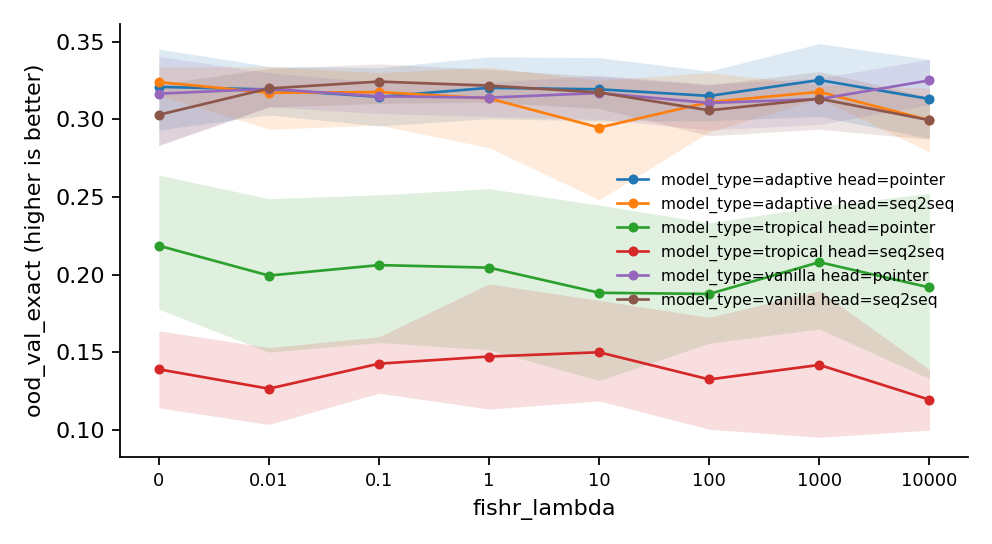
\includegraphics[width=\textwidth]{metric_ood_val_exact.png}
\caption{\texttt{ood\_val\_exact} against \texttt{fishr\_lambda}: the mean over seeds with a 95\% bootstrap CI, one line per combination of the other factors.}
\label{fig:ood_val_exact}
\end{figure}

{\small
\begin{longtable}{lllrlrrr}
\caption{\texttt{ood\_val\_exact} per cell: mean, 95\% bootstrap CI, SD, seeds, diverged runs.}\label{tab:summary-ood_val_exact}\\
\toprule
\texttt{model\_type} & \texttt{head} & \texttt{fishr\_lambda} & mean & 95\% CI & SD & $n$ & div.\\
\midrule
\endhead
adaptive & pointer & 0 & 0.321 & [0.293, 0.345] & 0.0322 & 5 & 0\\
adaptive & pointer & 0.01 & 0.3193 & [0.303, 0.334] & 0.0203 & 5 & 0\\
adaptive & pointer & 0.1 & 0.3145 & [0.296, 0.333] & 0.0251 & 5 & 0\\
adaptive & pointer & 1 & 0.3203 & [0.3, 0.34] & 0.0257 & 5 & 0\\
adaptive & pointer & 10 & 0.3194 & [0.299, 0.34] & 0.0268 & 5 & 0\\
adaptive & pointer & 100 & 0.3151 & [0.299, 0.331] & 0.0217 & 5 & 0\\
adaptive & pointer & 1000 & 0.3253 & [0.302, 0.349] & 0.0301 & 5 & 0\\
adaptive & pointer & 1e+04 & 0.3132 & [0.288, 0.339] & 0.0335 & 5 & 0\\
adaptive & seq2seq & 0 & 0.324 & [0.316, 0.334] & 0.0122 & 5 & 0\\
adaptive & seq2seq & 0.01 & 0.3172 & [0.294, 0.334] & 0.0266 & 5 & 0\\
adaptive & seq2seq & 0.1 & 0.3176 & [0.296, 0.33] & 0.0243 & 5 & 0\\
adaptive & seq2seq & 1 & 0.3135 & [0.282, 0.334] & 0.0344 & 5 & 0\\
adaptive & seq2seq & 10 & 0.2947 & [0.248, 0.325] & 0.052 & 5 & 0\\
adaptive & seq2seq & 100 & 0.3111 & [0.292, 0.33] & 0.025 & 5 & 0\\
adaptive & seq2seq & 1000 & 0.3177 & [0.313, 0.322] & 0.00557 & 5 & 0\\
adaptive & seq2seq & 1e+04 & 0.2995 & [0.279, 0.32] & 0.0269 & 5 & 0\\
tropical & pointer & 0 & 0.2187 & [0.178, 0.264] & 0.0568 & 5 & 0\\
tropical & pointer & 0.01 & 0.1994 & [0.15, 0.249] & 0.065 & 5 & 0\\
tropical & pointer & 0.1 & 0.2062 & [0.156, 0.251] & 0.0635 & 5 & 0\\
tropical & pointer & 1 & 0.2045 & [0.152, 0.255] & 0.0666 & 5 & 0\\
tropical & pointer & 10 & 0.1884 & [0.132, 0.245] & 0.0735 & 5 & 0\\
tropical & pointer & 100 & 0.1876 & [0.156, 0.233] & 0.0519 & 5 & 0\\
tropical & pointer & 1000 & 0.2081 & [0.165, 0.244] & 0.0514 & 5 & 0\\
tropical & pointer & 1e+04 & 0.1918 & [0.133, 0.252] & 0.0779 & 5 & 0\\
tropical & seq2seq & 0 & 0.1391 & [0.114, 0.164] & 0.0316 & 5 & 0\\
tropical & seq2seq & 0.01 & 0.1266 & [0.104, 0.153] & 0.0313 & 5 & 0\\
tropical & seq2seq & 0.1 & 0.1427 & [0.124, 0.16] & 0.0236 & 5 & 0\\
tropical & seq2seq & 1 & 0.1473 & [0.113, 0.194] & 0.052 & 5 & 0\\
tropical & seq2seq & 10 & 0.1501 & [0.119, 0.183] & 0.0412 & 5 & 0\\
tropical & seq2seq & 100 & 0.1326 & [0.1, 0.173] & 0.0454 & 5 & 0\\
tropical & seq2seq & 1000 & 0.1419 & [0.0953, 0.19] & 0.0613 & 5 & 0\\
tropical & seq2seq & 1e+04 & 0.1195 & [0.0999, 0.139] & 0.0256 & 5 & 0\\
vanilla & pointer & 0 & 0.3166 & [0.284, 0.341] & 0.0384 & 5 & 0\\
vanilla & pointer & 0.01 & 0.3197 & [0.308, 0.33] & 0.0147 & 5 & 0\\
vanilla & pointer & 0.1 & 0.3149 & [0.304, 0.324] & 0.013 & 5 & 0\\
vanilla & pointer & 1 & 0.314 & [0.302, 0.324] & 0.0138 & 5 & 0\\
vanilla & pointer & 10 & 0.317 & [0.3, 0.328] & 0.0194 & 5 & 0\\
vanilla & pointer & 100 & 0.3106 & [0.293, 0.323] & 0.0195 & 5 & 0\\
vanilla & pointer & 1000 & 0.3131 & [0.297, 0.327] & 0.0194 & 5 & 0\\
vanilla & pointer & 1e+04 & 0.3251 & [0.31, 0.339] & 0.0191 & 5 & 0\\
vanilla & seq2seq & 0 & 0.303 & [0.283, 0.323] & 0.0264 & 5 & 0\\
vanilla & seq2seq & 0.01 & 0.3199 & [0.308, 0.333] & 0.0158 & 5 & 0\\
vanilla & seq2seq & 0.1 & 0.3244 & [0.31, 0.336] & 0.016 & 5 & 0\\
vanilla & seq2seq & 1 & 0.3217 & [0.311, 0.332] & 0.0137 & 5 & 0\\
vanilla & seq2seq & 10 & 0.3173 & [0.307, 0.328] & 0.0138 & 5 & 0\\
vanilla & seq2seq & 100 & 0.3058 & [0.289, 0.322] & 0.0225 & 5 & 0\\
vanilla & seq2seq & 1000 & 0.3133 & [0.294, 0.331] & 0.0239 & 5 & 0\\
vanilla & seq2seq & 1e+04 & 0.2995 & [0.287, 0.314] & 0.0182 & 5 & 0\\
\bottomrule
\end{longtable}
}

{\small
\begin{longtable}{lllrrrl}
\caption{\texttt{ood\_val\_exact}: each level of \texttt{fishr\_lambda} against its control (0), within each combination of the other factors. parametric: Dunnett vs control.}\label{tab:control-ood_val_exact}\\
\toprule
\texttt{model\_type} & \texttt{head} & \texttt{fishr\_lambda} & difference & 95\% CI & $p$ & \\
\midrule
\endhead
adaptive & pointer & 0.01 & -0.00168 & [-0.0493, 0.046] & 1.0000 & \\
adaptive & pointer & 0.1 & -0.00642 & [-0.0541, 0.0412] & 0.9992 & \\
adaptive & pointer & 1 & $-6.200\times10^{-4}$ & [-0.0483, 0.047] & 1.0000 & \\
adaptive & pointer & 10 & -0.00158 & [-0.0492, 0.0461] & 1.0000 & \\
adaptive & pointer & 100 & -0.00584 & [-0.0535, 0.0418] & 0.9996 & \\
adaptive & pointer & 1000 & 0.00438 & [-0.0433, 0.052] & 0.9999 & \\
adaptive & pointer & 1e+04 & -0.0078 & [-0.0555, 0.0399] & 0.9975 & \\
adaptive & seq2seq & 0.01 & -0.00688 & [-0.0575, 0.0437] & 0.9992 & \\
adaptive & seq2seq & 0.1 & -0.00646 & [-0.0571, 0.0441] & 0.9995 & \\
adaptive & seq2seq & 1 & -0.0105 & [-0.0611, 0.0401] & 0.9898 & \\
adaptive & seq2seq & 10 & -0.0293 & [-0.0799, 0.0213] & 0.4523 & \\
adaptive & seq2seq & 100 & -0.01292 & [-0.0635, 0.0377] & 0.9692 & \\
adaptive & seq2seq & 1000 & -0.0063 & [-0.0569, 0.0443] & 0.9995 & \\
adaptive & seq2seq & 1e+04 & -0.02454 & [-0.0751, 0.0261] & 0.6308 & \\
tropical & pointer & 0.01 & -0.01924 & [-0.131, 0.0925] & 0.9966 & \\
tropical & pointer & 0.1 & -0.0125 & [-0.124, 0.0992] & 0.9998 & \\
tropical & pointer & 1 & -0.01414 & [-0.126, 0.0976] & 0.9995 & \\
tropical & pointer & 10 & -0.03032 & [-0.142, 0.0814] & 0.9584 & \\
tropical & pointer & 100 & -0.03106 & [-0.143, 0.0807] & 0.9532 & \\
tropical & pointer & 1000 & -0.0106 & [-0.122, 0.101] & 0.9999 & \\
tropical & pointer & 1e+04 & -0.0269 & [-0.139, 0.0848] & 0.9772 & \\
tropical & seq2seq & 0.01 & -0.0125 & [-0.084, 0.059] & 0.9962 & \\
tropical & seq2seq & 0.1 & 0.00362 & [-0.0679, 0.0751] & 1.0000 & \\
tropical & seq2seq & 1 & 0.00822 & [-0.0633, 0.0797] & 0.9997 & \\
tropical & seq2seq & 10 & 0.01096 & [-0.0606, 0.0825] & 0.9983 & \\
tropical & seq2seq & 100 & -0.00652 & [-0.078, 0.065] & 0.9999 & \\
tropical & seq2seq & 1000 & 0.00282 & [-0.0687, 0.0743] & 1.0000 & \\
tropical & seq2seq & 1e+04 & -0.0196 & [-0.0911, 0.0519] & 0.9564 & \\
vanilla & pointer & 0.01 & 0.00306 & [-0.0337, 0.0398] & 1.0000 & \\
vanilla & pointer & 0.1 & -0.00172 & [-0.0385, 0.035] & 1.0000 & \\
vanilla & pointer & 1 & -0.00258 & [-0.0393, 0.0342] & 1.0000 & \\
vanilla & pointer & 10 & $3.800\times10^{-4}$ & [-0.0364, 0.0371] & 1.0000 & \\
vanilla & pointer & 100 & -0.006 & [-0.0428, 0.0308] & 0.9975 & \\
vanilla & pointer & 1000 & -0.0035 & [-0.0403, 0.0333] & 0.9999 & \\
vanilla & pointer & 1e+04 & 0.00854 & [-0.0282, 0.0453] & 0.9811 & \\
vanilla & seq2seq & 0.01 & 0.01698 & [-0.0168, 0.0507] & 0.5950 & \\
vanilla & seq2seq & 0.1 & 0.0214 & [-0.0123, 0.0551] & 0.3601 & \\
vanilla & seq2seq & 1 & 0.01878 & [-0.015, 0.0525] & 0.4932 & \\
vanilla & seq2seq & 10 & 0.01438 & [-0.0194, 0.0481] & 0.7445 & \\
vanilla & seq2seq & 100 & 0.00286 & [-0.0309, 0.0366] & 1.0000 & \\
vanilla & seq2seq & 1000 & 0.01038 & [-0.0234, 0.0441] & 0.9255 & \\
vanilla & seq2seq & 1e+04 & -0.00344 & [-0.0372, 0.0303] & 0.9999 & \\
\bottomrule
\end{longtable}
}

{\small
\begin{longtable}{llrrrrr}
\caption{\texttt{ood\_val\_exact} against log10 \texttt{fishr\_lambda}: parametric: OLS slope t-test, seed-bootstrap CI, with the Jonckheere--Terpstra ordered-trend $\tau$ and $p$.}\label{tab:trend-ood_val_exact}\\
\toprule
\texttt{model\_type} & \texttt{head} & estimate & 95\% CI & $p$ & JT $\tau$ & JT $p$\\
\midrule
\endhead
adaptive & pointer & $-7.071\times10^{-5}$ & [-0.00231, 0.00226] & 0.9732 & -0.0019 & 1.0000\\
adaptive & seq2seq & -0.001967 & [-0.00457, $7.92\times10^{-4}$] & 0.4327 & -0.17 & 0.2038\\
tropical & pointer & -0.001289 & [-0.00725, 0.00304] & 0.8019 & -0.0362 & 0.7952\\
tropical & seq2seq & -0.001344 & [-0.00452, 0.00187] & 0.6947 & -0.099 & 0.4671\\
vanilla & pointer & $3.379\times10^{-4}$ & [-0.00102, 0.0017] & 0.8099 & 0.0648 & 0.6453\\
vanilla & seq2seq & -0.003544 & [-0.00692, -0.00118] & 0.0209 & -0.29 & 0.0340\\
\bottomrule
\end{longtable}
}

{\small
\begin{longtable}{lrrrl}
\caption{\texttt{ood\_val\_exact}: paired contrasts by seed, Holm-corrected across the cells. parametric: paired t-test by seed, Holm.}\label{tab:paired-ood_val_exact}\\
\toprule
contrast (within) & difference & 95\% CI & $p$ & \\
\midrule
\endhead
\stackcell{model\_type: tropical - vanilla\\\footnotesize head=pointer fishr\_lambda=0 } & -0.09792 & [-0.212, 0.0163] & 0.1478 & \\
\stackcell{model\_type: tropical - vanilla\\\footnotesize head=pointer fishr\_lambda=0.01 } & -0.1202 & [-0.215, -0.0252] & 0.1478 & \\
\stackcell{model\_type: tropical - vanilla\\\footnotesize head=pointer fishr\_lambda=0.1 } & -0.1087 & [-0.2, -0.0175] & 0.1478 & \\
\stackcell{model\_type: tropical - vanilla\\\footnotesize head=pointer fishr\_lambda=1 } & -0.1095 & [-0.206, -0.0131] & 0.1478 & \\
\stackcell{model\_type: tropical - vanilla\\\footnotesize head=pointer fishr\_lambda=10 } & -0.1286 & [-0.234, -0.0233] & 0.1478 & \\
\stackcell{model\_type: tropical - vanilla\\\footnotesize head=pointer fishr\_lambda=100 } & -0.123 & [-0.211, -0.0347] & 0.1444 & \\
\stackcell{model\_type: tropical - vanilla\\\footnotesize head=pointer fishr\_lambda=1000 } & -0.105 & [-0.184, -0.0262] & 0.1460 & \\
\stackcell{model\_type: tropical - vanilla\\\footnotesize head=pointer fishr\_lambda=1e+04 } & -0.1334 & [-0.251, -0.0158] & 0.1478 & \\
\stackcell{model\_type: tropical - vanilla\\\footnotesize head=seq2seq fishr\_lambda=0 } & -0.1639 & [-0.196, -0.132] & 0.0021 & *\\
\stackcell{model\_type: tropical - vanilla\\\footnotesize head=seq2seq fishr\_lambda=0.01 } & -0.1933 & [-0.241, -0.146] & 0.0045 & *\\
\stackcell{model\_type: tropical - vanilla\\\footnotesize head=seq2seq fishr\_lambda=0.1 } & -0.1816 & [-0.213, -0.151] & 0.0013 & *\\
\stackcell{model\_type: tropical - vanilla\\\footnotesize head=seq2seq fishr\_lambda=1 } & -0.1744 & [-0.235, -0.114] & 0.0142 & *\\
\stackcell{model\_type: tropical - vanilla\\\footnotesize head=seq2seq fishr\_lambda=10 } & -0.1673 & [-0.223, -0.112] & 0.0134 & *\\
\stackcell{model\_type: tropical - vanilla\\\footnotesize head=seq2seq fishr\_lambda=100 } & -0.1732 & [-0.242, -0.105] & 0.0193 & *\\
\stackcell{model\_type: tropical - vanilla\\\footnotesize head=seq2seq fishr\_lambda=1000 } & -0.1714 & [-0.236, -0.107] & 0.0183 & *\\
\stackcell{model\_type: tropical - vanilla\\\footnotesize head=seq2seq fishr\_lambda=1e+04 } & -0.18 & [-0.214, -0.146] & 0.0018 & *\\
\stackcell{model\_type: adaptive - vanilla\\\footnotesize head=pointer fishr\_lambda=0 } & 0.00436 & [-0.0525, 0.0612] & 1.0000 & \\
\stackcell{model\_type: adaptive - vanilla\\\footnotesize head=pointer fishr\_lambda=0.01 } & $-3.800\times10^{-4}$ & [-0.0346, 0.0339] & 1.0000 & \\
\stackcell{model\_type: adaptive - vanilla\\\footnotesize head=pointer fishr\_lambda=0.1 } & $-3.400\times10^{-4}$ & [-0.0263, 0.0257] & 1.0000 & \\
\stackcell{model\_type: adaptive - vanilla\\\footnotesize head=pointer fishr\_lambda=1 } & 0.00632 & [-0.025, 0.0377] & 1.0000 & \\
\stackcell{model\_type: adaptive - vanilla\\\footnotesize head=pointer fishr\_lambda=10 } & 0.0024 & [-0.0169, 0.0217] & 1.0000 & \\
\stackcell{model\_type: adaptive - vanilla\\\footnotesize head=pointer fishr\_lambda=100 } & 0.00452 & [-0.0191, 0.0281] & 1.0000 & \\
\stackcell{model\_type: adaptive - vanilla\\\footnotesize head=pointer fishr\_lambda=1000 } & 0.01224 & [-0.0301, 0.0546] & 1.0000 & \\
\stackcell{model\_type: adaptive - vanilla\\\footnotesize head=pointer fishr\_lambda=1e+04 } & -0.01198 & [-0.0409, 0.0169] & 1.0000 & \\
\stackcell{model\_type: adaptive - vanilla\\\footnotesize head=seq2seq fishr\_lambda=0 } & 0.02108 & [-0.0229, 0.0651] & 1.0000 & \\
\stackcell{model\_type: adaptive - vanilla\\\footnotesize head=seq2seq fishr\_lambda=0.01 } & -0.00278 & [-0.0335, 0.0279] & 1.0000 & \\
\stackcell{model\_type: adaptive - vanilla\\\footnotesize head=seq2seq fishr\_lambda=0.1 } & -0.00678 & [-0.0472, 0.0336] & 1.0000 & \\
\stackcell{model\_type: adaptive - vanilla\\\footnotesize head=seq2seq fishr\_lambda=1 } & -0.0082 & [-0.0549, 0.0385] & 1.0000 & \\
\stackcell{model\_type: adaptive - vanilla\\\footnotesize head=seq2seq fishr\_lambda=10 } & -0.0226 & [-0.0782, 0.033] & 1.0000 & \\
\stackcell{model\_type: adaptive - vanilla\\\footnotesize head=seq2seq fishr\_lambda=100 } & 0.0053 & [-0.04, 0.0506] & 1.0000 & \\
\stackcell{model\_type: adaptive - vanilla\\\footnotesize head=seq2seq fishr\_lambda=1000 } & 0.0044 & [-0.0316, 0.0404] & 1.0000 & \\
\stackcell{model\_type: adaptive - vanilla\\\footnotesize head=seq2seq fishr\_lambda=1e+04 } & $-2.000\times10^{-5}$ & [-0.0235, 0.0234] & 1.0000 & \\
\stackcell{head: pointer - seq2seq\\\footnotesize model\_type=adaptive fishr\_lambda=0 } & -0.00308 & [-0.0558, 0.0496] & 1.0000 & \\
\stackcell{head: pointer - seq2seq\\\footnotesize model\_type=adaptive fishr\_lambda=0.01 } & 0.00212 & [-0.0515, 0.0557] & 1.0000 & \\
\stackcell{head: pointer - seq2seq\\\footnotesize model\_type=adaptive fishr\_lambda=0.1 } & -0.00304 & [-0.0549, 0.0488] & 1.0000 & \\
\stackcell{head: pointer - seq2seq\\\footnotesize model\_type=adaptive fishr\_lambda=1 } & 0.0068 & [-0.0547, 0.0683] & 1.0000 & \\
\stackcell{head: pointer - seq2seq\\\footnotesize model\_type=adaptive fishr\_lambda=10 } & 0.02464 & [-0.0572, 0.106] & 1.0000 & \\
\stackcell{head: pointer - seq2seq\\\footnotesize model\_type=adaptive fishr\_lambda=100 } & 0.004 & [-0.0452, 0.0532] & 1.0000 & \\
\stackcell{head: pointer - seq2seq\\\footnotesize model\_type=adaptive fishr\_lambda=1000 } & 0.0076 & [-0.0358, 0.051] & 1.0000 & \\
\stackcell{head: pointer - seq2seq\\\footnotesize model\_type=adaptive fishr\_lambda=1e+04 } & 0.01366 & [-0.0206, 0.0479] & 1.0000 & \\
\stackcell{head: pointer - seq2seq\\\footnotesize model\_type=tropical fishr\_lambda=0 } & 0.07958 & [-0.0227, 0.182] & 1.0000 & \\
\stackcell{head: pointer - seq2seq\\\footnotesize model\_type=tropical fishr\_lambda=0.01 } & 0.07284 & [-0.0237, 0.169] & 1.0000 & \\
\stackcell{head: pointer - seq2seq\\\footnotesize model\_type=tropical fishr\_lambda=0.1 } & 0.06346 & [-0.0172, 0.144] & 1.0000 & \\
\stackcell{head: pointer - seq2seq\\\footnotesize model\_type=tropical fishr\_lambda=1 } & 0.05722 & [-0.0744, 0.189] & 1.0000 & \\
\stackcell{head: pointer - seq2seq\\\footnotesize model\_type=tropical fishr\_lambda=10 } & 0.0383 & [-0.0229, 0.0995] & 1.0000 & \\
\stackcell{head: pointer - seq2seq\\\footnotesize model\_type=tropical fishr\_lambda=100 } & 0.05504 & [-0.0331, 0.143] & 1.0000 & \\
\stackcell{head: pointer - seq2seq\\\footnotesize model\_type=tropical fishr\_lambda=1000 } & 0.06616 & [-0.0359, 0.168] & 1.0000 & \\
\stackcell{head: pointer - seq2seq\\\footnotesize model\_type=tropical fishr\_lambda=1e+04 } & 0.07228 & [-0.0463, 0.191] & 1.0000 & \\
\stackcell{head: pointer - seq2seq\\\footnotesize model\_type=vanilla fishr\_lambda=0 } & 0.01364 & [-0.0543, 0.0816] & 1.0000 & \\
\stackcell{head: pointer - seq2seq\\\footnotesize model\_type=vanilla fishr\_lambda=0.01 } & $-2.800\times10^{-4}$ & [-0.00852, 0.00796] & 1.0000 & \\
\stackcell{head: pointer - seq2seq\\\footnotesize model\_type=vanilla fishr\_lambda=0.1 } & -0.00948 & [-0.0147, -0.00429] & 0.1715 & \\
\stackcell{head: pointer - seq2seq\\\footnotesize model\_type=vanilla fishr\_lambda=1 } & -0.00772 & [-0.0121, -0.00335] & 0.1849 & \\
\stackcell{head: pointer - seq2seq\\\footnotesize model\_type=vanilla fishr\_lambda=10 } & $-3.600\times10^{-4}$ & [-0.0236, 0.0229] & 1.0000 & \\
\stackcell{head: pointer - seq2seq\\\footnotesize model\_type=vanilla fishr\_lambda=100 } & 0.00478 & [-0.0256, 0.0351] & 1.0000 & \\
\stackcell{head: pointer - seq2seq\\\footnotesize model\_type=vanilla fishr\_lambda=1000 } & $-2.400\times10^{-4}$ & [-0.0359, 0.0355] & 1.0000 & \\
\stackcell{head: pointer - seq2seq\\\footnotesize model\_type=vanilla fishr\_lambda=1e+04 } & 0.02562 & [-0.00431, 0.0555] & 1.0000 & \\
\bottomrule
\end{longtable}
}

\subsection{\texttt{ood\_noise\_f1}}
\begin{figure}[tbp]
\centering
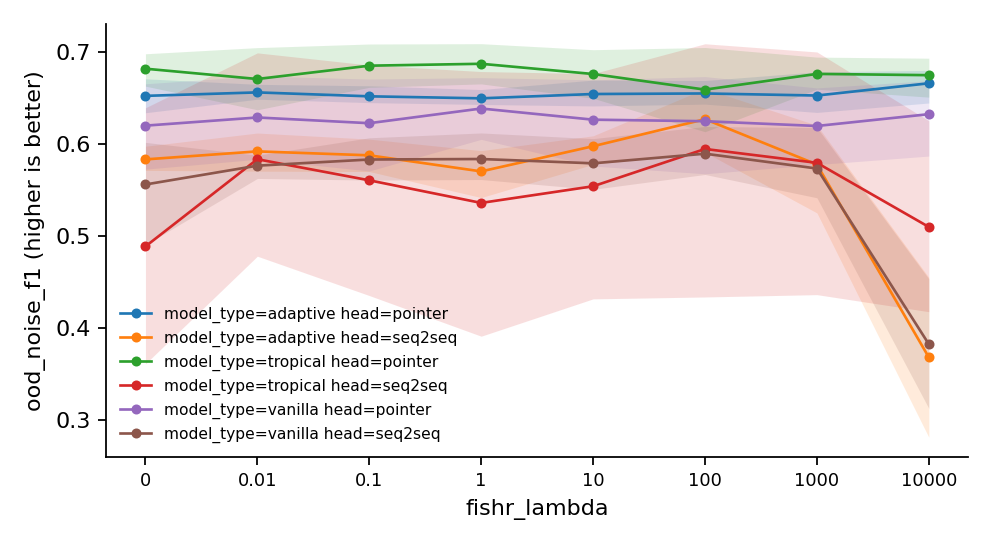
\includegraphics[width=\textwidth]{metric_ood_noise_f1.png}
\caption{\texttt{ood\_noise\_f1} against \texttt{fishr\_lambda}: the mean over seeds with a 95\% bootstrap CI, one line per combination of the other factors.}
\label{fig:ood_noise_f1}
\end{figure}

{\small
\begin{longtable}{lllrlrrr}
\caption{\texttt{ood\_noise\_f1} per cell: mean, 95\% bootstrap CI, SD, seeds, diverged runs.}\label{tab:summary-ood_noise_f1}\\
\toprule
\texttt{model\_type} & \texttt{head} & \texttt{fishr\_lambda} & mean & 95\% CI & SD & $n$ & div.\\
\midrule
\endhead
adaptive & pointer & 0 & 0.6519 & [0.634, 0.67] & 0.0241 & 5 & 0\\
adaptive & pointer & 0.01 & 0.6557 & [0.648, 0.664] & 0.0102 & 5 & 0\\
adaptive & pointer & 0.1 & 0.6514 & [0.645, 0.663] & 0.0129 & 5 & 0\\
adaptive & pointer & 1 & 0.6492 & [0.643, 0.659] & 0.0109 & 5 & 0\\
adaptive & pointer & 10 & 0.6539 & [0.641, 0.669] & 0.0175 & 5 & 0\\
adaptive & pointer & 100 & 0.6545 & [0.643, 0.669] & 0.0156 & 5 & 0\\
adaptive & pointer & 1000 & 0.6523 & [0.634, 0.678] & 0.0288 & 5 & 0\\
adaptive & pointer & 1e+04 & 0.6656 & [0.644, 0.68] & 0.0238 & 5 & 0\\
adaptive & seq2seq & 0 & 0.583 & [0.571, 0.597] & 0.0171 & 5 & 0\\
adaptive & seq2seq & 0.01 & 0.5916 & [0.57, 0.612] & 0.0271 & 5 & 0\\
adaptive & seq2seq & 0.1 & 0.5874 & [0.57, 0.605] & 0.0234 & 5 & 0\\
adaptive & seq2seq & 1 & 0.5699 & [0.542, 0.592] & 0.0336 & 5 & 0\\
adaptive & seq2seq & 10 & 0.5972 & [0.578, 0.609] & 0.022 & 5 & 0\\
adaptive & seq2seq & 100 & 0.6266 & [0.591, 0.66] & 0.0448 & 5 & 0\\
adaptive & seq2seq & 1000 & 0.5774 & [0.525, 0.62] & 0.0618 & 5 & 0\\
adaptive & seq2seq & 1e+04 & 0.3681 & [0.281, 0.455] & 0.11 & 5 & 0\\
tropical & pointer & 0 & 0.6814 & [0.662, 0.698] & 0.0225 & 5 & 0\\
tropical & pointer & 0.01 & 0.6702 & [0.637, 0.704] & 0.0436 & 5 & 0\\
tropical & pointer & 0.1 & 0.6847 & [0.661, 0.708] & 0.0309 & 5 & 0\\
tropical & pointer & 1 & 0.6867 & [0.665, 0.709] & 0.0283 & 5 & 0\\
tropical & pointer & 10 & 0.6756 & [0.649, 0.702] & 0.0352 & 5 & 0\\
tropical & pointer & 100 & 0.6587 & [0.613, 0.704] & 0.0587 & 5 & 0\\
tropical & pointer & 1000 & 0.6757 & [0.659, 0.694] & 0.0227 & 5 & 0\\
tropical & pointer & 1e+04 & 0.6744 & [0.651, 0.693] & 0.0279 & 5 & 0\\
tropical & seq2seq & 0 & 0.4885 & [0.361, 0.639] & 0.172 & 5 & 0\\
tropical & seq2seq & 0.01 & 0.5831 & [0.478, 0.699] & 0.138 & 5 & 0\\
tropical & seq2seq & 0.1 & 0.5602 & [0.435, 0.685] & 0.16 & 5 & 0\\
tropical & seq2seq & 1 & 0.5357 & [0.391, 0.678] & 0.198 & 5 & 0\\
tropical & seq2seq & 10 & 0.5538 & [0.432, 0.676] & 0.159 & 5 & 0\\
tropical & seq2seq & 100 & 0.5943 & [0.434, 0.708] & 0.191 & 5 & 0\\
tropical & seq2seq & 1000 & 0.5792 & [0.436, 0.7] & 0.168 & 5 & 0\\
tropical & seq2seq & 1e+04 & 0.5096 & [0.418, 0.625] & 0.134 & 5 & 0\\
vanilla & pointer & 0 & 0.6196 & [0.572, 0.665] & 0.0597 & 5 & 0\\
vanilla & pointer & 0.01 & 0.6284 & [0.583, 0.673] & 0.0628 & 5 & 0\\
vanilla & pointer & 0.1 & 0.6222 & [0.57, 0.67] & 0.0634 & 5 & 0\\
vanilla & pointer & 1 & 0.6382 & [0.605, 0.672] & 0.0428 & 5 & 0\\
vanilla & pointer & 10 & 0.6261 & [0.576, 0.669] & 0.0608 & 5 & 0\\
vanilla & pointer & 100 & 0.6244 & [0.567, 0.673] & 0.0671 & 5 & 0\\
vanilla & pointer & 1000 & 0.6192 & [0.577, 0.661] & 0.0544 & 5 & 0\\
vanilla & pointer & 1e+04 & 0.632 & [0.587, 0.668] & 0.0501 & 5 & 0\\
vanilla & seq2seq & 0 & 0.5557 & [0.49, 0.601] & 0.0748 & 5 & 0\\
vanilla & seq2seq & 0.01 & 0.5761 & [0.562, 0.587] & 0.0158 & 5 & 0\\
vanilla & seq2seq & 0.1 & 0.5828 & [0.561, 0.606] & 0.029 & 5 & 0\\
vanilla & seq2seq & 1 & 0.5834 & [0.561, 0.612] & 0.0321 & 5 & 0\\
vanilla & seq2seq & 10 & 0.5787 & [0.55, 0.605] & 0.0346 & 5 & 0\\
vanilla & seq2seq & 100 & 0.5892 & [0.567, 0.619] & 0.0338 & 5 & 0\\
vanilla & seq2seq & 1000 & 0.5731 & [0.541, 0.617] & 0.0518 & 5 & 0\\
vanilla & seq2seq & 1e+04 & 0.3824 & [0.313, 0.453] & 0.0936 & 5 & 0\\
\bottomrule
\end{longtable}
}

{\small
\begin{longtable}{lllrrrl}
\caption{\texttt{ood\_noise\_f1}: each level of \texttt{fishr\_lambda} against its control (0), within each combination of the other factors. parametric: Dunnett vs control.}\label{tab:control-ood_noise_f1}\\
\toprule
\texttt{model\_type} & \texttt{head} & \texttt{fishr\_lambda} & difference & 95\% CI & $p$ & \\
\midrule
\endhead
adaptive & pointer & 0.01 & 0.003766 & [-0.0296, 0.0371] & 0.9998 & \\
adaptive & pointer & 0.1 & $-4.889\times10^{-4}$ & [-0.0338, 0.0329] & 1.0000 & \\
adaptive & pointer & 1 & -0.002664 & [-0.036, 0.0307] & 1.0000 & \\
adaptive & pointer & 10 & 0.002013 & [-0.0313, 0.0354] & 1.0000 & \\
adaptive & pointer & 100 & 0.002612 & [-0.0307, 0.036] & 1.0000 & \\
adaptive & pointer & 1000 & $3.760\times10^{-4}$ & [-0.033, 0.0337] & 1.0000 & \\
adaptive & pointer & 1e+04 & 0.01367 & [-0.0197, 0.047] & 0.7745 & \\
adaptive & seq2seq & 0.01 & 0.008691 & [-0.0808, 0.0982] & 0.9999 & \\
adaptive & seq2seq & 0.1 & 0.00442 & [-0.0851, 0.0939] & 1.0000 & \\
adaptive & seq2seq & 1 & -0.01303 & [-0.103, 0.0765] & 0.9988 & \\
adaptive & seq2seq & 10 & 0.0143 & [-0.0752, 0.104] & 0.9978 & \\
adaptive & seq2seq & 100 & 0.04361 & [-0.0459, 0.133] & 0.6262 & \\
adaptive & seq2seq & 1000 & -0.00556 & [-0.0951, 0.0839] & 1.0000 & \\
adaptive & seq2seq & 1e+04 & -0.2148 & [-0.304, -0.125] & $<10^{-4}$ & *\\
tropical & pointer & 0.01 & -0.01119 & [-0.0734, 0.051] & 0.9955 & \\
tropical & pointer & 0.1 & 0.003271 & [-0.0589, 0.0655] & 1.0000 & \\
tropical & pointer & 1 & 0.00533 & [-0.0569, 0.0675] & 1.0000 & \\
tropical & pointer & 10 & -0.00577 & [-0.068, 0.0564] & 0.9999 & \\
tropical & pointer & 100 & -0.02271 & [-0.0849, 0.0395] & 0.8496 & \\
tropical & pointer & 1000 & -0.005648 & [-0.0678, 0.0565] & 0.9999 & \\
tropical & pointer & 1e+04 & -0.007029 & [-0.0692, 0.0552] & 0.9998 & \\
tropical & seq2seq & 0.01 & 0.09466 & [-0.196, 0.385] & 0.9043 & \\
tropical & seq2seq & 0.1 & 0.07179 & [-0.219, 0.362] & 0.9739 & \\
tropical & seq2seq & 1 & 0.04726 & [-0.243, 0.338] & 0.9976 & \\
tropical & seq2seq & 10 & 0.06534 & [-0.225, 0.356] & 0.9841 & \\
tropical & seq2seq & 100 & 0.1058 & [-0.185, 0.396] & 0.8510 & \\
tropical & seq2seq & 1000 & 0.09076 & [-0.2, 0.381] & 0.9201 & \\
tropical & seq2seq & 1e+04 & 0.02117 & [-0.269, 0.312] & 1.0000 & \\
vanilla & pointer & 0.01 & 0.008854 & [-0.0927, 0.11] & 1.0000 & \\
vanilla & pointer & 0.1 & 0.002653 & [-0.0989, 0.104] & 1.0000 & \\
vanilla & pointer & 1 & 0.01859 & [-0.083, 0.12] & 0.9950 & \\
vanilla & pointer & 10 & 0.006473 & [-0.0951, 0.108] & 1.0000 & \\
vanilla & pointer & 100 & 0.004796 & [-0.0967, 0.106] & 1.0000 & \\
vanilla & pointer & 1000 & $-3.701\times10^{-4}$ & [-0.102, 0.101] & 1.0000 & \\
vanilla & pointer & 1e+04 & 0.01244 & [-0.0891, 0.114] & 0.9996 & \\
vanilla & seq2seq & 0.01 & 0.02043 & [-0.0701, 0.111] & 0.9839 & \\
vanilla & seq2seq & 0.1 & 0.02711 & [-0.0634, 0.118] & 0.9340 & \\
vanilla & seq2seq & 1 & 0.02765 & [-0.0629, 0.118] & 0.9278 & \\
vanilla & seq2seq & 10 & 0.02298 & [-0.0676, 0.114] & 0.9701 & \\
vanilla & seq2seq & 100 & 0.03344 & [-0.0571, 0.124] & 0.8432 & \\
vanilla & seq2seq & 1000 & 0.01734 & [-0.0732, 0.108] & 0.9936 & \\
vanilla & seq2seq & 1e+04 & -0.1733 & [-0.264, -0.0828] & $<10^{-4}$ & *\\
\bottomrule
\end{longtable}
}

{\small
\begin{longtable}{llrrrrr}
\caption{\texttt{ood\_noise\_f1} against log10 \texttt{fishr\_lambda}: parametric: OLS slope t-test, seed-bootstrap CI, with the Jonckheere--Terpstra ordered-trend $\tau$ and $p$.}\label{tab:trend-ood_noise_f1}\\
\toprule
\texttt{model\_type} & \texttt{head} & estimate & 95\% CI & $p$ & JT $\tau$ & JT $p$\\
\midrule
\endhead
adaptive & pointer & 0.001311 & [-0.00136, 0.00337] & 0.3776 & 0.059 & 0.6703\\
adaptive & seq2seq & -0.02264 & [-0.0337, -0.0116] & 0.0032 & -0.192 & 0.1494\\
tropical & pointer & -0.001192 & [-0.00392, 0.00241] & 0.6913 & -0.059 & 0.6753\\
tropical & seq2seq & -0.004428 & [-0.00748, -0.00138] & 0.7370 & -0.0476 & 0.7261\\
vanilla & pointer & $-3.243\times10^{-4}$ & [-0.00321, 0.00317] & 0.9435 & -0.0133 & 0.9346\\
vanilla & seq2seq & -0.02125 & [-0.0287, -0.0138] & 0.0013 & -0.387 & 0.0026\\
\bottomrule
\end{longtable}
}

{\small
\begin{longtable}{lrrrl}
\caption{\texttt{ood\_noise\_f1}: paired contrasts by seed, Holm-corrected across the cells. parametric: paired t-test by seed, Holm.}\label{tab:paired-ood_noise_f1}\\
\toprule
contrast (within) & difference & 95\% CI & $p$ & \\
\midrule
\endhead
\stackcell{model\_type: tropical - vanilla\\\footnotesize head=pointer fishr\_lambda=0 } & 0.0618 & [0.00317, 0.12] & 0.6874 & \\
\stackcell{model\_type: tropical - vanilla\\\footnotesize head=pointer fishr\_lambda=0.01 } & 0.04176 & [-0.0591, 0.143] & 1.0000 & \\
\stackcell{model\_type: tropical - vanilla\\\footnotesize head=pointer fishr\_lambda=0.1 } & 0.06242 & [-0.0276, 0.152] & 1.0000 & \\
\stackcell{model\_type: tropical - vanilla\\\footnotesize head=pointer fishr\_lambda=1 } & 0.04854 & [-0.0252, 0.122] & 1.0000 & \\
\stackcell{model\_type: tropical - vanilla\\\footnotesize head=pointer fishr\_lambda=10 } & 0.04956 & [-0.0345, 0.134] & 1.0000 & \\
\stackcell{model\_type: tropical - vanilla\\\footnotesize head=pointer fishr\_lambda=100 } & 0.0343 & [-0.0593, 0.128] & 1.0000 & \\
\stackcell{model\_type: tropical - vanilla\\\footnotesize head=pointer fishr\_lambda=1000 } & 0.05653 & [-0.00631, 0.119] & 1.0000 & \\
\stackcell{model\_type: tropical - vanilla\\\footnotesize head=pointer fishr\_lambda=1e+04 } & 0.04233 & [-0.0418, 0.127] & 1.0000 & \\
\stackcell{model\_type: tropical - vanilla\\\footnotesize head=seq2seq fishr\_lambda=0 } & -0.06726 & [-0.275, 0.14] & 1.0000 & \\
\stackcell{model\_type: tropical - vanilla\\\footnotesize head=seq2seq fishr\_lambda=0.01 } & 0.006979 & [-0.173, 0.187] & 1.0000 & \\
\stackcell{model\_type: tropical - vanilla\\\footnotesize head=seq2seq fishr\_lambda=0.1 } & -0.02257 & [-0.229, 0.184] & 1.0000 & \\
\stackcell{model\_type: tropical - vanilla\\\footnotesize head=seq2seq fishr\_lambda=1 } & -0.04765 & [-0.307, 0.211] & 1.0000 & \\
\stackcell{model\_type: tropical - vanilla\\\footnotesize head=seq2seq fishr\_lambda=10 } & -0.0249 & [-0.235, 0.185] & 1.0000 & \\
\stackcell{model\_type: tropical - vanilla\\\footnotesize head=seq2seq fishr\_lambda=100 } & 0.005107 & [-0.24, 0.25] & 1.0000 & \\
\stackcell{model\_type: tropical - vanilla\\\footnotesize head=seq2seq fishr\_lambda=1000 } & 0.006172 & [-0.175, 0.187] & 1.0000 & \\
\stackcell{model\_type: tropical - vanilla\\\footnotesize head=seq2seq fishr\_lambda=1e+04 } & 0.1272 & [-0.104, 0.358] & 1.0000 & \\
\stackcell{model\_type: adaptive - vanilla\\\footnotesize head=pointer fishr\_lambda=0 } & 0.03231 & [-0.0414, 0.106] & 1.0000 & \\
\stackcell{model\_type: adaptive - vanilla\\\footnotesize head=pointer fishr\_lambda=0.01 } & 0.02722 & [-0.059, 0.113] & 1.0000 & \\
\stackcell{model\_type: adaptive - vanilla\\\footnotesize head=pointer fishr\_lambda=0.1 } & 0.02917 & [-0.0633, 0.122] & 1.0000 & \\
\stackcell{model\_type: adaptive - vanilla\\\footnotesize head=pointer fishr\_lambda=1 } & 0.01106 & [-0.0483, 0.0704] & 1.0000 & \\
\stackcell{model\_type: adaptive - vanilla\\\footnotesize head=pointer fishr\_lambda=10 } & 0.02785 & [-0.0631, 0.119] & 1.0000 & \\
\stackcell{model\_type: adaptive - vanilla\\\footnotesize head=pointer fishr\_lambda=100 } & 0.03013 & [-0.0683, 0.129] & 1.0000 & \\
\stackcell{model\_type: adaptive - vanilla\\\footnotesize head=pointer fishr\_lambda=1000 } & 0.03306 & [-0.0546, 0.121] & 1.0000 & \\
\stackcell{model\_type: adaptive - vanilla\\\footnotesize head=pointer fishr\_lambda=1e+04 } & 0.03354 & [-0.0101, 0.0772] & 1.0000 & \\
\stackcell{model\_type: adaptive - vanilla\\\footnotesize head=seq2seq fishr\_lambda=0 } & 0.02724 & [-0.0857, 0.14] & 1.0000 & \\
\stackcell{model\_type: adaptive - vanilla\\\footnotesize head=seq2seq fishr\_lambda=0.01 } & 0.0155 & [-0.0327, 0.0637] & 1.0000 & \\
\stackcell{model\_type: adaptive - vanilla\\\footnotesize head=seq2seq fishr\_lambda=0.1 } & 0.004545 & [-0.0499, 0.059] & 1.0000 & \\
\stackcell{model\_type: adaptive - vanilla\\\footnotesize head=seq2seq fishr\_lambda=1 } & -0.01344 & [-0.0897, 0.0628] & 1.0000 & \\
\stackcell{model\_type: adaptive - vanilla\\\footnotesize head=seq2seq fishr\_lambda=10 } & 0.01856 & [-0.0292, 0.0664] & 1.0000 & \\
\stackcell{model\_type: adaptive - vanilla\\\footnotesize head=seq2seq fishr\_lambda=100 } & 0.03741 & [-0.027, 0.102] & 1.0000 & \\
\stackcell{model\_type: adaptive - vanilla\\\footnotesize head=seq2seq fishr\_lambda=1000 } & 0.00434 & [-0.0685, 0.0771] & 1.0000 & \\
\stackcell{model\_type: adaptive - vanilla\\\footnotesize head=seq2seq fishr\_lambda=1e+04 } & -0.0143 & [-0.0972, 0.0686] & 1.0000 & \\
\stackcell{head: pointer - seq2seq\\\footnotesize model\_type=adaptive fishr\_lambda=0 } & 0.06894 & [0.0351, 0.103] & 0.1139 & \\
\stackcell{head: pointer - seq2seq\\\footnotesize model\_type=adaptive fishr\_lambda=0.01 } & 0.06402 & [0.0327, 0.0953] & 0.1139 & \\
\stackcell{head: pointer - seq2seq\\\footnotesize model\_type=adaptive fishr\_lambda=0.1 } & 0.06403 & [0.0325, 0.0956] & 0.1139 & \\
\stackcell{head: pointer - seq2seq\\\footnotesize model\_type=adaptive fishr\_lambda=1 } & 0.0793 & [0.0394, 0.119] & 0.1139 & \\
\stackcell{head: pointer - seq2seq\\\footnotesize model\_type=adaptive fishr\_lambda=10 } & 0.05666 & [0.0267, 0.0866] & 0.1189 & \\
\stackcell{head: pointer - seq2seq\\\footnotesize model\_type=adaptive fishr\_lambda=100 } & 0.02795 & [-0.0236, 0.0795] & 1.0000 & \\
\stackcell{head: pointer - seq2seq\\\footnotesize model\_type=adaptive fishr\_lambda=1000 } & 0.07488 & [-0.0069, 0.157] & 0.9576 & \\
\stackcell{head: pointer - seq2seq\\\footnotesize model\_type=adaptive fishr\_lambda=1e+04 } & 0.2974 & [0.144, 0.451] & 0.1163 & \\
\stackcell{head: pointer - seq2seq\\\footnotesize model\_type=tropical fishr\_lambda=0 } & 0.1929 & [-0.0312, 0.417] & 0.9773 & \\
\stackcell{head: pointer - seq2seq\\\footnotesize model\_type=tropical fishr\_lambda=0.01 } & 0.08707 & [-0.12, 0.294] & 1.0000 & \\
\stackcell{head: pointer - seq2seq\\\footnotesize model\_type=tropical fishr\_lambda=0.1 } & 0.1244 & [-0.0909, 0.34] & 1.0000 & \\
\stackcell{head: pointer - seq2seq\\\footnotesize model\_type=tropical fishr\_lambda=1 } & 0.151 & [-0.0988, 0.401] & 1.0000 & \\
\stackcell{head: pointer - seq2seq\\\footnotesize model\_type=tropical fishr\_lambda=10 } & 0.1218 & [-0.105, 0.349] & 1.0000 & \\
\stackcell{head: pointer - seq2seq\\\footnotesize model\_type=tropical fishr\_lambda=100 } & 0.06442 & [-0.211, 0.34] & 1.0000 & \\
\stackcell{head: pointer - seq2seq\\\footnotesize model\_type=tropical fishr\_lambda=1000 } & 0.09652 & [-0.13, 0.323] & 1.0000 & \\
\stackcell{head: pointer - seq2seq\\\footnotesize model\_type=tropical fishr\_lambda=1e+04 } & 0.1647 & [-0.0107, 0.34] & 0.9537 & \\
\stackcell{head: pointer - seq2seq\\\footnotesize model\_type=vanilla fishr\_lambda=0 } & 0.06387 & [-0.0782, 0.206] & 1.0000 & \\
\stackcell{head: pointer - seq2seq\\\footnotesize model\_type=vanilla fishr\_lambda=0.01 } & 0.05229 & [-0.0108, 0.115] & 0.9940 & \\
\stackcell{head: pointer - seq2seq\\\footnotesize model\_type=vanilla fishr\_lambda=0.1 } & 0.03941 & [-0.0262, 0.105] & 1.0000 & \\
\stackcell{head: pointer - seq2seq\\\footnotesize model\_type=vanilla fishr\_lambda=1 } & 0.0548 & [$-2.42\times10^{-4}$, 0.11] & 0.8607 & \\
\stackcell{head: pointer - seq2seq\\\footnotesize model\_type=vanilla fishr\_lambda=10 } & 0.04736 & [-0.00583, 0.101] & 0.9631 & \\
\stackcell{head: pointer - seq2seq\\\footnotesize model\_type=vanilla fishr\_lambda=100 } & 0.03523 & [-0.039, 0.109] & 1.0000 & \\
\stackcell{head: pointer - seq2seq\\\footnotesize model\_type=vanilla fishr\_lambda=1000 } & 0.04616 & [-0.064, 0.156] & 1.0000 & \\
\stackcell{head: pointer - seq2seq\\\footnotesize model\_type=vanilla fishr\_lambda=1e+04 } & 0.2496 & [0.106, 0.393] & 0.1527 & \\
\bottomrule
\end{longtable}
}

\subsection{\texttt{ood\_noise\_exact}}
\begin{figure}[tbp]
\centering
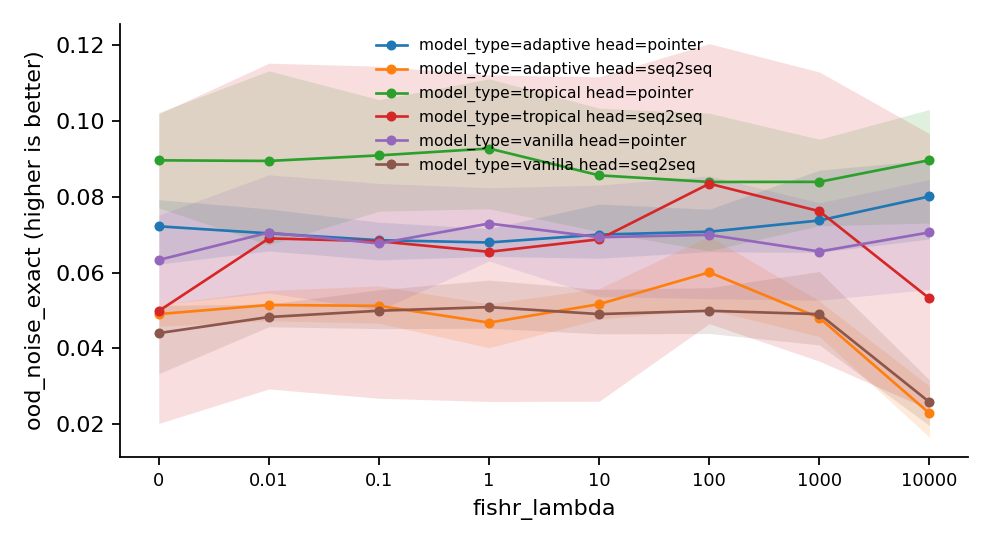
\includegraphics[width=\textwidth]{metric_ood_noise_exact.png}
\caption{\texttt{ood\_noise\_exact} against \texttt{fishr\_lambda}: the mean over seeds with a 95\% bootstrap CI, one line per combination of the other factors.}
\label{fig:ood_noise_exact}
\end{figure}

{\small
\begin{longtable}{lllrlrrr}
\caption{\texttt{ood\_noise\_exact} per cell: mean, 95\% bootstrap CI, SD, seeds, diverged runs.}\label{tab:summary-ood_noise_exact}\\
\toprule
\texttt{model\_type} & \texttt{head} & \texttt{fishr\_lambda} & mean & 95\% CI & SD & $n$ & div.\\
\midrule
\endhead
adaptive & pointer & 0 & 0.07218 & [0.0622, 0.0792] & 0.0111 & 5 & 0\\
adaptive & pointer & 0.01 & 0.07032 & [0.0657, 0.0768] & 0.00735 & 5 & 0\\
adaptive & pointer & 0.1 & 0.06852 & [0.0633, 0.0733] & 0.00627 & 5 & 0\\
adaptive & pointer & 1 & 0.06792 & [0.0642, 0.0716] & 0.00476 & 5 & 0\\
adaptive & pointer & 10 & 0.07 & [0.0638, 0.0781] & 0.00901 & 5 & 0\\
adaptive & pointer & 100 & 0.07076 & [0.0655, 0.0767] & 0.00722 & 5 & 0\\
adaptive & pointer & 1000 & 0.07372 & [0.0653, 0.087] & 0.0144 & 5 & 0\\
adaptive & pointer & 1e+04 & 0.08006 & [0.0688, 0.0896] & 0.014 & 5 & 0\\
adaptive & seq2seq & 0 & 0.04904 & [0.0458, 0.0515] & 0.00381 & 5 & 0\\
adaptive & seq2seq & 0.01 & 0.05144 & [0.0473, 0.0553] & 0.00525 & 5 & 0\\
adaptive & seq2seq & 0.1 & 0.0512 & [0.0466, 0.0565] & 0.00629 & 5 & 0\\
adaptive & seq2seq & 1 & 0.04678 & [0.0402, 0.0518] & 0.00732 & 5 & 0\\
adaptive & seq2seq & 10 & 0.05166 & [0.0477, 0.0558] & 0.00526 & 5 & 0\\
adaptive & seq2seq & 100 & 0.06006 & [0.0503, 0.0696] & 0.0129 & 5 & 0\\
adaptive & seq2seq & 1000 & 0.04806 & [0.0431, 0.0525] & 0.00597 & 5 & 0\\
adaptive & seq2seq & 1e+04 & 0.02288 & [0.0166, 0.03] & 0.0088 & 5 & 0\\
tropical & pointer & 0 & 0.08958 & [0.077, 0.102] & 0.0159 & 5 & 0\\
tropical & pointer & 0.01 & 0.08942 & [0.0673, 0.113] & 0.0299 & 5 & 0\\
tropical & pointer & 0.1 & 0.09088 & [0.0762, 0.106] & 0.0188 & 5 & 0\\
tropical & pointer & 1 & 0.0927 & [0.0768, 0.111] & 0.023 & 5 & 0\\
tropical & pointer & 10 & 0.08562 & [0.0708, 0.103] & 0.0212 & 5 & 0\\
tropical & pointer & 100 & 0.08388 & [0.0658, 0.102] & 0.0249 & 5 & 0\\
tropical & pointer & 1000 & 0.0839 & [0.0723, 0.0951] & 0.0146 & 5 & 0\\
tropical & pointer & 1e+04 & 0.08964 & [0.073, 0.103] & 0.0191 & 5 & 0\\
tropical & seq2seq & 0 & 0.04986 & [0.0202, 0.102] & 0.0573 & 5 & 0\\
tropical & seq2seq & 0.01 & 0.069 & [0.0293, 0.115] & 0.0544 & 5 & 0\\
tropical & seq2seq & 0.1 & 0.06824 & [0.0268, 0.114] & 0.0559 & 5 & 0\\
tropical & seq2seq & 1 & 0.06546 & [0.026, 0.112] & 0.056 & 5 & 0\\
tropical & seq2seq & 10 & 0.06876 & [0.0261, 0.112] & 0.0594 & 5 & 0\\
tropical & seq2seq & 100 & 0.08342 & [0.0465, 0.12] & 0.0506 & 5 & 0\\
tropical & seq2seq & 1000 & 0.07616 & [0.0366, 0.113] & 0.0501 & 5 & 0\\
tropical & seq2seq & 1e+04 & 0.05316 & [0.0239, 0.0966] & 0.0482 & 5 & 0\\
vanilla & pointer & 0 & 0.06332 & [0.0515, 0.0751] & 0.0155 & 5 & 0\\
vanilla & pointer & 0.01 & 0.07054 & [0.0546, 0.0857] & 0.0208 & 5 & 0\\
vanilla & pointer & 0.1 & 0.06766 & [0.0501, 0.0835] & 0.0214 & 5 & 0\\
vanilla & pointer & 1 & 0.07292 & [0.063, 0.0823] & 0.013 & 5 & 0\\
vanilla & pointer & 10 & 0.0693 & [0.0537, 0.083] & 0.0187 & 5 & 0\\
vanilla & pointer & 100 & 0.06994 & [0.0531, 0.0855] & 0.0215 & 5 & 0\\
vanilla & pointer & 1000 & 0.06554 & [0.0527, 0.0784] & 0.017 & 5 & 0\\
vanilla & pointer & 1e+04 & 0.07058 & [0.0555, 0.0845] & 0.0184 & 5 & 0\\
vanilla & seq2seq & 0 & 0.04402 & [0.0333, 0.0513] & 0.0123 & 5 & 0\\
vanilla & seq2seq & 0.01 & 0.04826 & [0.0457, 0.0517] & 0.00399 & 5 & 0\\
vanilla & seq2seq & 0.1 & 0.04992 & [0.0452, 0.0555] & 0.00658 & 5 & 0\\
vanilla & seq2seq & 1 & 0.05088 & [0.0453, 0.058] & 0.00862 & 5 & 0\\
vanilla & seq2seq & 10 & 0.04904 & [0.0438, 0.0555] & 0.00778 & 5 & 0\\
vanilla & seq2seq & 100 & 0.0499 & [0.0439, 0.056] & 0.00772 & 5 & 0\\
vanilla & seq2seq & 1000 & 0.04902 & [0.0409, 0.0603] & 0.013 & 5 & 0\\
vanilla & seq2seq & 1e+04 & 0.02582 & [0.0196, 0.0317] & 0.00768 & 5 & 0\\
\bottomrule
\end{longtable}
}

{\small
\begin{longtable}{lllrrrl}
\caption{\texttt{ood\_noise\_exact}: each level of \texttt{fishr\_lambda} against its control (0), within each combination of the other factors. parametric: Dunnett vs control.}\label{tab:control-ood_noise_exact}\\
\toprule
\texttt{model\_type} & \texttt{head} & \texttt{fishr\_lambda} & difference & 95\% CI & $p$ & \\
\midrule
\endhead
adaptive & pointer & 0.01 & -0.00186 & [-0.0191, 0.0153] & 0.9998 & \\
adaptive & pointer & 0.1 & -0.00366 & [-0.0209, 0.0135] & 0.9883 & \\
adaptive & pointer & 1 & -0.00426 & [-0.0215, 0.0129] & 0.9736 & \\
adaptive & pointer & 10 & -0.00218 & [-0.0194, 0.015] & 0.9995 & \\
adaptive & pointer & 100 & -0.00142 & [-0.0186, 0.0158] & 1.0000 & \\
adaptive & pointer & 1000 & 0.00154 & [-0.0157, 0.0187] & 0.9999 & \\
adaptive & pointer & 1e+04 & 0.00788 & [-0.00932, 0.0251] & 0.6835 & \\
adaptive & seq2seq & 0.01 & 0.0024 & [-0.0106, 0.0154] & 0.9947 & \\
adaptive & seq2seq & 0.1 & 0.00216 & [-0.0108, 0.0151] & 0.9972 & \\
adaptive & seq2seq & 1 & -0.00226 & [-0.0152, 0.0107] & 0.9963 & \\
adaptive & seq2seq & 10 & 0.00262 & [-0.0104, 0.0156] & 0.9913 & \\
adaptive & seq2seq & 100 & 0.01102 & [-0.00195, 0.024] & 0.1227 & \\
adaptive & seq2seq & 1000 & $-9.800\times10^{-4}$ & [-0.014, 0.012] & 1.0000 & \\
adaptive & seq2seq & 1e+04 & -0.02616 & [-0.0391, -0.0132] & $<10^{-4}$ & *\\
tropical & pointer & 0.01 & $-1.600\times10^{-4}$ & [-0.0376, 0.0373] & 1.0000 & \\
tropical & pointer & 0.1 & 0.0013 & [-0.0361, 0.0387] & 1.0000 & \\
tropical & pointer & 1 & 0.00312 & [-0.0343, 0.0406] & 1.0000 & \\
tropical & pointer & 10 & -0.00396 & [-0.0414, 0.0335] & 0.9998 & \\
tropical & pointer & 100 & -0.0057 & [-0.0431, 0.0317] & 0.9984 & \\
tropical & pointer & 1000 & -0.00568 & [-0.0431, 0.0318] & 0.9984 & \\
tropical & pointer & 1e+04 & $6.000\times10^{-5}$ & [-0.0374, 0.0375] & 1.0000 & \\
tropical & seq2seq & 0.01 & 0.01914 & [-0.0754, 0.114] & 0.9911 & \\
tropical & seq2seq & 0.1 & 0.01838 & [-0.0762, 0.113] & 0.9930 & \\
tropical & seq2seq & 1 & 0.0156 & [-0.0789, 0.11] & 0.9973 & \\
tropical & seq2seq & 10 & 0.0189 & [-0.0756, 0.113] & 0.9918 & \\
tropical & seq2seq & 100 & 0.03356 & [-0.061, 0.128] & 0.8650 & \\
tropical & seq2seq & 1000 & 0.0263 & [-0.0682, 0.121] & 0.9531 & \\
tropical & seq2seq & 1e+04 & 0.0033 & [-0.0912, 0.0978] & 1.0000 & \\
vanilla & pointer & 0.01 & 0.00722 & [-0.0251, 0.0396] & 0.9847 & \\
vanilla & pointer & 0.1 & 0.00434 & [-0.028, 0.0367] & 0.9993 & \\
vanilla & pointer & 1 & 0.0096 & [-0.0227, 0.0419] & 0.9364 & \\
vanilla & pointer & 10 & 0.00598 & [-0.0264, 0.0383] & 0.9947 & \\
vanilla & pointer & 100 & 0.00662 & [-0.0257, 0.039] & 0.9906 & \\
vanilla & pointer & 1000 & 0.00222 & [-0.0301, 0.0346] & 1.0000 & \\
vanilla & pointer & 1e+04 & 0.00726 & [-0.0251, 0.0396] & 0.9843 & \\
vanilla & seq2seq & 0.01 & 0.00424 & [-0.0113, 0.0198] & 0.9571 & \\
vanilla & seq2seq & 0.1 & 0.0059 & [-0.00963, 0.0214] & 0.8263 & \\
vanilla & seq2seq & 1 & 0.00686 & [-0.00867, 0.0224] & 0.7150 & \\
vanilla & seq2seq & 10 & 0.00502 & [-0.0105, 0.0206] & 0.9077 & \\
vanilla & seq2seq & 100 & 0.00588 & [-0.00965, 0.0214] & 0.8283 & \\
vanilla & seq2seq & 1000 & 0.005 & [-0.0105, 0.0205] & 0.9092 & \\
vanilla & seq2seq & 1e+04 & -0.0182 & [-0.0337, -0.00267] & 0.0162 & *\\
\bottomrule
\end{longtable}
}

{\small
\begin{longtable}{llrrrrr}
\caption{\texttt{ood\_noise\_exact} against log10 \texttt{fishr\_lambda}: parametric: OLS slope t-test, seed-bootstrap CI, with the Jonckheere--Terpstra ordered-trend $\tau$ and $p$.}\label{tab:trend-ood_noise_exact}\\
\toprule
\texttt{model\_type} & \texttt{head} & estimate & 95\% CI & $p$ & JT $\tau$ & JT $p$\\
\midrule
\endhead
adaptive & pointer & 0.001516 & [$1.00\times10^{-4}$, 0.00293] & 0.0604 & 0.173 & 0.1942\\
adaptive & seq2seq & -0.00281 & [-0.00377, -0.00174] & 0.0085 & -0.272 & 0.0374\\
tropical & pointer & $-7.900\times10^{-4}$ & [-0.00242, $9.74\times10^{-4}$] & 0.6527 & -0.0381 & 0.7984\\
tropical & seq2seq & $-4.900\times10^{-4}$ & [-0.00209, 0.00111] & 0.9088 & -0.0133 & 0.9294\\
vanilla & pointer & $-2.536\times10^{-4}$ & [-0.00145, $9.45\times10^{-4}$] & 0.8653 & 0.0019 & 0.9980\\
vanilla & seq2seq & -0.002504 & [-0.00335, -0.00163] & 0.0068 & -0.333 & 0.0120\\
\bottomrule
\end{longtable}
}

{\small
\begin{longtable}{lrrrl}
\caption{\texttt{ood\_noise\_exact}: paired contrasts by seed, Holm-corrected across the cells. parametric: paired t-test by seed, Holm.}\label{tab:paired-ood_noise_exact}\\
\toprule
contrast (within) & difference & 95\% CI & $p$ & \\
\midrule
\endhead
\stackcell{model\_type: tropical - vanilla\\\footnotesize head=pointer fishr\_lambda=0 } & 0.02626 & [-0.00289, 0.0554] & 1.0000 & \\
\stackcell{model\_type: tropical - vanilla\\\footnotesize head=pointer fishr\_lambda=0.01 } & 0.01888 & [-0.0311, 0.0689] & 1.0000 & \\
\stackcell{model\_type: tropical - vanilla\\\footnotesize head=pointer fishr\_lambda=0.1 } & 0.02322 & [-0.0153, 0.0617] & 1.0000 & \\
\stackcell{model\_type: tropical - vanilla\\\footnotesize head=pointer fishr\_lambda=1 } & 0.01978 & [-0.022, 0.0616] & 1.0000 & \\
\stackcell{model\_type: tropical - vanilla\\\footnotesize head=pointer fishr\_lambda=10 } & 0.01632 & [-0.0231, 0.0557] & 1.0000 & \\
\stackcell{model\_type: tropical - vanilla\\\footnotesize head=pointer fishr\_lambda=100 } & 0.01394 & [-0.0268, 0.0547] & 1.0000 & \\
\stackcell{model\_type: tropical - vanilla\\\footnotesize head=pointer fishr\_lambda=1000 } & 0.01836 & [-0.0159, 0.0526] & 1.0000 & \\
\stackcell{model\_type: tropical - vanilla\\\footnotesize head=pointer fishr\_lambda=1e+04 } & 0.01906 & [-0.021, 0.0591] & 1.0000 & \\
\stackcell{model\_type: tropical - vanilla\\\footnotesize head=seq2seq fishr\_lambda=0 } & 0.00584 & [-0.0603, 0.072] & 1.0000 & \\
\stackcell{model\_type: tropical - vanilla\\\footnotesize head=seq2seq fishr\_lambda=0.01 } & 0.02074 & [-0.0486, 0.0901] & 1.0000 & \\
\stackcell{model\_type: tropical - vanilla\\\footnotesize head=seq2seq fishr\_lambda=0.1 } & 0.01832 & [-0.0512, 0.0878] & 1.0000 & \\
\stackcell{model\_type: tropical - vanilla\\\footnotesize head=seq2seq fishr\_lambda=1 } & 0.01458 & [-0.0607, 0.0898] & 1.0000 & \\
\stackcell{model\_type: tropical - vanilla\\\footnotesize head=seq2seq fishr\_lambda=10 } & 0.01972 & [-0.0551, 0.0945] & 1.0000 & \\
\stackcell{model\_type: tropical - vanilla\\\footnotesize head=seq2seq fishr\_lambda=100 } & 0.03352 & [-0.0329, 0.1] & 1.0000 & \\
\stackcell{model\_type: tropical - vanilla\\\footnotesize head=seq2seq fishr\_lambda=1000 } & 0.02714 & [-0.0304, 0.0847] & 1.0000 & \\
\stackcell{model\_type: tropical - vanilla\\\footnotesize head=seq2seq fishr\_lambda=1e+04 } & 0.02734 & [-0.034, 0.0887] & 1.0000 & \\
\stackcell{model\_type: adaptive - vanilla\\\footnotesize head=pointer fishr\_lambda=0 } & 0.00886 & [-0.02, 0.0377] & 1.0000 & \\
\stackcell{model\_type: adaptive - vanilla\\\footnotesize head=pointer fishr\_lambda=0.01 } & $-2.200\times10^{-4}$ & [-0.0258, 0.0254] & 1.0000 & \\
\stackcell{model\_type: adaptive - vanilla\\\footnotesize head=pointer fishr\_lambda=0.1 } & $8.600\times10^{-4}$ & [-0.0289, 0.0306] & 1.0000 & \\
\stackcell{model\_type: adaptive - vanilla\\\footnotesize head=pointer fishr\_lambda=1 } & -0.005 & [-0.0234, 0.0134] & 1.0000 & \\
\stackcell{model\_type: adaptive - vanilla\\\footnotesize head=pointer fishr\_lambda=10 } & $7.000\times10^{-4}$ & [-0.0242, 0.0256] & 1.0000 & \\
\stackcell{model\_type: adaptive - vanilla\\\footnotesize head=pointer fishr\_lambda=100 } & $8.200\times10^{-4}$ & [-0.0272, 0.0289] & 1.0000 & \\
\stackcell{model\_type: adaptive - vanilla\\\footnotesize head=pointer fishr\_lambda=1000 } & 0.00818 & [-0.0268, 0.0432] & 1.0000 & \\
\stackcell{model\_type: adaptive - vanilla\\\footnotesize head=pointer fishr\_lambda=1e+04 } & 0.00948 & [-0.00985, 0.0288] & 1.0000 & \\
\stackcell{model\_type: adaptive - vanilla\\\footnotesize head=seq2seq fishr\_lambda=0 } & 0.00502 & [-0.0129, 0.023] & 1.0000 & \\
\stackcell{model\_type: adaptive - vanilla\\\footnotesize head=seq2seq fishr\_lambda=0.01 } & 0.00318 & [-0.00333, 0.00969] & 1.0000 & \\
\stackcell{model\_type: adaptive - vanilla\\\footnotesize head=seq2seq fishr\_lambda=0.1 } & 0.00128 & [-0.0113, 0.0138] & 1.0000 & \\
\stackcell{model\_type: adaptive - vanilla\\\footnotesize head=seq2seq fishr\_lambda=1 } & -0.0041 & [-0.0226, 0.0144] & 1.0000 & \\
\stackcell{model\_type: adaptive - vanilla\\\footnotesize head=seq2seq fishr\_lambda=10 } & 0.00262 & [-0.00914, 0.0144] & 1.0000 & \\
\stackcell{model\_type: adaptive - vanilla\\\footnotesize head=seq2seq fishr\_lambda=100 } & 0.01016 & [-0.0109, 0.0312] & 1.0000 & \\
\stackcell{model\_type: adaptive - vanilla\\\footnotesize head=seq2seq fishr\_lambda=1000 } & $-9.600\times10^{-4}$ & [-0.0166, 0.0147] & 1.0000 & \\
\stackcell{model\_type: adaptive - vanilla\\\footnotesize head=seq2seq fishr\_lambda=1e+04 } & -0.00294 & [-0.01, 0.00412] & 1.0000 & \\
\stackcell{head: pointer - seq2seq\\\footnotesize model\_type=adaptive fishr\_lambda=0 } & 0.02314 & [0.00929, 0.037] & 0.2240 & \\
\stackcell{head: pointer - seq2seq\\\footnotesize model\_type=adaptive fishr\_lambda=0.01 } & 0.01888 & [0.0065, 0.0313] & 0.2546 & \\
\stackcell{head: pointer - seq2seq\\\footnotesize model\_type=adaptive fishr\_lambda=0.1 } & 0.01732 & [0.00459, 0.03] & 0.3309 & \\
\stackcell{head: pointer - seq2seq\\\footnotesize model\_type=adaptive fishr\_lambda=1 } & 0.02114 & [0.00766, 0.0346] & 0.2546 & \\
\stackcell{head: pointer - seq2seq\\\footnotesize model\_type=adaptive fishr\_lambda=10 } & 0.01834 & [0.0047, 0.032] & 0.3309 & \\
\stackcell{head: pointer - seq2seq\\\footnotesize model\_type=adaptive fishr\_lambda=100 } & 0.0107 & [-0.00852, 0.0299] & 1.0000 & \\
\stackcell{head: pointer - seq2seq\\\footnotesize model\_type=adaptive fishr\_lambda=1000 } & 0.02566 & [0.00968, 0.0416] & 0.2460 & \\
\stackcell{head: pointer - seq2seq\\\footnotesize model\_type=adaptive fishr\_lambda=1e+04 } & 0.05718 & [0.0294, 0.085] & 0.1117 & \\
\stackcell{head: pointer - seq2seq\\\footnotesize model\_type=tropical fishr\_lambda=0 } & 0.03972 & [-0.0317, 0.111] & 1.0000 & \\
\stackcell{head: pointer - seq2seq\\\footnotesize model\_type=tropical fishr\_lambda=0.01 } & 0.02042 & [-0.0662, 0.107] & 1.0000 & \\
\stackcell{head: pointer - seq2seq\\\footnotesize model\_type=tropical fishr\_lambda=0.1 } & 0.02264 & [-0.0532, 0.0985] & 1.0000 & \\
\stackcell{head: pointer - seq2seq\\\footnotesize model\_type=tropical fishr\_lambda=1 } & 0.02724 & [-0.0319, 0.0864] & 1.0000 & \\
\stackcell{head: pointer - seq2seq\\\footnotesize model\_type=tropical fishr\_lambda=10 } & 0.01686 & [-0.0674, 0.101] & 1.0000 & \\
\stackcell{head: pointer - seq2seq\\\footnotesize model\_type=tropical fishr\_lambda=100 } & $4.600\times10^{-4}$ & [-0.0692, 0.0701] & 1.0000 & \\
\stackcell{head: pointer - seq2seq\\\footnotesize model\_type=tropical fishr\_lambda=1000 } & 0.00774 & [-0.0512, 0.0666] & 1.0000 & \\
\stackcell{head: pointer - seq2seq\\\footnotesize model\_type=tropical fishr\_lambda=1e+04 } & 0.03648 & [-0.0302, 0.103] & 1.0000 & \\
\stackcell{head: pointer - seq2seq\\\footnotesize model\_type=vanilla fishr\_lambda=0 } & 0.0193 & [-0.00963, 0.0482] & 1.0000 & \\
\stackcell{head: pointer - seq2seq\\\footnotesize model\_type=vanilla fishr\_lambda=0.01 } & 0.02228 & [-0.00159, 0.0461] & 0.7873 & \\
\stackcell{head: pointer - seq2seq\\\footnotesize model\_type=vanilla fishr\_lambda=0.1 } & 0.01774 & [-0.00557, 0.0411] & 1.0000 & \\
\stackcell{head: pointer - seq2seq\\\footnotesize model\_type=vanilla fishr\_lambda=1 } & 0.02204 & [0.0079, 0.0362] & 0.2546 & \\
\stackcell{head: pointer - seq2seq\\\footnotesize model\_type=vanilla fishr\_lambda=10 } & 0.02026 & [0.00314, 0.0374] & 0.4547 & \\
\stackcell{head: pointer - seq2seq\\\footnotesize model\_type=vanilla fishr\_lambda=100 } & 0.02004 & [$8.43\times10^{-4}$, 0.0392] & 0.6186 & \\
\stackcell{head: pointer - seq2seq\\\footnotesize model\_type=vanilla fishr\_lambda=1000 } & 0.01652 & [-0.0127, 0.0457] & 1.0000 & \\
\stackcell{head: pointer - seq2seq\\\footnotesize model\_type=vanilla fishr\_lambda=1e+04 } & 0.04476 & [0.0153, 0.0742] & 0.2546 & \\
\bottomrule
\end{longtable}
}

\subsection{\texttt{id\_f1}}
\begin{figure}[tbp]
\centering
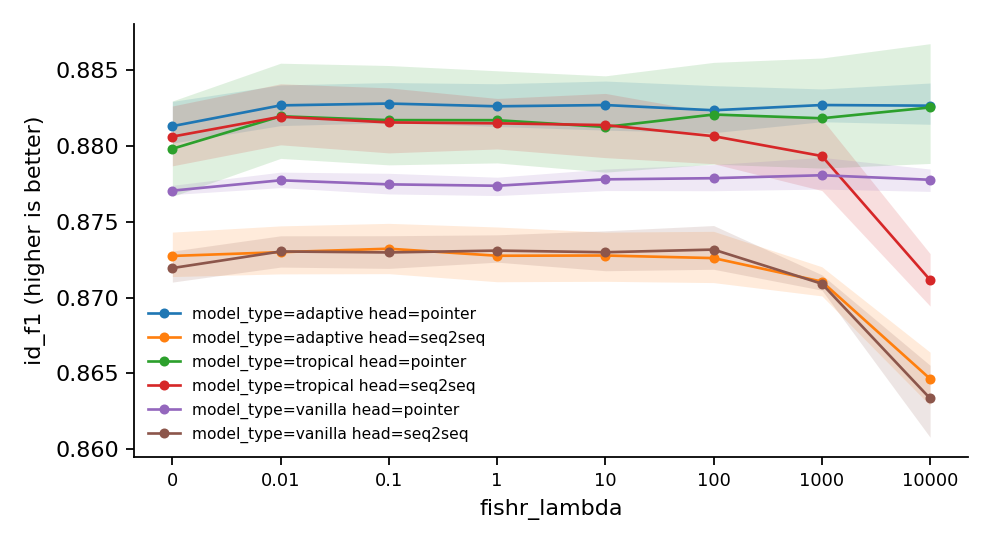
\includegraphics[width=\textwidth]{metric_id_f1.png}
\caption{\texttt{id\_f1} against \texttt{fishr\_lambda}: the mean over seeds with a 95\% bootstrap CI, one line per combination of the other factors.}
\label{fig:id_f1}
\end{figure}

{\small
\begin{longtable}{lllrlrrr}
\caption{\texttt{id\_f1} per cell: mean, 95\% bootstrap CI, SD, seeds, diverged runs.}\label{tab:summary-id_f1}\\
\toprule
\texttt{model\_type} & \texttt{head} & \texttt{fishr\_lambda} & mean & 95\% CI & SD & $n$ & div.\\
\midrule
\endhead
adaptive & pointer & 0 & 0.8813 & [0.88, 0.883] & 0.0018 & 5 & 0\\
adaptive & pointer & 0.01 & 0.8827 & [0.881, 0.884] & 0.00183 & 5 & 0\\
adaptive & pointer & 0.1 & 0.8828 & [0.882, 0.884] & 0.0018 & 5 & 0\\
adaptive & pointer & 1 & 0.8826 & [0.881, 0.884] & 0.00185 & 5 & 0\\
adaptive & pointer & 10 & 0.8827 & [0.881, 0.884] & 0.00214 & 5 & 0\\
adaptive & pointer & 100 & 0.8824 & [0.881, 0.884] & 0.00202 & 5 & 0\\
adaptive & pointer & 1000 & 0.8827 & [0.882, 0.884] & 0.00145 & 5 & 0\\
adaptive & pointer & 1e+04 & 0.8827 & [0.881, 0.884] & 0.00179 & 5 & 0\\
adaptive & seq2seq & 0 & 0.8728 & [0.871, 0.874] & 0.00198 & 5 & 0\\
adaptive & seq2seq & 0.01 & 0.873 & [0.872, 0.875] & 0.00206 & 5 & 0\\
adaptive & seq2seq & 0.1 & 0.8732 & [0.872, 0.875] & 0.00223 & 5 & 0\\
adaptive & seq2seq & 1 & 0.8728 & [0.871, 0.875] & 0.00239 & 5 & 0\\
adaptive & seq2seq & 10 & 0.8728 & [0.871, 0.874] & 0.0021 & 5 & 0\\
adaptive & seq2seq & 100 & 0.8726 & [0.871, 0.874] & 0.00224 & 5 & 0\\
adaptive & seq2seq & 1000 & 0.8711 & [0.87, 0.872] & 0.0012 & 5 & 0\\
adaptive & seq2seq & 1e+04 & 0.8646 & [0.863, 0.866] & 0.00229 & 5 & 0\\
tropical & pointer & 0 & 0.8798 & [0.877, 0.883] & 0.00433 & 5 & 0\\
tropical & pointer & 0.01 & 0.882 & [0.879, 0.885] & 0.00404 & 5 & 0\\
tropical & pointer & 0.1 & 0.8817 & [0.879, 0.885] & 0.00414 & 5 & 0\\
tropical & pointer & 1 & 0.8817 & [0.879, 0.885] & 0.00417 & 5 & 0\\
tropical & pointer & 10 & 0.8813 & [0.878, 0.885] & 0.00417 & 5 & 0\\
tropical & pointer & 100 & 0.8821 & [0.879, 0.886] & 0.00449 & 5 & 0\\
tropical & pointer & 1000 & 0.8818 & [0.879, 0.886] & 0.00464 & 5 & 0\\
tropical & pointer & 1e+04 & 0.8825 & [0.879, 0.887] & 0.00503 & 5 & 0\\
tropical & seq2seq & 0 & 0.8806 & [0.879, 0.883] & 0.00255 & 5 & 0\\
tropical & seq2seq & 0.01 & 0.8819 & [0.88, 0.884] & 0.00262 & 5 & 0\\
tropical & seq2seq & 0.1 & 0.8816 & [0.88, 0.884] & 0.00278 & 5 & 0\\
tropical & seq2seq & 1 & 0.8815 & [0.88, 0.883] & 0.0022 & 5 & 0\\
tropical & seq2seq & 10 & 0.8814 & [0.879, 0.883] & 0.0029 & 5 & 0\\
tropical & seq2seq & 100 & 0.8806 & [0.879, 0.882] & 0.00226 & 5 & 0\\
tropical & seq2seq & 1000 & 0.8793 & [0.877, 0.882] & 0.00316 & 5 & 0\\
tropical & seq2seq & 1e+04 & 0.8712 & [0.869, 0.873] & 0.00219 & 5 & 0\\
vanilla & pointer & 0 & 0.8771 & [0.877, 0.877] & $3.95\times10^{-4}$ & 5 & 0\\
vanilla & pointer & 0.01 & 0.8777 & [0.877, 0.878] & $6.14\times10^{-4}$ & 5 & 0\\
vanilla & pointer & 0.1 & 0.8775 & [0.877, 0.878] & $8.84\times10^{-4}$ & 5 & 0\\
vanilla & pointer & 1 & 0.8774 & [0.877, 0.878] & $7.44\times10^{-4}$ & 5 & 0\\
vanilla & pointer & 10 & 0.8778 & [0.877, 0.878] & $9.02\times10^{-4}$ & 5 & 0\\
vanilla & pointer & 100 & 0.8779 & [0.877, 0.879] & 0.00108 & 5 & 0\\
vanilla & pointer & 1000 & 0.8781 & [0.877, 0.879] & 0.00129 & 5 & 0\\
vanilla & pointer & 1e+04 & 0.8778 & [0.877, 0.878] & $9.84\times10^{-4}$ & 5 & 0\\
vanilla & seq2seq & 0 & 0.8719 & [0.871, 0.873] & 0.00135 & 5 & 0\\
vanilla & seq2seq & 0.01 & 0.873 & [0.872, 0.874] & 0.00132 & 5 & 0\\
vanilla & seq2seq & 0.1 & 0.873 & [0.872, 0.874] & 0.00142 & 5 & 0\\
vanilla & seq2seq & 1 & 0.8731 & [0.872, 0.874] & 0.00116 & 5 & 0\\
vanilla & seq2seq & 10 & 0.873 & [0.872, 0.874] & 0.00173 & 5 & 0\\
vanilla & seq2seq & 100 & 0.8732 & [0.872, 0.875] & 0.00193 & 5 & 0\\
vanilla & seq2seq & 1000 & 0.8709 & [0.87, 0.872] & $6.78\times10^{-4}$ & 5 & 0\\
vanilla & seq2seq & 1e+04 & 0.8634 & [0.861, 0.866] & 0.00323 & 5 & 0\\
\bottomrule
\end{longtable}
}

{\small
\begin{longtable}{lllrrrl}
\caption{\texttt{id\_f1}: each level of \texttt{fishr\_lambda} against its control (0), within each combination of the other factors. parametric: Dunnett vs control.}\label{tab:control-id_f1}\\
\toprule
\texttt{model\_type} & \texttt{head} & \texttt{fishr\_lambda} & difference & 95\% CI & $p$ & \\
\midrule
\endhead
adaptive & pointer & 0.01 & 0.001371 & [-0.00185, 0.00459] & 0.7458 & \\
adaptive & pointer & 0.1 & 0.001491 & [-0.00173, 0.00471] & 0.6742 & \\
adaptive & pointer & 1 & 0.00131 & [-0.00191, 0.00453] & 0.7804 & \\
adaptive & pointer & 10 & 0.001393 & [-0.00183, 0.00462] & 0.7328 & \\
adaptive & pointer & 100 & 0.001048 & [-0.00217, 0.00427] & 0.9051 & \\
adaptive & pointer & 1000 & 0.001394 & [-0.00183, 0.00462] & 0.7322 & \\
adaptive & pointer & 1e+04 & 0.001352 & [-0.00187, 0.00457] & 0.7569 & \\
adaptive & seq2seq & 0.01 & $2.477\times10^{-4}$ & [-0.00341, 0.0039] & 1.0000 & \\
adaptive & seq2seq & 0.1 & $4.762\times10^{-4}$ & [-0.00318, 0.00413] & 0.9994 & \\
adaptive & seq2seq & 1 & $1.276\times10^{-5}$ & [-0.00364, 0.00367] & 1.0000 & \\
adaptive & seq2seq & 10 & $2.783\times10^{-5}$ & [-0.00363, 0.00368] & 1.0000 & \\
adaptive & seq2seq & 100 & $-1.429\times10^{-4}$ & [-0.0038, 0.00351] & 1.0000 & \\
adaptive & seq2seq & 1000 & -0.001693 & [-0.00535, 0.00196] & 0.6739 & \\
adaptive & seq2seq & 1e+04 & -0.008105 & [-0.0118, -0.00445] & $<10^{-4}$ & *\\
tropical & pointer & 0.01 & 0.002142 & [-0.00552, 0.00981] & 0.9520 & \\
tropical & pointer & 0.1 & 0.001889 & [-0.00578, 0.00955] & 0.9743 & \\
tropical & pointer & 1 & 0.001886 & [-0.00578, 0.00955] & 0.9745 & \\
tropical & pointer & 10 & 0.001439 & [-0.00623, 0.0091] & 0.9942 & \\
tropical & pointer & 100 & 0.002259 & [-0.00541, 0.00992] & 0.9385 & \\
tropical & pointer & 1000 & 0.002012 & [-0.00565, 0.00968] & 0.9646 & \\
tropical & pointer & 1e+04 & 0.002726 & [-0.00494, 0.0104] & 0.8640 & \\
tropical & seq2seq & 0.01 & 0.001313 & [-0.00323, 0.00586] & 0.9439 & \\
tropical & seq2seq & 0.1 & $9.355\times10^{-4}$ & [-0.00361, 0.00548] & 0.9903 & \\
tropical & seq2seq & 1 & $8.775\times10^{-4}$ & [-0.00367, 0.00542] & 0.9932 & \\
tropical & seq2seq & 10 & $7.615\times10^{-4}$ & [-0.00378, 0.00531] & 0.9971 & \\
tropical & seq2seq & 100 & $2.869\times10^{-5}$ & [-0.00452, 0.00457] & 1.0000 & \\
tropical & seq2seq & 1000 & -0.00128 & [-0.00582, 0.00326] & 0.9502 & \\
tropical & seq2seq & 1e+04 & -0.009454 & [-0.014, -0.00491] & $<10^{-4}$ & *\\
vanilla & pointer & 0.01 & $6.832\times10^{-4}$ & [$-8.87\times10^{-4}$, 0.00225] & 0.7273 & \\
vanilla & pointer & 0.1 & $4.147\times10^{-4}$ & [-0.00116, 0.00198] & 0.9635 & \\
vanilla & pointer & 1 & $3.229\times10^{-4}$ & [-0.00125, 0.00189] & 0.9903 & \\
vanilla & pointer & 10 & $7.451\times10^{-4}$ & [$-8.25\times10^{-4}$, 0.00231] & 0.6509 & \\
vanilla & pointer & 100 & $8.221\times10^{-4}$ & [$-7.48\times10^{-4}$, 0.00239] & 0.5550 & \\
vanilla & pointer & 1000 & 0.001016 & [$-5.54\times10^{-4}$, 0.00259] & 0.3400 & \\
vanilla & pointer & 1e+04 & $7.178\times10^{-4}$ & [$-8.52\times10^{-4}$, 0.00229] & 0.6851 & \\
vanilla & seq2seq & 0.01 & 0.001096 & [-0.00197, 0.00416] & 0.8606 & \\
vanilla & seq2seq & 0.1 & 0.001031 & [-0.00203, 0.00409] & 0.8906 & \\
vanilla & seq2seq & 1 & 0.001153 & [-0.00191, 0.00422] & 0.8315 & \\
vanilla & seq2seq & 10 & 0.001044 & [-0.00202, 0.00411] & 0.8847 & \\
vanilla & seq2seq & 100 & 0.00122 & [-0.00184, 0.00428] & 0.7946 & \\
vanilla & seq2seq & 1000 & -0.001033 & [-0.0041, 0.00203] & 0.8896 & \\
vanilla & seq2seq & 1e+04 & -0.008597 & [-0.0117, -0.00554] & $<10^{-4}$ & *\\
\bottomrule
\end{longtable}
}

{\small
\begin{longtable}{llrrrrr}
\caption{\texttt{id\_f1} against log10 \texttt{fishr\_lambda}: parametric: OLS slope t-test, seed-bootstrap CI, with the Jonckheere--Terpstra ordered-trend $\tau$ and $p$.}\label{tab:trend-id_f1}\\
\toprule
\texttt{model\_type} & \texttt{head} & estimate & 95\% CI & $p$ & JT $\tau$ & JT $p$\\
\midrule
\endhead
adaptive & pointer & $-1.835\times10^{-5}$ & [$-7.11\times10^{-5}$, $2.83\times10^{-5}$] & 0.8997 & -0.0286 & 0.8416\\
adaptive & seq2seq & -0.001055 & [-0.00119, $-8.49\times10^{-4}$] & $<10^{-4}$ & -0.459 & 0.0008\\
tropical & pointer & $8.474\times10^{-5}$ & [$-8.85\times10^{-5}$, $2.58\times10^{-4}$] & 0.8066 & 0.00952 & 0.9486\\
tropical & seq2seq & -0.001342 & [-0.00148, -0.00121] & $<10^{-4}$ & -0.432 & 0.0012\\
vanilla & pointer & $6.449\times10^{-5}$ & [$-2.89\times10^{-5}$, $1.44\times10^{-4}$] & 0.3991 & 0.0971 & 0.4777\\
vanilla & seq2seq & -0.001184 & [-0.0016, $-8.05\times10^{-4}$] & $<10^{-4}$ & -0.482 & 0.0006\\
\bottomrule
\end{longtable}
}

{\small
\begin{longtable}{lrrrl}
\caption{\texttt{id\_f1}: paired contrasts by seed, Holm-corrected across the cells. parametric: paired t-test by seed, Holm.}\label{tab:paired-id_f1}\\
\toprule
contrast (within) & difference & 95\% CI & $p$ & \\
\midrule
\endhead
\stackcell{model\_type: tropical - vanilla\\\footnotesize head=pointer fishr\_lambda=0 } & 0.002761 & [-0.003, 0.00853] & 0.7368 & \\
\stackcell{model\_type: tropical - vanilla\\\footnotesize head=pointer fishr\_lambda=0.01 } & 0.00422 & [-0.00125, 0.00969] & 0.7368 & \\
\stackcell{model\_type: tropical - vanilla\\\footnotesize head=pointer fishr\_lambda=0.1 } & 0.004236 & [-0.00121, 0.00968] & 0.7368 & \\
\stackcell{model\_type: tropical - vanilla\\\footnotesize head=pointer fishr\_lambda=1 } & 0.004325 & [-0.00138, 0.01] & 0.7368 & \\
\stackcell{model\_type: tropical - vanilla\\\footnotesize head=pointer fishr\_lambda=10 } & 0.003456 & [-0.00214, 0.00905] & 0.7368 & \\
\stackcell{model\_type: tropical - vanilla\\\footnotesize head=pointer fishr\_lambda=100 } & 0.004198 & [-0.00197, 0.0104] & 0.7368 & \\
\stackcell{model\_type: tropical - vanilla\\\footnotesize head=pointer fishr\_lambda=1000 } & 0.003757 & [-0.00283, 0.0103] & 0.7368 & \\
\stackcell{model\_type: tropical - vanilla\\\footnotesize head=pointer fishr\_lambda=1e+04 } & 0.00477 & [-0.00124, 0.0108] & 0.7368 & \\
\stackcell{model\_type: tropical - vanilla\\\footnotesize head=seq2seq fishr\_lambda=0 } & 0.008669 & [0.00542, 0.0119] & 0.0284 & *\\
\stackcell{model\_type: tropical - vanilla\\\footnotesize head=seq2seq fishr\_lambda=0.01 } & 0.008886 & [0.00468, 0.0131] & 0.0508 & \\
\stackcell{model\_type: tropical - vanilla\\\footnotesize head=seq2seq fishr\_lambda=0.1 } & 0.008574 & [0.00392, 0.0132] & 0.0763 & \\
\stackcell{model\_type: tropical - vanilla\\\footnotesize head=seq2seq fishr\_lambda=1 } & 0.008394 & [0.00523, 0.0116] & 0.0284 & *\\
\stackcell{model\_type: tropical - vanilla\\\footnotesize head=seq2seq fishr\_lambda=10 } & 0.008386 & [0.00356, 0.0132] & 0.0770 & \\
\stackcell{model\_type: tropical - vanilla\\\footnotesize head=seq2seq fishr\_lambda=100 } & 0.007478 & [0.00329, 0.0117] & 0.0770 & \\
\stackcell{model\_type: tropical - vanilla\\\footnotesize head=seq2seq fishr\_lambda=1000 } & 0.008423 & [0.00493, 0.0119] & 0.0336 & *\\
\stackcell{model\_type: tropical - vanilla\\\footnotesize head=seq2seq fishr\_lambda=1e+04 } & 0.007813 & [0.00483, 0.0108] & 0.0284 & *\\
\stackcell{model\_type: adaptive - vanilla\\\footnotesize head=pointer fishr\_lambda=0 } & 0.004253 & [0.00247, 0.00604] & 0.0298 & *\\
\stackcell{model\_type: adaptive - vanilla\\\footnotesize head=pointer fishr\_lambda=0.01 } & 0.004941 & [0.00282, 0.00706] & 0.0298 & *\\
\stackcell{model\_type: adaptive - vanilla\\\footnotesize head=pointer fishr\_lambda=0.1 } & 0.00533 & [0.00354, 0.00712] & 0.0165 & *\\
\stackcell{model\_type: adaptive - vanilla\\\footnotesize head=pointer fishr\_lambda=1 } & 0.00524 & [0.00329, 0.00719] & 0.0222 & *\\
\stackcell{model\_type: adaptive - vanilla\\\footnotesize head=pointer fishr\_lambda=10 } & 0.004901 & [0.00282, 0.00699] & 0.0298 & *\\
\stackcell{model\_type: adaptive - vanilla\\\footnotesize head=pointer fishr\_lambda=100 } & 0.004479 & [0.0028, 0.00616] & 0.0222 & *\\
\stackcell{model\_type: adaptive - vanilla\\\footnotesize head=pointer fishr\_lambda=1000 } & 0.004631 & [0.00311, 0.00615] & 0.0161 & *\\
\stackcell{model\_type: adaptive - vanilla\\\footnotesize head=pointer fishr\_lambda=1e+04 } & 0.004887 & [0.00332, 0.00645] & 0.0156 & *\\
\stackcell{model\_type: adaptive - vanilla\\\footnotesize head=seq2seq fishr\_lambda=0 } & $8.006\times10^{-4}$ & [-0.00109, 0.0027] & 1.0000 & \\
\stackcell{model\_type: adaptive - vanilla\\\footnotesize head=seq2seq fishr\_lambda=0.01 } & $-4.780\times10^{-5}$ & [-0.00287, 0.00278] & 1.0000 & \\
\stackcell{model\_type: adaptive - vanilla\\\footnotesize head=seq2seq fishr\_lambda=0.1 } & $2.458\times10^{-4}$ & [-0.00262, 0.00311] & 1.0000 & \\
\stackcell{model\_type: adaptive - vanilla\\\footnotesize head=seq2seq fishr\_lambda=1 } & $-3.399\times10^{-4}$ & [-0.00328, 0.0026] & 1.0000 & \\
\stackcell{model\_type: adaptive - vanilla\\\footnotesize head=seq2seq fishr\_lambda=10 } & $-2.161\times10^{-4}$ & [-0.0033, 0.00287] & 1.0000 & \\
\stackcell{model\_type: adaptive - vanilla\\\footnotesize head=seq2seq fishr\_lambda=100 } & $-5.623\times10^{-4}$ & [-0.00388, 0.00275] & 1.0000 & \\
\stackcell{model\_type: adaptive - vanilla\\\footnotesize head=seq2seq fishr\_lambda=1000 } & $1.414\times10^{-4}$ & [$-7.11\times10^{-4}$, $9.93\times10^{-4}$] & 1.0000 & \\
\stackcell{model\_type: adaptive - vanilla\\\footnotesize head=seq2seq fishr\_lambda=1e+04 } & 0.001293 & [$-4.73\times10^{-4}$, 0.00306] & 0.8954 & \\
\stackcell{head: pointer - seq2seq\\\footnotesize model\_type=adaptive fishr\_lambda=0 } & 0.008559 & [0.0078, 0.00932] & 0.0001 & *\\
\stackcell{head: pointer - seq2seq\\\footnotesize model\_type=adaptive fishr\_lambda=0.01 } & 0.009682 & [0.00779, 0.0116] & 0.0024 & *\\
\stackcell{head: pointer - seq2seq\\\footnotesize model\_type=adaptive fishr\_lambda=0.1 } & 0.009574 & [0.00754, 0.0116] & 0.0029 & *\\
\stackcell{head: pointer - seq2seq\\\footnotesize model\_type=adaptive fishr\_lambda=1 } & 0.009856 & [0.00812, 0.0116] & 0.0019 & *\\
\stackcell{head: pointer - seq2seq\\\footnotesize model\_type=adaptive fishr\_lambda=10 } & 0.009924 & [0.00812, 0.0117] & 0.0019 & *\\
\stackcell{head: pointer - seq2seq\\\footnotesize model\_type=adaptive fishr\_lambda=100 } & 0.00975 & [0.00801, 0.0115] & 0.0019 & *\\
\stackcell{head: pointer - seq2seq\\\footnotesize model\_type=adaptive fishr\_lambda=1000 } & 0.01165 & [0.0109, 0.0124] & $<10^{-4}$ & *\\
\stackcell{head: pointer - seq2seq\\\footnotesize model\_type=adaptive fishr\_lambda=1e+04 } & 0.01802 & [0.0164, 0.0196] & 0.0001 & *\\
\stackcell{head: pointer - seq2seq\\\footnotesize model\_type=tropical fishr\_lambda=0 } & $-8.019\times10^{-4}$ & [-0.00707, 0.00547] & 1.0000 & \\
\stackcell{head: pointer - seq2seq\\\footnotesize model\_type=tropical fishr\_lambda=0.01 } & $2.710\times10^{-5}$ & [-0.00619, 0.00624] & 1.0000 & \\
\stackcell{head: pointer - seq2seq\\\footnotesize model\_type=tropical fishr\_lambda=0.1 } & $1.518\times10^{-4}$ & [-0.00529, 0.00559] & 1.0000 & \\
\stackcell{head: pointer - seq2seq\\\footnotesize model\_type=tropical fishr\_lambda=1 } & $2.067\times10^{-4}$ & [-0.00573, 0.00614] & 1.0000 & \\
\stackcell{head: pointer - seq2seq\\\footnotesize model\_type=tropical fishr\_lambda=10 } & $-1.240\times10^{-4}$ & [-0.00552, 0.00527] & 1.0000 & \\
\stackcell{head: pointer - seq2seq\\\footnotesize model\_type=tropical fishr\_lambda=100 } & 0.001429 & [-0.00448, 0.00734] & 1.0000 & \\
\stackcell{head: pointer - seq2seq\\\footnotesize model\_type=tropical fishr\_lambda=1000 } & 0.00249 & [-0.0046, 0.00958] & 1.0000 & \\
\stackcell{head: pointer - seq2seq\\\footnotesize model\_type=tropical fishr\_lambda=1e+04 } & 0.01138 & [0.00514, 0.0176] & 0.0607 & \\
\stackcell{head: pointer - seq2seq\\\footnotesize model\_type=vanilla fishr\_lambda=0 } & 0.005106 & [0.00357, 0.00664] & 0.0107 & *\\
\stackcell{head: pointer - seq2seq\\\footnotesize model\_type=vanilla fishr\_lambda=0.01 } & 0.004693 & [0.00317, 0.00622] & 0.0134 & *\\
\stackcell{head: pointer - seq2seq\\\footnotesize model\_type=vanilla fishr\_lambda=0.1 } & 0.00449 & [0.00258, 0.0064] & 0.0312 & *\\
\stackcell{head: pointer - seq2seq\\\footnotesize model\_type=vanilla fishr\_lambda=1 } & 0.004276 & [0.00272, 0.00583] & 0.0189 & *\\
\stackcell{head: pointer - seq2seq\\\footnotesize model\_type=vanilla fishr\_lambda=10 } & 0.004807 & [0.00253, 0.00709] & 0.0424 & *\\
\stackcell{head: pointer - seq2seq\\\footnotesize model\_type=vanilla fishr\_lambda=100 } & 0.004708 & [0.00217, 0.00725] & 0.0607 & \\
\stackcell{head: pointer - seq2seq\\\footnotesize model\_type=vanilla fishr\_lambda=1000 } & 0.007156 & [0.00617, 0.00814] & 0.0007 & *\\
\stackcell{head: pointer - seq2seq\\\footnotesize model\_type=vanilla fishr\_lambda=1e+04 } & 0.01442 & [0.0116, 0.0172] & 0.0024 & *\\
\bottomrule
\end{longtable}
}

\subsection{\texttt{id\_exact}}
\begin{figure}[tbp]
\centering
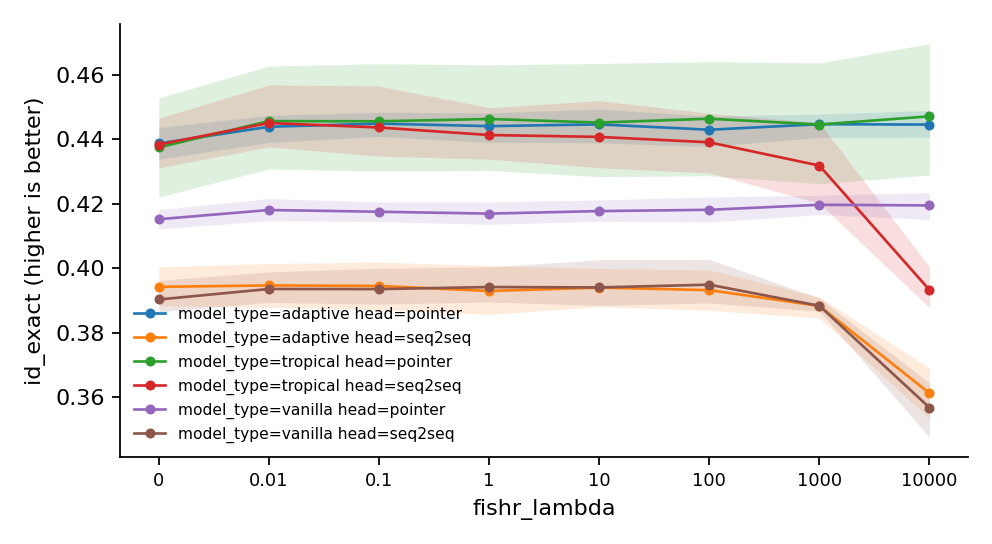
\includegraphics[width=\textwidth]{metric_id_exact.png}
\caption{\texttt{id\_exact} against \texttt{fishr\_lambda}: the mean over seeds with a 95\% bootstrap CI, one line per combination of the other factors.}
\label{fig:id_exact}
\end{figure}

{\small
\begin{longtable}{lllrlrrr}
\caption{\texttt{id\_exact} per cell: mean, 95\% bootstrap CI, SD, seeds, diverged runs.}\label{tab:summary-id_exact}\\
\toprule
\texttt{model\_type} & \texttt{head} & \texttt{fishr\_lambda} & mean & 95\% CI & SD & $n$ & div.\\
\midrule
\endhead
adaptive & pointer & 0 & 0.4388 & [0.434, 0.444] & 0.00652 & 5 & 0\\
adaptive & pointer & 0.01 & 0.4439 & [0.439, 0.447] & 0.00575 & 5 & 0\\
adaptive & pointer & 0.1 & 0.4449 & [0.441, 0.448] & 0.00504 & 5 & 0\\
adaptive & pointer & 1 & 0.4441 & [0.439, 0.448] & 0.00552 & 5 & 0\\
adaptive & pointer & 10 & 0.4447 & [0.439, 0.449] & 0.00694 & 5 & 0\\
adaptive & pointer & 100 & 0.443 & [0.438, 0.447] & 0.00597 & 5 & 0\\
adaptive & pointer & 1000 & 0.4447 & [0.441, 0.448] & 0.00471 & 5 & 0\\
adaptive & pointer & 1e+04 & 0.4446 & [0.441, 0.449] & 0.0055 & 5 & 0\\
adaptive & seq2seq & 0 & 0.3943 & [0.388, 0.4] & 0.00811 & 5 & 0\\
adaptive & seq2seq & 0.01 & 0.3947 & [0.388, 0.402] & 0.00879 & 5 & 0\\
adaptive & seq2seq & 0.1 & 0.3946 & [0.387, 0.402] & 0.00981 & 5 & 0\\
adaptive & seq2seq & 1 & 0.393 & [0.386, 0.401] & 0.00965 & 5 & 0\\
adaptive & seq2seq & 10 & 0.394 & [0.388, 0.4] & 0.00788 & 5 & 0\\
adaptive & seq2seq & 100 & 0.3933 & [0.387, 0.4] & 0.00806 & 5 & 0\\
adaptive & seq2seq & 1000 & 0.3884 & [0.385, 0.391] & 0.00416 & 5 & 0\\
adaptive & seq2seq & 1e+04 & 0.3613 & [0.353, 0.369] & 0.0101 & 5 & 0\\
tropical & pointer & 0 & 0.4375 & [0.422, 0.453] & 0.0209 & 5 & 0\\
tropical & pointer & 0.01 & 0.4457 & [0.431, 0.463] & 0.0212 & 5 & 0\\
tropical & pointer & 0.1 & 0.4456 & [0.43, 0.463] & 0.0211 & 5 & 0\\
tropical & pointer & 1 & 0.4464 & [0.43, 0.463] & 0.0226 & 5 & 0\\
tropical & pointer & 10 & 0.4452 & [0.428, 0.464] & 0.0223 & 5 & 0\\
tropical & pointer & 100 & 0.4464 & [0.429, 0.464] & 0.0243 & 5 & 0\\
tropical & pointer & 1000 & 0.4446 & [0.426, 0.464] & 0.025 & 5 & 0\\
tropical & pointer & 1e+04 & 0.4472 & [0.429, 0.47] & 0.0256 & 5 & 0\\
tropical & seq2seq & 0 & 0.4384 & [0.431, 0.447] & 0.0104 & 5 & 0\\
tropical & seq2seq & 0.01 & 0.4451 & [0.438, 0.457] & 0.013 & 5 & 0\\
tropical & seq2seq & 0.1 & 0.4437 & [0.435, 0.457] & 0.0141 & 5 & 0\\
tropical & seq2seq & 1 & 0.4414 & [0.434, 0.45] & 0.0101 & 5 & 0\\
tropical & seq2seq & 10 & 0.4408 & [0.431, 0.452] & 0.0132 & 5 & 0\\
tropical & seq2seq & 100 & 0.4391 & [0.43, 0.448] & 0.0115 & 5 & 0\\
tropical & seq2seq & 1000 & 0.4319 & [0.42, 0.445] & 0.016 & 5 & 0\\
tropical & seq2seq & 1e+04 & 0.3933 & [0.388, 0.401] & 0.00817 & 5 & 0\\
vanilla & pointer & 0 & 0.4153 & [0.412, 0.418] & 0.00408 & 5 & 0\\
vanilla & pointer & 0.01 & 0.4181 & [0.415, 0.422] & 0.00441 & 5 & 0\\
vanilla & pointer & 0.1 & 0.4176 & [0.415, 0.421] & 0.00408 & 5 & 0\\
vanilla & pointer & 1 & 0.417 & [0.414, 0.421] & 0.00469 & 5 & 0\\
vanilla & pointer & 10 & 0.4178 & [0.415, 0.421] & 0.00419 & 5 & 0\\
vanilla & pointer & 100 & 0.4182 & [0.414, 0.422] & 0.0051 & 5 & 0\\
vanilla & pointer & 1000 & 0.4197 & [0.417, 0.423] & 0.0038 & 5 & 0\\
vanilla & pointer & 1e+04 & 0.4195 & [0.415, 0.424] & 0.00559 & 5 & 0\\
vanilla & seq2seq & 0 & 0.3904 & [0.387, 0.396] & 0.00657 & 5 & 0\\
vanilla & seq2seq & 0.01 & 0.3936 & [0.389, 0.399] & 0.00605 & 5 & 0\\
vanilla & seq2seq & 0.1 & 0.3936 & [0.389, 0.4] & 0.0072 & 5 & 0\\
vanilla & seq2seq & 1 & 0.3942 & [0.39, 0.4] & 0.00708 & 5 & 0\\
vanilla & seq2seq & 10 & 0.3941 & [0.388, 0.403] & 0.00958 & 5 & 0\\
vanilla & seq2seq & 100 & 0.395 & [0.389, 0.403] & 0.00883 & 5 & 0\\
vanilla & seq2seq & 1000 & 0.3884 & [0.387, 0.391] & 0.00273 & 5 & 0\\
vanilla & seq2seq & 1e+04 & 0.3568 & [0.348, 0.364] & 0.011 & 5 & 0\\
\bottomrule
\end{longtable}
}

{\small
\begin{longtable}{lllrrrl}
\caption{\texttt{id\_exact}: each level of \texttt{fishr\_lambda} against its control (0), within each combination of the other factors. parametric: Dunnett vs control.}\label{tab:control-id_exact}\\
\toprule
\texttt{model\_type} & \texttt{head} & \texttt{fishr\_lambda} & difference & 95\% CI & $p$ & \\
\midrule
\endhead
adaptive & pointer & 0.01 & 0.00518 & [-0.00492, 0.0153] & 0.5764 & \\
adaptive & pointer & 0.1 & 0.00616 & [-0.00394, 0.0163] & 0.3995 & \\
adaptive & pointer & 1 & 0.00538 & [-0.00472, 0.0155] & 0.5382 & \\
adaptive & pointer & 10 & 0.00592 & [-0.00418, 0.016] & 0.4400 & \\
adaptive & pointer & 100 & 0.00426 & [-0.00584, 0.0144] & 0.7527 & \\
adaptive & pointer & 1000 & 0.00598 & [-0.00412, 0.0161] & 0.4297 & \\
adaptive & pointer & 1e+04 & 0.00586 & [-0.00424, 0.016] & 0.4505 & \\
adaptive & seq2seq & 0.01 & $4.400\times10^{-4}$ & [-0.0144, 0.0153] & 1.0000 & \\
adaptive & seq2seq & 0.1 & $2.800\times10^{-4}$ & [-0.0146, 0.0151] & 1.0000 & \\
adaptive & seq2seq & 1 & -0.00128 & [-0.0161, 0.0136] & 1.0000 & \\
adaptive & seq2seq & 10 & $-2.400\times10^{-4}$ & [-0.0151, 0.0146] & 1.0000 & \\
adaptive & seq2seq & 100 & -0.00102 & [-0.0159, 0.0138] & 1.0000 & \\
adaptive & seq2seq & 1000 & -0.00592 & [-0.0208, 0.00894] & 0.7950 & \\
adaptive & seq2seq & 1e+04 & -0.033 & [-0.0479, -0.0181] & $<10^{-4}$ & *\\
tropical & pointer & 0.01 & 0.00816 & [-0.0319, 0.0482] & 0.9908 & \\
tropical & pointer & 0.1 & 0.0081 & [-0.032, 0.0482] & 0.9912 & \\
tropical & pointer & 1 & 0.00882 & [-0.0312, 0.0489] & 0.9859 & \\
tropical & pointer & 10 & 0.0077 & [-0.0324, 0.0478] & 0.9934 & \\
tropical & pointer & 100 & 0.0089 & [-0.0312, 0.049] & 0.9852 & \\
tropical & pointer & 1000 & 0.0071 & [-0.033, 0.0472] & 0.9959 & \\
tropical & pointer & 1e+04 & 0.00964 & [-0.0304, 0.0497] & 0.9773 & \\
tropical & seq2seq & 0.01 & 0.0067 & [-0.0148, 0.0282] & 0.9207 & \\
tropical & seq2seq & 0.1 & 0.0053 & [-0.0162, 0.0268] & 0.9741 & \\
tropical & seq2seq & 1 & 0.00296 & [-0.0185, 0.0244] & 0.9991 & \\
tropical & seq2seq & 10 & 0.00238 & [-0.0191, 0.0239] & 0.9998 & \\
tropical & seq2seq & 100 & $7.000\times10^{-4}$ & [-0.0208, 0.0222] & 1.0000 & \\
tropical & seq2seq & 1000 & -0.00652 & [-0.028, 0.015] & 0.9297 & \\
tropical & seq2seq & 1e+04 & -0.0451 & [-0.0666, -0.0236] & $<10^{-4}$ & *\\
vanilla & pointer & 0.01 & 0.00286 & [-0.00505, 0.0108] & 0.8550 & \\
vanilla & pointer & 0.1 & 0.00232 & [-0.00559, 0.0102] & 0.9398 & \\
vanilla & pointer & 1 & 0.00174 & [-0.00617, 0.00965] & 0.9859 & \\
vanilla & pointer & 10 & 0.00252 & [-0.00539, 0.0104] & 0.9131 & \\
vanilla & pointer & 100 & 0.00292 & [-0.00499, 0.0108] & 0.8432 & \\
vanilla & pointer & 1000 & 0.00448 & [-0.00343, 0.0124] & 0.4747 & \\
vanilla & pointer & 1e+04 & 0.00428 & [-0.00363, 0.0122] & 0.5217 & \\
vanilla & seq2seq & 0.01 & 0.00326 & [-0.0103, 0.0168] & 0.9772 & \\
vanilla & seq2seq & 0.1 & 0.00322 & [-0.0103, 0.0168] & 0.9787 & \\
vanilla & seq2seq & 1 & 0.00386 & [-0.00968, 0.0174] & 0.9474 & \\
vanilla & seq2seq & 10 & 0.00374 & [-0.0098, 0.0173] & 0.9547 & \\
vanilla & seq2seq & 100 & 0.0046 & [-0.00894, 0.0181] & 0.8866 & \\
vanilla & seq2seq & 1000 & -0.00196 & [-0.0155, 0.0116] & 0.9988 & \\
vanilla & seq2seq & 1e+04 & -0.03354 & [-0.0471, -0.02] & $<10^{-4}$ & *\\
\bottomrule
\end{longtable}
}

{\small
\begin{longtable}{llrrrrr}
\caption{\texttt{id\_exact} against log10 \texttt{fishr\_lambda}: parametric: OLS slope t-test, seed-bootstrap CI, with the Jonckheere--Terpstra ordered-trend $\tau$ and $p$.}\label{tab:trend-id_exact}\\
\toprule
\texttt{model\_type} & \texttt{head} & estimate & 95\% CI & $p$ & JT $\tau$ & JT $p$\\
\midrule
\endhead
adaptive & pointer & $2.000\times10^{-5}$ & [$-1.95\times10^{-4}$, $2.35\times10^{-4}$] & 0.9644 & -0.0171 & 0.9072\\
adaptive & seq2seq & -0.004016 & [-0.00464, -0.00338] & 0.0002 & -0.385 & 0.0020\\
tropical & pointer & $9.000\times10^{-5}$ & [$-7.22\times10^{-4}$, $9.02\times10^{-4}$] & 0.9606 & 0.0133 & 0.9354\\
tropical & seq2seq & -0.006475 & [-0.00712, -0.00583] & $<10^{-4}$ & -0.436 & 0.0008\\
vanilla & pointer & $3.486\times10^{-4}$ & [$-4.07\times10^{-5}$, $7.23\times10^{-4}$] & 0.3415 & 0.105 & 0.4429\\
vanilla & seq2seq & -0.004286 & [-0.00571, -0.00291] & 0.0002 & -0.444 & 0.0010\\
\bottomrule
\end{longtable}
}

{\small
\begin{longtable}{lrrrl}
\caption{\texttt{id\_exact}: paired contrasts by seed, Holm-corrected across the cells. parametric: paired t-test by seed, Holm.}\label{tab:paired-id_exact}\\
\toprule
contrast (within) & difference & 95\% CI & $p$ & \\
\midrule
\endhead
\stackcell{model\_type: tropical - vanilla\\\footnotesize head=pointer fishr\_lambda=0 } & 0.02228 & [-0.00221, 0.0468] & 0.2778 & \\
\stackcell{model\_type: tropical - vanilla\\\footnotesize head=pointer fishr\_lambda=0.01 } & 0.02758 & [0.00322, 0.0519] & 0.2778 & \\
\stackcell{model\_type: tropical - vanilla\\\footnotesize head=pointer fishr\_lambda=0.1 } & 0.02806 & [0.0029, 0.0532] & 0.2778 & \\
\stackcell{model\_type: tropical - vanilla\\\footnotesize head=pointer fishr\_lambda=1 } & 0.02936 & [0.00305, 0.0557] & 0.2778 & \\
\stackcell{model\_type: tropical - vanilla\\\footnotesize head=pointer fishr\_lambda=10 } & 0.02746 & [$8.05\times10^{-4}$, 0.0541] & 0.2778 & \\
\stackcell{model\_type: tropical - vanilla\\\footnotesize head=pointer fishr\_lambda=100 } & 0.02826 & [$-1.26\times10^{-4}$, 0.0566] & 0.2778 & \\
\stackcell{model\_type: tropical - vanilla\\\footnotesize head=pointer fishr\_lambda=1000 } & 0.0249 & [-0.00505, 0.0548] & 0.2778 & \\
\stackcell{model\_type: tropical - vanilla\\\footnotesize head=pointer fishr\_lambda=1e+04 } & 0.02764 & [$9.13\times10^{-4}$, 0.0544] & 0.2778 & \\
\stackcell{model\_type: tropical - vanilla\\\footnotesize head=seq2seq fishr\_lambda=0 } & 0.04806 & [0.0325, 0.0637] & 0.0164 & *\\
\stackcell{model\_type: tropical - vanilla\\\footnotesize head=seq2seq fishr\_lambda=0.01 } & 0.0515 & [0.0314, 0.0716] & 0.0267 & *\\
\stackcell{model\_type: tropical - vanilla\\\footnotesize head=seq2seq fishr\_lambda=0.1 } & 0.05014 & [0.0275, 0.0727] & 0.0423 & *\\
\stackcell{model\_type: tropical - vanilla\\\footnotesize head=seq2seq fishr\_lambda=1 } & 0.04716 & [0.03, 0.0643] & 0.0228 & *\\
\stackcell{model\_type: tropical - vanilla\\\footnotesize head=seq2seq fishr\_lambda=10 } & 0.0467 & [0.0249, 0.0685] & 0.0423 & *\\
\stackcell{model\_type: tropical - vanilla\\\footnotesize head=seq2seq fishr\_lambda=100 } & 0.04416 & [0.0237, 0.0646] & 0.0423 & *\\
\stackcell{model\_type: tropical - vanilla\\\footnotesize head=seq2seq fishr\_lambda=1000 } & 0.0435 & [0.0237, 0.0633] & 0.0423 & *\\
\stackcell{model\_type: tropical - vanilla\\\footnotesize head=seq2seq fishr\_lambda=1e+04 } & 0.0365 & [0.0234, 0.0496] & 0.0228 & *\\
\stackcell{model\_type: adaptive - vanilla\\\footnotesize head=pointer fishr\_lambda=0 } & 0.0235 & [0.0133, 0.0337] & 0.0273 & *\\
\stackcell{model\_type: adaptive - vanilla\\\footnotesize head=pointer fishr\_lambda=0.01 } & 0.02582 & [0.0166, 0.0351] & 0.0194 & *\\
\stackcell{model\_type: adaptive - vanilla\\\footnotesize head=pointer fishr\_lambda=0.1 } & 0.02734 & [0.0188, 0.0359] & 0.0135 & *\\
\stackcell{model\_type: adaptive - vanilla\\\footnotesize head=pointer fishr\_lambda=1 } & 0.02714 & [0.0173, 0.037] & 0.0194 & *\\
\stackcell{model\_type: adaptive - vanilla\\\footnotesize head=pointer fishr\_lambda=10 } & 0.0269 & [0.0172, 0.0366] & 0.0194 & *\\
\stackcell{model\_type: adaptive - vanilla\\\footnotesize head=pointer fishr\_lambda=100 } & 0.02484 & [0.017, 0.0326] & 0.0135 & *\\
\stackcell{model\_type: adaptive - vanilla\\\footnotesize head=pointer fishr\_lambda=1000 } & 0.025 & [0.0179, 0.0321] & 0.0099 & *\\
\stackcell{model\_type: adaptive - vanilla\\\footnotesize head=pointer fishr\_lambda=1e+04 } & 0.02508 & [0.0154, 0.0347] & 0.0197 & *\\
\stackcell{model\_type: adaptive - vanilla\\\footnotesize head=seq2seq fishr\_lambda=0 } & 0.00392 & [-0.00756, 0.0154] & 1.0000 & \\
\stackcell{model\_type: adaptive - vanilla\\\footnotesize head=seq2seq fishr\_lambda=0.01 } & 0.0011 & [-0.0112, 0.0134] & 1.0000 & \\
\stackcell{model\_type: adaptive - vanilla\\\footnotesize head=seq2seq fishr\_lambda=0.1 } & $9.800\times10^{-4}$ & [-0.0125, 0.0144] & 1.0000 & \\
\stackcell{model\_type: adaptive - vanilla\\\footnotesize head=seq2seq fishr\_lambda=1 } & -0.00122 & [-0.0162, 0.0137] & 1.0000 & \\
\stackcell{model\_type: adaptive - vanilla\\\footnotesize head=seq2seq fishr\_lambda=10 } & $-6.000\times10^{-5}$ & [-0.0133, 0.0132] & 1.0000 & \\
\stackcell{model\_type: adaptive - vanilla\\\footnotesize head=seq2seq fishr\_lambda=100 } & -0.0017 & [-0.0142, 0.0108] & 1.0000 & \\
\stackcell{model\_type: adaptive - vanilla\\\footnotesize head=seq2seq fishr\_lambda=1000 } & $-4.000\times10^{-5}$ & [-0.00464, 0.00456] & 1.0000 & \\
\stackcell{model\_type: adaptive - vanilla\\\footnotesize head=seq2seq fishr\_lambda=1e+04 } & 0.00446 & [-0.0055, 0.0144] & 1.0000 & \\
\stackcell{head: pointer - seq2seq\\\footnotesize model\_type=adaptive fishr\_lambda=0 } & 0.04448 & [0.0398, 0.0491] & 0.0003 & *\\
\stackcell{head: pointer - seq2seq\\\footnotesize model\_type=adaptive fishr\_lambda=0.01 } & 0.04922 & [0.0403, 0.0581] & 0.0018 & *\\
\stackcell{head: pointer - seq2seq\\\footnotesize model\_type=adaptive fishr\_lambda=0.1 } & 0.05036 & [0.0411, 0.0596] & 0.0018 & *\\
\stackcell{head: pointer - seq2seq\\\footnotesize model\_type=adaptive fishr\_lambda=1 } & 0.05114 & [0.0448, 0.0575] & 0.0005 & *\\
\stackcell{head: pointer - seq2seq\\\footnotesize model\_type=adaptive fishr\_lambda=10 } & 0.05064 & [0.0429, 0.0584] & 0.0010 & *\\
\stackcell{head: pointer - seq2seq\\\footnotesize model\_type=adaptive fishr\_lambda=100 } & 0.04976 & [0.0438, 0.0557] & 0.0004 & *\\
\stackcell{head: pointer - seq2seq\\\footnotesize model\_type=adaptive fishr\_lambda=1000 } & 0.05638 & [0.0523, 0.0605] & $<10^{-4}$ & *\\
\stackcell{head: pointer - seq2seq\\\footnotesize model\_type=adaptive fishr\_lambda=1e+04 } & 0.08334 & [0.0759, 0.0908] & 0.0001 & *\\
\stackcell{head: pointer - seq2seq\\\footnotesize model\_type=tropical fishr\_lambda=0 } & $-8.800\times10^{-4}$ & [-0.0284, 0.0267] & 1.0000 & \\
\stackcell{head: pointer - seq2seq\\\footnotesize model\_type=tropical fishr\_lambda=0.01 } & $5.800\times10^{-4}$ & [-0.0279, 0.0291] & 1.0000 & \\
\stackcell{head: pointer - seq2seq\\\footnotesize model\_type=tropical fishr\_lambda=0.1 } & 0.00192 & [-0.0245, 0.0283] & 1.0000 & \\
\stackcell{head: pointer - seq2seq\\\footnotesize model\_type=tropical fishr\_lambda=1 } & 0.00498 & [-0.0198, 0.0298] & 1.0000 & \\
\stackcell{head: pointer - seq2seq\\\footnotesize model\_type=tropical fishr\_lambda=10 } & 0.00444 & [-0.0227, 0.0316] & 1.0000 & \\
\stackcell{head: pointer - seq2seq\\\footnotesize model\_type=tropical fishr\_lambda=100 } & 0.00732 & [-0.0226, 0.0372] & 1.0000 & \\
\stackcell{head: pointer - seq2seq\\\footnotesize model\_type=tropical fishr\_lambda=1000 } & 0.01274 & [-0.0254, 0.0509] & 1.0000 & \\
\stackcell{head: pointer - seq2seq\\\footnotesize model\_type=tropical fishr\_lambda=1e+04 } & 0.05386 & [0.0244, 0.0833] & 0.0570 & \\
\stackcell{head: pointer - seq2seq\\\footnotesize model\_type=vanilla fishr\_lambda=0 } & 0.0249 & [0.0195, 0.0303] & 0.0030 & *\\
\stackcell{head: pointer - seq2seq\\\footnotesize model\_type=vanilla fishr\_lambda=0.01 } & 0.0245 & [0.0184, 0.0306] & 0.0045 & *\\
\stackcell{head: pointer - seq2seq\\\footnotesize model\_type=vanilla fishr\_lambda=0.1 } & 0.024 & [0.0165, 0.0315] & 0.0097 & *\\
\stackcell{head: pointer - seq2seq\\\footnotesize model\_type=vanilla fishr\_lambda=1 } & 0.02278 & [0.0176, 0.028] & 0.0034 & *\\
\stackcell{head: pointer - seq2seq\\\footnotesize model\_type=vanilla fishr\_lambda=10 } & 0.02368 & [0.0144, 0.033] & 0.0209 & *\\
\stackcell{head: pointer - seq2seq\\\footnotesize model\_type=vanilla fishr\_lambda=100 } & 0.02322 & [0.0134, 0.0331] & 0.0252 & *\\
\stackcell{head: pointer - seq2seq\\\footnotesize model\_type=vanilla fishr\_lambda=1000 } & 0.03134 & [0.0266, 0.0361] & 0.0010 & *\\
\stackcell{head: pointer - seq2seq\\\footnotesize model\_type=vanilla fishr\_lambda=1e+04 } & 0.06272 & [0.0512, 0.0742] & 0.0018 & *\\
\bottomrule
\end{longtable}
}


\section{Curves}
\begin{figure}[tbp]
\centering
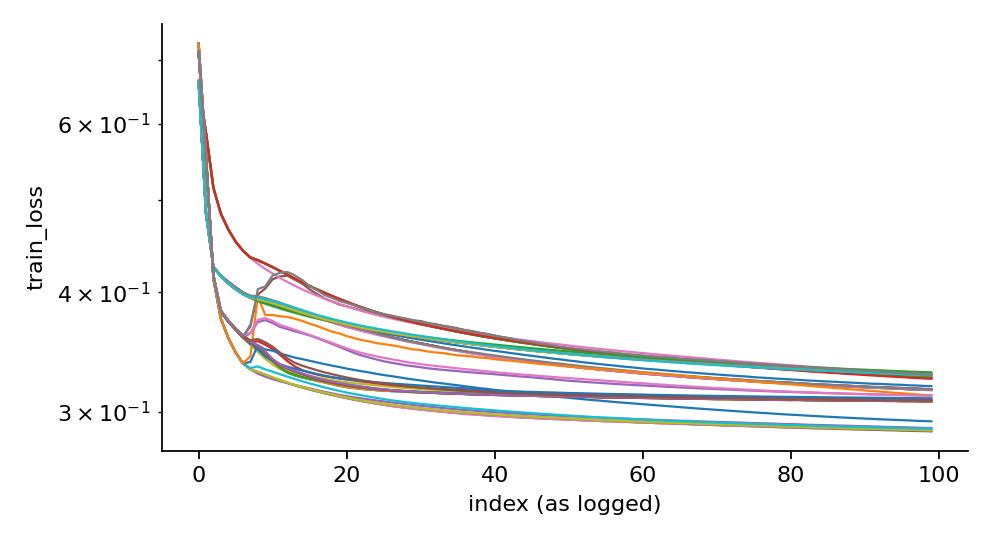
\includegraphics[width=\textwidth]{curve_train_loss.png}
\caption{\texttt{train\_loss}, the mean over seeds per cell.}
\label{fig:curve-1}
\end{figure}
\begin{figure}[tbp]
\centering
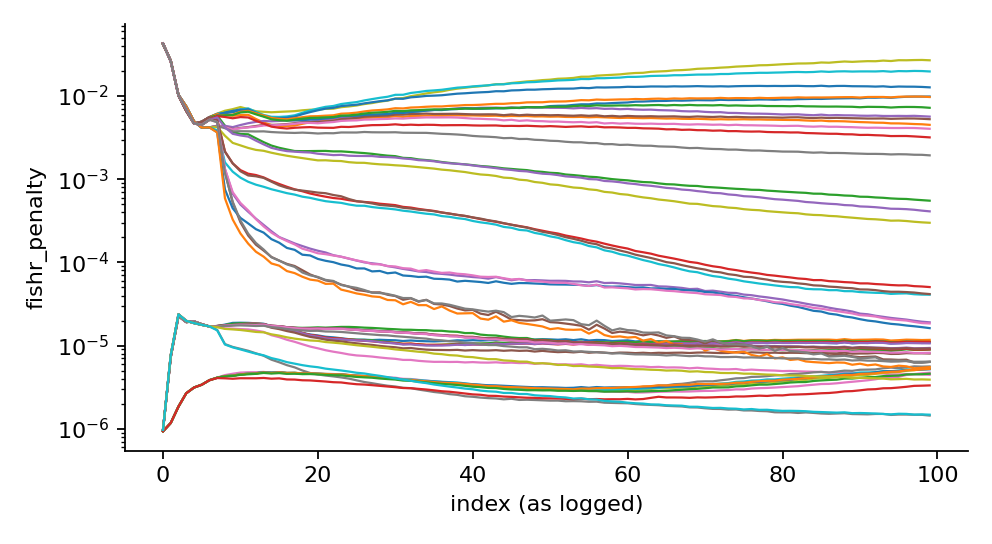
\includegraphics[width=\textwidth]{curve_fishr_penalty.png}
\caption{\texttt{fishr\_penalty}, the mean over seeds per cell.}
\label{fig:curve-2}
\end{figure}
\begin{figure}[tbp]
\centering
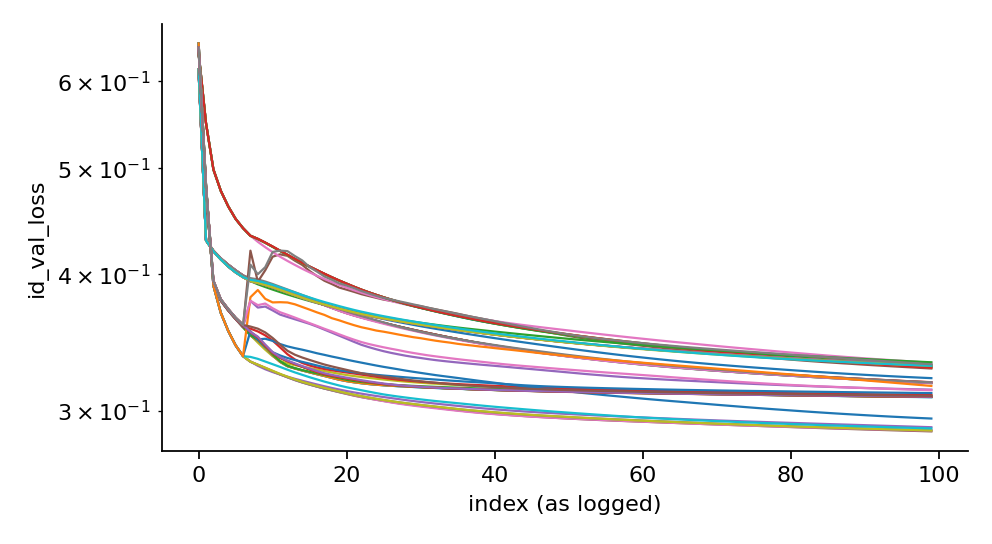
\includegraphics[width=\textwidth]{curve_id_val_loss.png}
\caption{\texttt{id\_val\_loss}, the mean over seeds per cell.}
\label{fig:curve-3}
\end{figure}

\section{Configuration}
The base configuration every run shares (frozen hash \texttt{057e46d824d4}); factor levels are in \autoref{tab:summary-ood_len_f1}.
{\footnotesize
\begin{verbatim}
task:
  name: KnapsackDataset
  value_range:
  - 1
  - 10
  target_range:
  - 10
  - 20
  weight_range:
  - 1
  - 10
  adversarial_range:
  - 10
  - 30
  noise_prob: 0.0
data:
  train_lengths:
  - 4
  - 5
  - 6
  - 7
  - 8
  ood_lengths:
  - 12
  - 16
  - 64
  ood_value_range:
  - 11
  - 21
  ood_noise_range:
  - 10
  - 30
  ood_noise_prob: 0.5
  n_per_length: 20000
  n_eval_per_length: 2000
  curve_eval_limit: 256
model:
  d_model: 64
  n_heads: 2
  num_layers: 1
  dropout: 0.0
  tropical_impl: legacy
optim:
  lr: 0.0001
  epochs: 100
  batch_size: 100
  eval_batch_size: 256
fishr:
  ema: 0.95
  anneal_iters: 1500
  reset_optimizer: true
\end{verbatim}
}
Store: \texttt{campaigns/tropical/Knapsack/results}.
\end{document}